% ******************************* PhD Thesis Template **************************
% Please have a look at the README.md file for info on how to use the template

% **************************** Formatting & Metadata ***************************

\documentclass[a4paper,12pt,times,print,custombib,chapter]{_Meta/thesis}
% See README.md for option details

\input{_Meta/preamble} %Contains packages and user-defined commands and settings
%
%% ************************ Thesis Information & Meta-data **********************
%
% ************************ Thesis Information & Meta-data **********************
%% The title of the thesis
\title{Characterising antibody immunity and ageing in a short-lived teleost}

%% Subtitle (Optional)
%\subtitle{}
%\submissiontext

%% The full name of the author
\author{William John Bradshaw}

%% Department (eg. Department of Engineering, Maths, Physics)
\dept{aus Hastings} %! Really?

%% University and Crest
%\university{University of Cologne, Germany}
% Crest minimum should be 30mm.
\crest{\includegraphics[width=0.5\textwidth]{_Meta/Logos/UoC_Crest}}

%% Use this crest, if you are using the college crest
%% Crest long miminum should be 65mm
%\crest{\includegraphics[width=0.45\textwidth]{University_Crest_Long}}

%% College shield [optional] 
% Crest minimum should be 30mm.
%\collegeshield{\includegraphics[width=0.2\textwidth]{CollegeShields/Kings}}


% Supervisor (optional)
% for multiple supervisors, append each supervisor with the \newline command
\supervisor{Dr. Dario Riccardo Valenzano\newline Prof. Dr. Andreas Beyer}

%% Supervisor line width: required to align supervisors
\supervisorlinewidth{\textwidth}


%% You can redefine the submission text:
% Default as per the University guidelines:
% ``This dissertation is submitted for the degree of''
%\renewcommand{\submissiontext}{change the default text here if needed}

%% Full title of the Degree
%\degreetitle{Doctor of Philosophy}

%% College affiliation (optional)
%\college{MPI for Biology of Ageing}

%% Submission date
% Default is set as {\monthname[\the\month]\space\the\year}
%\degreedate{September 2014} 

%%% Meta information
%\subject{LaTeX} \keywords{{LaTeX} {PhD Thesis} {Engineering} {University of
%Cambridge}}
 % Thesis title and author information, other metadata

% ***************************** Abstract Separate ******************************
% To printout only the titlepage and the abstract with the PhD title and the
% author name for submission to the Student Registry, use the `abstract' option in
% the document class.

\ifdefineAbstract
 \pagestyle{empty}
 \includeonly{A_Frontmatter/2_abstract-de,A_Frontmatter/3_abstract-en,C_Backmatter/declaration}
\fi

% ***************************** Chapter Mode ***********************************
% The chapter mode allows user to only print particular chapters with references
% Title, Contents, Frontmatter are disabled by default
% Useful option to review a particular chapter or to send it to supervisior.
% To use choose `chapter' option in the document class

\ifdefineChapter
	%\includeonly{B_Chapters/1_Introduction}
	%\includeonly{B_Chapters/2_Methods,C_Appendices/Solutions,C_Appendices/Primers,C_Appendices/Diversity,C_Appendices/Tables}
	%\includeonly{B_Chapters/3_Locus,C_Appendices/Figures,C_Appendices/Tables}
	\includeonly{B_Chapters/4_IgSeq,C_Appendices/Diversity,C_Appendices/Figures,C_Appendices/Tables}
	%\includeonly{C_Appendices/Solutions,C_Appendices/Primers,C_Appendices/Diversity,C_Appendices/Figures,C_Appendices/Tables}
\fi

\begin{document}
\maketitle

%% ******************************** Front Matter ********************************
%% Dedication, abstracts, acknowledgements etc. - do this last.

\frontmatter
% ******************************* Thesis Dedidcation ********************************

\begin{dedication} 
\doublespacing
\raggedleft
\textit{
\begin{LARGE}
Cre\'{e}r, c'est recombiner.\\
\end{LARGE}
-- Fran\c{c}ois Jacob \citep{hsu2015pathogen}}
\end{dedication}


% ************************** Thesis Abstract *****************************
% Use `abstract' as an option in the document class to print only the titlepage and the abstract.
\begin{zusammenfassung}
\end{zusammenfassung}
% ************************** Thesis Abstract *****************************
% Use `abstract' as an option in the document class to print only the titlepage and the abstract.
\begin{abstract}
\textbf{Motivation:} %Circular RNAs are a special class of RNA forming a covalently closed loop through a process called back-splicing. Not much is known about the function of circRNAs. Only for a few well studied circRNAs, potential functions were shown, these include miRNA sponging, RNA binding protein (RBP) sponging, and regulation of their host gene's transcription. Circular RNAs can be identified in rRNA depleted RNA-Sequencing by detecting chimeric reads, which span a back-splice junction. A variety of circRNA detection tools exists but no tool is able to summarize and characterize the identified circRNAs. To perform accurate downstream analyses after circRNA detection, it is crucial to know the exact exon-intron structure of circRNAs. Recently, two tools were published, which identify alternative splicing within circRNAs. Here, I am presenting \texttt{FUCHS} and \texttt{FUCHS\textit{denovo}} to summarize circRNAs and reconstruct their exon-intron chain based on liner-splice signals of back-splice junction anchored reads.

\textbf{Methods:} %In this study, I compared three state of the art circRNA detection programs. Based on the best tool, I developed a Python-based pipeline called \texttt{FUCHS}: \textbf{FU}ll \textbf{CH}aracterization of circular RNA using RNA-\textbf{S}equencing. This pipeline summarizes circRNAs by their host genes, detects skipped exons, finds double-breakpoint fragments, generates circle-wise coverage profiles, and clusters these profiles. Running \texttt{FUCHS} on a mouse dataset indicated that annotated gene models are not always suited to describe the circRNA's exon-intron structure. Hence, I developed an additional module, \texttt{FUCHS\textit{denovo}}, to reconstruct the exon-intron structure based on linear-splice signals of back-splice junction anchored reads. To demonstrate how \texttt{FUCHS} and \texttt{FUCHS\textit{denovo}} perform, I ran both programs on a dataset of young and old murine hearts and young and old murine livers.

\textbf{Results:} %The comparison of three circRNA detection programs (\texttt{DCC}, \texttt{CIRI}, and \texttt{KNIFE}) indicated \texttt{DCC} as the fastest and most accurate circRNA detection program. Running \texttt{FUCHS} on four mouse samples revealed that heart circRNAs are less diverse but more abundant than liver circRNAs. Considering only annotated exons, the average length of circRNAs was 500 BP. Heart circRNAs were longer than liver circRNAs. From the obtained coverage profiles, I concluded that annotated gene models were not always matching the exon-intron structure of circRNAs. A \textit{de novo} reconstruction of the inner circle structure using \texttt{FUCHS\textit{denovo}} showed a gain of information of 15 \%. Furthermore, \texttt{FUCHS\textit{denovo}} identified alternative splicing in 8 - 10 \% of circRNAs. Performing a differential motif enrichment analysis of the flanking introns of circRNAs with alternative splicing over circRNAs without alternative splicing identified FOXO as a potential transcription factor driving alternative splicing in circRNAs. Binding motifs for CPEB1 and HOX were enriched in the flanking introns of circRNAs from host genes expressing many circRNAs over circRNAs from host genes expressing only one circRNA. To exemplify the value of the reconstructed circRNA models in downstream analyses, I performed a miRNA seed search and RBP motif search. Comparing the seed density of circRNAs and mRNAs showed that circRNAs were more densely populated with both, miRNA seeds and RBP motifs. This suggests that circRNAs could form an additional layer in the gene-regulatory network by competing with their host genes for miRNA or RBP binding.

\textbf{Availability:} %\url{https://github.com/dieterich-lab/FUCHS.git}

\end{abstract}

% ************************** Thesis Acknowledgements **************************

\begin{acknowledgements}      

\dots

In the biomedical sciences at least, a doctoral thesis might have a single author but almost always has a great many contributors. Mine is no exception, and so I have a number of people to thank.

First, my thanks to Dr Dario Valenzano, who welcomed me into his research group ... % TODO: Finish this
and has always been an enthusiastic, attentive and understanding supervisor.

Many past and present members of the Valenzano group have actively contributed to the projects described in these pages. Dr Patrick Smith performed the microbiota-transfer studies that were the inspiration for the project in the first place and supervised and mentored me through my first and most difficult year. Dr Rongfeng Cui performed the genome assembly that was the foundation of the work in \Cref{chap:locus} and has provided a great deal of essential advice on both experimental procedures and computational analysis. David Willemsen has also been an essential provider of advice, insight and occasionally code, particularly for the more evolutionary parts of \Cref{chap:locus}. My student supervisees, Linda Zirden, Lena Schlautmann, Pascha Hokama, and especially Davina Patel all made essential contributions to developing and testing the turquoise-killifish immunoglobulin-sequencing protocol; you were all great. Our tireless and wonderful technician, Aleksandra Placzek, has been an essential part of the \igseq project in the lab and performed several of the library preps; several of my favourite parts of this thesis would not have been possible without her. Most recently, Michael Poeschla has joined the repertoire-sequencing team and helped prepare the libraries for the final \igseq experiment in \Cref{chap:igseq}, as well as providing many ... and exciting suggestions for future extensions of the work. I am sincerely grateful to all of them for their help in making my project what it is today. My thanks also to the rest of the Valenzano lab, particularly my fellow past and present students Jens Seidel, Miriam Popkes, Daniel Davila and Dr Franzi Metge, for making ...


% TODO: Collaborators

Kathrin Reichwald provided me with essential BAC clones and a substantial amount of important advice.  

Drs John Beausang, Aleksandra Walczak, Thierry Mora and Susana Magadan helped me get started with the enormous and intimidating world of immune repertoire analysis, and Aleksandra in particular has repeatedly provided invaluable advice, introductions and insight. Jason Vander Heiden has tirelessly answered my many questions about the Immcantation pipeline and even made some changes to it on my request, while Quentin Marcou has been an invaluable help in getting to grips with his wonderful software IGoR. Many other researchers have responded to my pestering emails, given advice where I needed it, and generally been friendly, welcome and generous with their time. I am grateful to you all.

The co-ordination team of the Cologne Graduate School of Ageing Research has consistently been amazing, and I have repeatedly been impressed at the depth of their dedication, sympathy and willingness to help us students with all our big and little problems. My sincerest thanks to Dr Daniela Morick, Dr Doris Birker and Jenny Ostermann for all your help and support.
% TODO: Ruth?

% TODO: Family

Finally, my deepest and sincerest thanks to Simon Woolf, without whom this entire long adventure would have been a great deal more difficult and a great deal less fun.

%Special thanks goes to my parents and my grandma for always believing in me, for their constant support and everything they taught me. Many thanks to Melanie M., Ariadna P., Brittany G., and Dennis S. for always listening to me and always having my back. My volleyball team for the right balance between work and exercise. My extended family, especially my family in Minnesota for their support and the possibilities they facilitated.\\
%Last but not least, I would like to thank everybody who helped me become who I am and where I am today. I am eternally grateful.

\end{acknowledgements}

\chapter{List of abbreviations}
\begin{abbreviations}
\item[A3SS] Alternative 3' spice site
\item[A5SS] Alternative 5' spice site
\item[AEU] Alternative exon usage
\item[AGO-PARCLIP] Argonaute PAR-CLIP
\item[AS] Alternative splicing
\item[BP] Base pair
\item[BSJ] Back-splice junction
%\item[CDR1] cerebellar degeneration-related protein 1
\item[circExon] Circularized exon
\item[circRNA] Circular RNA
\item[CNS] Central nervous system
\item[DNA] Deoxyribonucleic acid
\item[EMT] Epithelial mesenchymal transition
\item[ES] Exon skipping
\item[FDR] False discovery rate
\item[FP] False positive
\item[GFP] Green fluorescent protein
\item[GO] Gene ontology
\item[IR] Intron retention
\item[lncRNA] Long non-coding RNA
%\item[MBNL1] muscleblind
\item[miRNA] Micro RNA
\item[mRNA] Messenger RNA
\item[PAR-CLIP] Photoactivatable-ribonucleoside-enhanced crosslinking and immunoprecipitation
\item[PCR] Polymerase chain reaction
%\item[PolII] Polymerase II
%\item[QKI] Quaking
\item[qPCR] Quantitative PCR
\item[RCM] Reverse complementary matches
\item[RNA] Ribonucleic acid
\item[RNA-Seq] RNA-Sequencing
\item[rRNA] Ribosomal RNA
\item[siRNA] Small interfering RNA
\item[snoRNA] Small nucleolar RNA
\item[SNP] Small nucleotide polymorphism
\item[TER] Transcription elongation rate
\item[TF] Transcription factor
\item[TP] True positive
\item[tRNA] Transfer RNA
\item[TSS] Transcription start site

\end{abbreviations}

%% *********************** Adding TOC and List of Figures ***********************
%%%
\tableofcontents
%%
\listoffigures
%%
\listoftables
%%
\setlength{\glslistdottedwidth}{4cm}
\setglossarystyle{listdotted}
\printglossary[title={List of abbreviations},nonumberlist=true,nogroupskip=true]

%
%\chapter{List of abbreviations}
\begin{abbreviations}
\item[A3SS] Alternative 3' spice site
\item[A5SS] Alternative 5' spice site
\item[AEU] Alternative exon usage
\item[AGO-PARCLIP] Argonaute PAR-CLIP
\item[AS] Alternative splicing
\item[BP] Base pair
\item[BSJ] Back-splice junction
%\item[CDR1] cerebellar degeneration-related protein 1
\item[circExon] Circularized exon
\item[circRNA] Circular RNA
\item[CNS] Central nervous system
\item[DNA] Deoxyribonucleic acid
\item[EMT] Epithelial mesenchymal transition
\item[ES] Exon skipping
\item[FDR] False discovery rate
\item[FP] False positive
\item[GFP] Green fluorescent protein
\item[GO] Gene ontology
\item[IR] Intron retention
\item[lncRNA] Long non-coding RNA
%\item[MBNL1] muscleblind
\item[miRNA] Micro RNA
\item[mRNA] Messenger RNA
\item[PAR-CLIP] Photoactivatable-ribonucleoside-enhanced crosslinking and immunoprecipitation
\item[PCR] Polymerase chain reaction
%\item[PolII] Polymerase II
%\item[QKI] Quaking
\item[qPCR] Quantitative PCR
\item[RCM] Reverse complementary matches
\item[RNA] Ribonucleic acid
\item[RNA-Seq] RNA-Sequencing
\item[rRNA] Ribosomal RNA
\item[siRNA] Small interfering RNA
\item[snoRNA] Small nucleolar RNA
\item[SNP] Small nucleotide polymorphism
\item[TER] Transcription elongation rate
\item[TF] Transcription factor
\item[TP] True positive
\item[tRNA] Transfer RNA
\item[TSS] Transcription start site

\end{abbreviations}
%\printnomenclature[space] space can be set as 2em between symbol and description
%\printnomenclature[3em]

%\printnomenclature
%
%% ******************************** Main Matter *********************************
\mainmatter\onehalfspacing
%
\include{B_Chapters/1_Introduction}
\chapter{Materials and methods}  
\onehalfspacing

\ifdefineChapter
	{\LARGE Second Draft, \today}
\fi

\pagebreak

\section{Killifish husbandry and sample preparation methods}
\label{sec:methods_husbandry}

Male turquoise killifish (\nfu, GRZ-AD strain) from a single hatching were raised under standard husbandry conditions \parencite{dodzian2018husbandry} and housed from four weeks post-hatching in individual \lt{2.8} tanks connected to a water recirculation system. Fish received \hr{12} of light per day on a regular light/dark cycle, and were fed blood
worm larvae and brine shrimp nauplii twice a day during the week and once a day during the weekend \parencite{dodzian2018husbandry,smith2017microbiota}.

Sacrificed fish (\Cref{tab:igseq-cohorts-fish}) were killed by anaesthetisation in \gl{1.5} Tricaine solution in room-temperature tank water \parencite{carter2011tricaine}, then flash-frozen in liquid nitrogen and ground to a homogenous powder with a pestle in a liquid-nitrogen-filled mortar. The powder was mixed thoroughly and stored at \degC{-80} prior to RNA isolation.

\section{Biochemistry and molecular biology methods}

\subsection{Standard methods}

\subsubsection{PCR}
\label{sec:methods_molec_standard_pcr}

The polymerase chain reaction is a well-established method for rapid amplification of a DNA sequence through repeated cycles of denaturation, primer-annealing and replication by a high-temperature-tolerant DNA polymerase enzyme \parencite{paul2010hotstartpcr}. Unless otherwise specified, all PCRs in this chapter were performed using \x{2} Kapa HiFi HotStart ReadyMix PCR Kit (\Cref{app:solutions_enzymes}) according to the manufacturer's instructions. Briefly, for a \ul{25} reaction, \ul{12.5} Kapa ReadyMix was combined with \ul{12.5} total of template, nuclease-free water, and primers; these volumes were scaled linearly for reactions of different volumes. The mixture was then heated in a thermocycler as described in \Cref{tab:kapa}.

\begin{table}[h]
\centering
\caption{Thermocycler protocol for Kapa high-fidelity hot-start PCR}
\label{tab:kapa}
\begin{threeparttable}
\begin{tabular}{cccc}\toprule
\textbf{Step} & \textbf{Temperature [\degC{}]} & \textbf{Duration [\secs{}]} & \textbf{Cycles}\\\midrule
Initial denaturation & 95 & 180 & 1 \\\midrule
Denaturation & 98 & 20 & \multirow{3}{*}{$n_c$\tnote{a}}\\
Annealing & $T_a$\tnote{a} \tnote{} & 15 & \\
Extension & 72 & $t_{ext}$\tnote{a} & \\\midrule
Final extension & 72 & $t_{ext} \times 4$\tnote{a} & 1\\
\bottomrule\end{tabular}
\begin{tablenotes}
\item[a] Annealing temperature ($T_a$), extension time ($t_{ext}$) and cycle number ($n_c$) determined separately for each reaction.
\end{tablenotes}
\end{threeparttable}
\end{table}

\subsubsection{Nucleic-acid purification with SeraSure magnetic beads}
\label{sec:methods_molec_standard_serasure}

Nucleic-acid isolation, size-selection and concentration in the \igseq library-preparation protocol (and elsewhere where necessary) were performed using SeraSure SPRI (solid phase reversible immobilization) bead preparations \parencite{hawkins1994spri,deangelis1995spri,lennon2010cleanup,fisher2011cleanup}. In SPRI, carboxyl-coated paramagnetic beads bind DNA in the presence of polyethylene glycol (PEG), with the affinity of the beads for DNA depending on the concentration of PEG in the binding buffer. As a result, the range of nucleic-acid sequence lengths retained by SPRI bead purification depends primarily on the concentration of PEG, which in turn depends on the relative volume of SeraSure bead suspension added to a sample; the higher the concentration, the shorter the minimum fragment length retained during the purification process. In combination with a magnetic rack to remove the DNA-bound beads from suspension, this allows DNA of the desired size range to be isolated from a solution and resuspended in the desired volume of fresh buffer.

To prepare \ml{50} of SeraSure bead suspension for DNA (or DNA:RNA heteroduplex) isolation, a stock of SeraMag beads (\Cref{app:solutions_reagents}) was vortexed thoroughly, and \ml{1} was transferred to a new tube. This tube was then transferred to a magnetic rack and incubated at room temperature for \mins{1}, then the supernatant was removed and replaced with \ml{1} TET buffer (\Cref{app:solutions_buffers}) and the tube was removed from the rack and vortexed thoroughly. This washing process was repeated twice more, for a total of three washes in TET. A fourth cycle was used to replace the TET with incomplete SeraBind buffer (iSB, \Cref{app:solutions_buffers}). The vortexed \ml{1} aliquot of beads in iSB was then transferred to a conical tube containing \ml{28} iSB and mixed by inversion. To add the PEG, \ml{20} \pc{50} (w/v) PEG 8000 solution was dispensed slowly down the side of the conical tube, bringing the total volume to \ml{49}. Finally, this was brought to \ml{50} by adding \ul{250} \pc{10} (w/v) Tween 20 solution and \ul{750} autoclaved water to complete the SeraSure bead suspension.

To perform a bead cleanup, an aliquot of prepared SeraSure suspension was vortexed thoroughly to completely resuspend the beads, then the appropriate relative volume of SeraSure suspension was added to a sample, mixing thoroughly by gentle pipetting. The sample was incubated at room temperature for \mins{5} to allow the beads to bind the DNA, then transferred to a magnetic rack and incubated for a further \mins{5} to draw as many beads as possible out of suspension. The supernatant was removed and discarded and replaced with \pc{80} ethanol, to a volume sufficient to completely submerge the bead pellet. The sample was incubated for 0.5-\mins{1}, then the ethanol was replaced and incubated for a further 0.5-\mins{1}. The second ethanol wash was removed, and the tube left on the rack until the bead pellet was almost, but not completely, dry, after which it was removed from the rack. The bead pellet was resuspended in a suitable volume of elution buffer (EB, \Cref{app:solutions_buffers}) then incubated at room temperature for at least 5 minutes to allow the nucleic-acid molecules to elute from the beads.

Unless otherwise specified, the beads from a cleanup were left in a sample during subsequent applications. To remove beads from a sample, the sample was mixed gently but thoroughly to resuspend the beads, incubated for an extended time period (at least \mins{10}) to maximise nucleic-acid elution, then transferred to a magnetic rack and incubated for 2-\mins{5} to remove the beads from suspension. The supernatant (containing the eluted nucleic-acid molecules) was then transferred to a new tube, and the beads discarded.

\subsubsection{Phenol-chloroform extraction and ethanol precipitation of DNA}
\label{sec:methods_molec_standard_phenol}

Phenol-chloroform extraction is a well-established method for removing proteins and other hydrophobic or amphipathic contaminants from nucleic-acid solutions \parencite{zumbo2012phenolchloroform}. By thoroughly mixing an aqueous solution of nucleic acid with an organic solvent (phenol), hydrophobic contaminants are dissolved into the organic phase while proteins are denatured at the organic/aqueous boundary. The addition of chloroform further encourages the denaturation of proteins, as well as improving separation of the aqueous and organic phases following centrifugation. The effect on nucleic acids depends upon the pH of the phenol: under acidic conditions, the negatively-charged DNA phosphate backbone is neutralised and so primarily dissolves in the organic phase, while RNA is kept in the aqueous phase through hydrogen bonding between water and exposed bases; under neutral or basic conditions, both DNA and RNA are retained in the aqueous phase \parencite{zumbo2012phenolchloroform}.

To remove protein from isolated DNA samples, each sample was diluted to \ul{500} in nuclease-free water and mixed with \ul{500} of equilibrated (non-acidic) phenol:chloroform:isoamyl alcohol (PCI) mixture (\Cref{app:solutions_reagents}) in a fume hood. The sample/PCI mixture was shaken vigorously by hand for \secs{15} to thoroughly mix the different components, then centrifuged in a benchtop centrifuge (\mins{5}, room temperature, top speed). Again in a fume hood, the mixed sample was held at an angle, and the upper aqueous phase containing the DNA was removed and transferred to a new tube while the lower organic phase was discarded. A second aliquot of \ul{500} PCI was added and the sample was mixed, centrifuged and separated as before. Finally, in order to remove residual phenol in the sample, \ul{500} pure chloroform was added to the newly-separated aqueous phase and the sample was once again mixed, centrifuged and separated. 

Following this final round of separation, the DNA in the aqueous phase was re-isolated using ethanol precipitation, another widely-used protocol exploiting the ability of alcohols to precipitate nucleic acids in the presence of monovalant cations \parencite{zumbo2012ethanol}. 0.1 volumes of \mol{3} sodium acetate solution was added to each sample, followed by 2.5 volumes of fresh \pc{100} ethanol. The mixture was mixed gently by inversion, then incubated for 1-\hr{3} at \degC{-80} or at \degC{-20} overnight. The suspension of precipitated DNA was pelleted through centrifugation in a benchtop centrifuge (\mins{30}, \degC{4}, top speed). The supernatant was discarded and replaced with \ul{500} chilled \pc{70} ethanol, and the sample centrifuged again (\mins{5}, \degC{4}, top speed). After this, the supernatant was again discarded, and the samples allowed to air-dry before being resuspended in 30-\ul{50} EB (\Cref{app:solutions_buffers}). 

\subsubsection{Guanidinium thiocyanate-phenol-chloroform extraction of RNA}
\label{sec:methods_molec_standard_qiazol}

Guanidinium thiocyanate-phenol-chloroform extraction is a technique for purifying RNA samples closely related to the phenol-chloroform-extraction method described in \Cref{sec:methods_molec_standard_phenol} \parencite{zumbo2012phenolchloroform}. By using acid rather than equilibrated phenol, DNA in the sample is dissolved in the organic rather than the aqueous phase and so is removed from the aqueous solution along with proteins and other contaminants \parencite{zumbo2012phenolchloroform,chomczynski2006trizol}. Meanwhile, the addition of guanidinium thiocyanate, a chaotropic agent which disrupts hydrogen bonds in aqueous solution, strongly encourages the rapid denaturation of proteins and so helps protect the RNA from degradation by RNase enzymes \parencite{zumbo2012phenolchloroform,chomczynski2006trizol}.

To isolate total RNA from homogenised killifish tissues, \ml{1} of QIAzol lysis reagent (\Cref{app:solutions_reagents}, containing acid phenol and guanidinium thiocyanate) was added to \gr{0.1} of tissue, mixed gently but thoroughly by inversion, then incubated at room temperature for \mins{5} to allow the QIAzol to penetrate the tissue. 0.2 volumes of chloroform was added and the mixture was shaken vigorously for \secs{15}, then incubated at room temperature for \mins{3}. The mixture was then centrifuged (\mins{15}, \degC{4}, \g{12000}). Holding the tube at an angle, the upper aqueous phase containing the RNA was removed and transferred to a new tube, while the lower organic phase was discarded.

Following phase separation, the RNA was precipitated using isopropanol precipitation, which works on the same principles as ethanol precipitation (\Cref{sec:methods_molec_standard_phenol}) but requires lower relative volumes of alcohol \parencite{zumbo2012ethanol}. 0.5 volumes of room-temperature isopropanol was added to each sample, mixing gently by inversion and incubating for \mins{5} at room temperature. The suspension was centrifuged (\mins{10}, \degC{4}, \g{12000}) and the supernatant discarded. 1 volume of freshly prepared \pc{75} ethanol was added and the tube was vortexed briefly and centrifuged again (\mins{5}, \degC{4}, \g{7500}). The supernatant was discarded and the RNA pellet allowed to air-dry for 5-\mins{10}, then resuspended in \ul{50} EB (\Cref{app:solutions_buffers}). The concentration and quality of the resulting total-RNA solution were assayed with the Qubit 2.0 flourometer (Thermo Fisher, RNA BR assay kit) and TapeStation 4200 (Agilent, RNA tape), respectively, according to the manufacturer's instructions.

\subsection{Library size-selection with the BluePippin}
\label{sec:methods_molec_standard_bluepippin}

The BluePippin (Sage Science) is a DNA size-selection system based on agarose gel electrophoresis, which uses timed switching between positively-charged electrodes at a forked gel channel in an agarose cassette to redirect DNA of a desired size range into a separate lane from the rest of the sample \parencite{sage2016bluepippin}. The timing of the switch is determined based on the size range input by the user and calibrated using flourescent internal standards, which are added to the sample during the sample preparation process and designed to run well ahead of the possible size ranges for that cassette type. The combination of the choice of cassette and the choice of standards determines which fragment lengths can be effectively isolated using the machine.

For the experiments described in this thesis, a \pc{1.5} cassette with R2 markers was used, enabling size selection of targets in the range of 250--\bp{1500} \parencite{sage2016bluepippin}. Machine calibration and testing, cassette preparation, and protocol design were performed in accordance with the BluePippin documentation and instructions given by the machine software. During this process, the elution wells of the lanes to be used in the size-selection run were emptied and refilled with \ul{40} of electrophoresis buffer (\Cref{app:solutions_reagents}), then sealed for the duration of the run, and a broad-range size-selection protocol with a target range of 400 to \bp{800} was specified. \ul{30} of sample was then combined with \ul{10} of loading solution (\Cref{app:solutions_reagents}) and vortexed to mix, then \ul{40} of buffer was removed from the appropriate loading well and replaced, slowly, with the prepared sample mixture. The protocol was started and run until the final elution was complete. Finally, the eluted samples were removed from the elution wells of the appropriate lanes, and the unused lanes of the cassette were re-sealed for future use.

\subsection{Isolation and sequencing of bacterial artificial chromosomes}
\label{sec:methods_molec_bacs}

All BAC clones that were sequenced for this research were provided by the FLI in Jena as plate or stab cultures of transformed \textit{E. coli}, which were replated and stored at \degC{4}. Prior to isolation, the clones of interest were cultured overnight in at least \ml{100} LB medium. The resulting liquid cultures were transferred to \ml{50} conical tubes and centrifuged (10-\mins{25}, \degC{4}, \g{3500}) to pellet the cells. The supernatant was carefully discarded and the cells were resuspended in \ml{18} buffer P1 (\Cref{app:solutions_buffers}).

After resuspension, the cultures underwent alkaline lysis \parencite{birnboim1979alkalinelysis} to release the BAC DNA and precipitate genomic DNA and cellular debris. \ml{18} buffer P2 (\Cref{app:solutions_buffers}) was added to each tube, which was then mixed gently but thoroughly by inversion and incubated at room temperature for \mins{5}. \ml{10} ice-chilled neutralisation buffer P3 (\Cref{app:solutions_buffers}) was added to precipitate genomic DNA and cellular debris, and each tube was mixed gently but thoroughly by inversion and incubated on ice for \mins{15}. The tubes were then centrifuged (20-\mins{30}, \degC{4}, \g{12000}) to pellet cellular debris and the supernatant was transferred to new conical tubes. This process was repeated at least two more times, until no more debris was visible in any tube; this repeated pelleting was necessary to minimise contamination in each sample, as the normal column- or paper-based filtering steps used during alkaline lysis resulted in the loss of the BAC DNA.

Following alkaline lysis, the DNA in each sample underwent isopropanol precipitation: 0.6 volumes of room-temperature isopropanol were added to the clean supernatant in each tube, followed by 0.1 volumes of \mol{3} sodium acetate solution. Each tube was mixed well by inversion, incubated for 10-\mins{15} at room temperature, then centrifuged (\mins{30}, \degC{4}, \g{12000}) to pellet the DNA. The supernatant was discarded and the resulting DNA smear was ``resuspended'' in \ml{1} \pc{100} ethanol and transferred to a \ml{1.5} tube, which was re-centrifuged (\mins{5}, \degC{4}, top speed) to obtain a concentrated pellet. Finally, the pelleted samples were resuspended in EB (\Cref{app:solutions_buffers}) and purified of proteins and RNA using phenol-chloroform extraction and ethanol precipitation (\Cref{sec:methods_molec_standard_phenol}).

The resuspended BAC isolates were sent to the Cologne Center for Genomics, where they underwent Illumina Nextera XT library preparation and were sequenced on an Illumina MiSeq sequencing machine (MiSeq Reagent Kit v3, 2x300bp reads).

\subsection{Immunoglobulin sequencing of killifish samples}
\label{sec:methods_molec_igseq}

\subsubsection{RNA template quantification and quality control}
\label{sec:methods_molec_igseq_template}

Total RNA from whole-body killifish samples was isolated as described in \Cref{sec:methods_molec_standard_qiazol}; gut RNA from microbiota transfer experiments \parencite{smith2017microbiota} was already prepared and available. Quantification of RNA samples was performed with the Qubit 2.0 flourometer (Thermo Fisher, RNA BR assay kit), while quality control and integrity measurement was performed using the TapeStation 4200 (Agilent, RNA tape), both according to the manufacturer's instructions.

\subsubsection{Reverse-transcription and template switching}
\label{sec:methods_molec_igseq_rt}

Reverse transcription of total RNA and template switching for \igseq library preparation was performed using SMARTScribe Reverse Transcriptase (\Cref{app:solutions_enzymes}), in line with the protocol specified in Turchaninova \textit{et al.} \parencite{turchaninova2016igprep}. Briefly, \ng{750} total RNA from a killifish sample was combined with \ul{2} \umol{10} gene-specific primer (GSP), homologous with the second \ch exon of \Nfu \igh{M} (\Cref{app:oligos_primers}, designed using \program{Primer3} \parencite{untergasser2012primer3}). The reaction volume was brought to a total of \ul{8} with nuclease-free water, and the resulting mixture was incubated for 2 minutes at \degC{70} to denature the RNA, then cooled to \degC{42} to anneal the GSP \parencite{turchaninova2016igprep}.

Following annealing, the RNA-primer mixture was combined with \ul{12} of reverse-transcription master-mix (\Cref{tab:methods_rt_mm}), including the reverse-transcriptase enzyme and template-switch adapter (\Cref{app:oligos_tsa}, sequence provided in \parencite{turchaninova2016igprep}). The complete reaction mixture was incubated for \hr{1} at \degC{42} for the reverse-transcription reaction, then mixed with \ul{1} of uracil DNA glycosylase (UDG, \Cref{app:solutions_enzymes}) and incubated for a further \mins{40} at \degC{37} to digest the template-switch adapter. Finally, the reaction product was purified using SeraSure beads (\Cref{sec:methods_molec_standard_serasure}) at \x{0.7} concentration, eluting in \ul{16.5} clean elution buffer (EB, \Cref{app:solutions_buffers}).

\begin{table}[h]
\begin{center}\small
\begin{threeparttable}
\caption[Master-mix components for SMARTScribe reverse transcription]{Master-mix components for SMARTScribe reverse transcription (per sample)}
\begin{tabular}{llll}\toprule
\textbf{Volume [\ul{}]} & \textbf{Component} & \textbf{Concentration} & \textbf{Reference}\\\midrule
2 & SMARTScribe reverse transcriptase & \unitsul{100} & \Cref{app:solutions_enzymes} \\
4 & SMARTScribe first-strand buffer & \x{5} & \Cref{app:solutions_reagents} \\
2 & SmartNNNa barcoded TSA & \umol{10} & \Cref{app:oligos_tsa}\\
2 & DTT & \mmol{20} & \Cref{app:solutions_reagents}\\
2 & dNTP mix & \umol{10} per nucleotide & \Cref{app:solutions_reagents}\\
0.5 & RNasin RNase inhibitor & \unitsul{40} & \Cref{app:solutions_enzymes}\\\bottomrule
\end{tabular}
\label{tab:methods_rt_mm}
\end{threeparttable}
\end{center}
\end{table}

\subsubsection{PCR amplification and adapter addition} 
\label{sec:methods_molec_igseq_pcr}

Following reverse-transcription, UDG digestion, and cleanup, the reaction mixture underwent three successive rounds of Kapa PCR (\Cref{sec:methods_molec_standard_pcr}, \Cref{tab:methods_igseq_pcr}) each of which was followed by a further round of bead cleanups (\Cref{sec:methods_molec_standard_serasure}, \Cref{tab:methods_igseq_beads}). The first of these PCR reactions added a second strand to the reverse-transcribed cDNA and amplified the resulting DNA molecules; the second added partial Illumina sequencing adapters and further amplified the library, and the third added complete Illumina adapters (\Cref{app:oligos_illumina}, including i5 and i7 indices \parencite{illumina2018adapters}). Primer sequences (\Cref{app:oligos_primers}) homologous to the template-switch adapter (M1SS and M1S) were provided by \parencite{turchaninova2016igprep}, while those homologous to the \cm{1} constant-region exon (IGHC-B and IGHC-C) were designed using \program{Primer3} \parencite{untergasser2012primer3}; as with the GSP in \Cref{sec:methods_molec_igseq_rt}, all PCR primers were diluted to and stored at \umol{10} prior to use.

\begin{table}[h]
\def\arraystretch{1.3}
\centering\small
\begin{threeparttable}
\caption{PCR protocols for \Nfu immunoglobulin sequencing}
\begin{tabular}{c|ccc|cc|ccccc}\toprule
\multirow{2}{*}{\textbf{PCR}} & \multicolumn{3}{c|}{\textbf{Protocol details}} & \multicolumn{2}{c|}{\textbf{Primers}} & \multicolumn{4}{c}{\textbf{Volumes (\ul{})\tnote{b}}}\\
 & \# cycles & $T_m$ (\degC{}) & $t_\mathrm{ext}$ (\secs{}) & F & R & Template & Primers\tnote{c} & Kapa & H\textsubscript{2}O \\\midrule
1 & 18 & 65 & 15 & IGHC-B & M1SS & 10.5 & 1 (\x{}2) & 12.5 & 0 \\\midrule
2 & 13 & 65 & 15 & M1S+P2 & IGHC-C+P1 & 1 & 0.5 (\x{}2) & 12.5 & 10.5 \\\midrule
3 & 7 to 12\tnote{d} & 68 & 15 & D50*\tnote{a} & D7**\tnote{a} & 2 & 0.75 (\x{}2) & 12.5 & 9 \\
\bottomrule
\end{tabular}
\begin{tablenotes}
\item[a] PCR3 primers selected as appropriate for each library's assigned indices; see \Cref{app:oligos_illumina} for more information.
\item[b] If the number of samples to be sequenced was small, all volumes of PCR 3 were doubled for a \ul{50} total PCR volume.
\item[c] Stated volume applies separately to both forward and reverse primer for that reaction. Primers were diluted to and stored at \umol{10} prior to use.
\item[d] See \Cref{tab:methods_igseq_cycles} for specific cycle numbers used in each experiment.
\end{tablenotes}
\label{tab:methods_igseq_pcr}
\end{threeparttable}
\end{table}

\begin{table}[h]
\def\arraystretch{1.5}
\centering\small
\caption{Bead cleanups during \Nfu immunoglobulin sequencing}
\begin{threeparttable}
\begin{tabular}{l|c|cc|c}\toprule
\multirow{2}{*}{\textbf{Stage}\tnote{a}} & \multirow{2}{*}{\textbf{Sample volume}} & \multicolumn{2}{c|}{\textbf{Beads volume (\ul{})}} & \multirow{2}{*}{\textbf{Elution volume (\ul{})}\tnote{c}}\\
& & \ul{} & \x{}\tnote{b} & \\\midrule
RT & 21 & 14.7 & 0.7 & 16.5\\
PCR 1 & 25 & 17.5 & 0.7 & 25\\
PCR 2 & 25 & 17.5 & 0.7 & 15\\
PCR 3 & 25\tnote{d} & 20\tnote{d} & 0.8 & 15\tnote{d}\\
Pooling & Varies\tnote{e} & Varies\tnote{e} & 2.5 & 35\\ 
\bottomrule
\end{tabular}
\begin{tablenotes}
\item[a] Each bead cleanup takes place immediately \textit{after} its corresponding stage.
\item[b] Bead volumes are usually given as multiples of the sample volume.
\item[c] All elutions performed in the specified volume of elution buffer (EB, \Cref{app:solutions_buffers}).
\item[d] If PCR 3 reaction volume differs from \ul{25}, bead and elution volumes are rescaled proportionally to sample volume as appropriate.
\item[e] Samples are pooled in equimolar ratio.
\end{tablenotes}
\label{tab:methods_igseq_beads}
\end{threeparttable}
\end{table}

\begin{table}[h]
\def\arraystretch{1.3}
\centering\small
\caption{PCR cycle numbers used for \Nfu immunoglobulin sequencing}
\begin{threeparttable}
\begin{tabular}{c|ccc|cc|ccccc}\toprule
\multirow{2}{*}{\textbf{Experiment}} & \multicolumn{3}{c|}{\textbf{Number of PCR cycles}} & \multirow{2}{*}{\textbf{Reference}}\\
& PCR 1 & PCR 2 & PCR 3 &\\\midrule
Pilot & 18 & 13 & 9 & \Cref{sec:igseq_pilot}\\
Ageing & 18 & 13 & 8 & \Cref{sec:igseq_ageing}\\
Gut & 18 & 13 & 12 &\Cref{sec:igseq_gut}\\
\bottomrule
\end{tabular}
\label{tab:methods_igseq_cycles}
\end{threeparttable}
\end{table}

\subsubsection{Library pooling, size selection and sequencing} 
\label{sec:methods_molec_igseq_seq}

Following PCR3 and its attendant bead cleanup, the total concentration of each library was assayed with the Qubit 2.0 (Thermo Fisher, DNA HS assay kit), while the size distribution of each library was obtained using the TapeStation 4200 (Agilent, D1000 tape). To obtain the concentration of complete library molecules in each case (as opposed to primer dimers or other off-target bands), the ratio between the concentration of the desired library band (c. 620-\bp{680}) and the total concentration of the sample was calculated for each TapeStation lane, and the total concentration of each library as measured by the Qubit was multiplied by this ratio to obtain an estimate of the desired figure:

\begin{equation}
\mathrm{Library~concentration}~(L) = \mathrm{Qubit~concentration} \times \frac{\mathrm{TapeStation~concentration~[main~band]}}{\mathrm{TapeStation~concentration~[total]}}
\label{eq:library-conc}
\end{equation}

\noindent All the libraries for a given experiment were then pooled, such that the estimated concentration $L$ of each library in the final pooled sample was equal and the total mass of nucleic acid in the pooled sample was at least \ng{240}. The pooled libraries underwent a final bead cleanup (\Cref{sec:methods_molec_standard_serasure}, \Cref{tab:methods_igseq_beads}) to concentrate the samples, then underwent size selection with the BluePippin (\Cref{sec:methods_molec_standard_bluepippin}, \pc{1.5} DF Marker R2, broad 400-800bp). The size-selected pooled samples underwent a final round of quality control with the Qubit and TapeStation (as above) to confirm their collective concentration (at least \nmol{1.5}) and size distribution (one peak at c. 620-\bp{680}). Finally, the pooled and size-selected libraries were sequenced on an Illumina MiSeq System (MiSeq Reagent Kit v3, 2x300bp reads, 30\,\% PhiX spike-in), either at the Cologne Center for Genomics (pilot and ageing experiments) or with Admera Health (gut experiment).

\section{Computational and analytic methods}
\label{sec:methods_comp}

Version details for software used in this section are given in \Cref{tab:software-versions}.

\subsection{General data processing, pipeline structure and data visualisation}
\label{sec:methods_comp_general}

Unless otherwise specified, processing and analysis of biological data was performed using standard Bioconductor \parencite{huber2015bioconductor} packages: \program{Biostrings} \parencite{pages2017biostrings} and \program{BSgenome} \parencite{pages2018bsgenome} for biological sequence data, \program{GenomicRanges} \parencite{lawrence2013genomicranges} for sequence ranges, and \program{genbankr} \parencite{becker2018genbankr} and \program{rentrez} \parencite{winter2017rentrez} for GenBank files. 

Smith-Waterman and Needleman-Wunsch exhaustive alignments \parencite{needleman1970alignment,waterman1981alignment} were performed using the \snippet{pairwiseAlignment} function from \program{Biostrings}; percentage sequence identities were computed using the \snippet{pid} function from the same package.

Processing of tabular data was performed using the Tidyverse suite of tools, especially \program{readr} \parencite{wickham2018readr}, \program{dplyr} \parencite{wickham2018dplyr}, \program{tidyr} \parencite{wickham2018tidyr} and \program{stringr} \parencite{wickham2018stringr}. \program{Snakemake} \parencite{koster2012snakemake} was used to design and run data-processing pipelines.

Unless otherwise specified, standard statistical operations and comparisons were performed using built-in functions from the \program{stats} package in \program{R} \parencite{rcore2018rcore}: \snippet{wilcox.test} for two-sample Mann-Whitney $U$ tests, \snippet{kruskal.test} for multisample Kruskal-Wallis analysis-of-variance tests, \snippet{lm} for linear models, \snippet{glm} for generalised linear models, \snippet{cor} for Pearson product-moment correlation coefficients, \snippet{hclust} for hierarchical clustering, and \snippet{pcoa} for principal co-ordinate analysis.

Unless otherwise specified, data were visualised using \program{ggplot2} \parencite{wickham2016ggplot2}. Chromosome ideograms, locus structure visualisations, and Sashimi plots \parencite{katz2013sashimi} were constructed using \program{Gviz} \parencite{hahne2016gviz}. Cluster dendrograms and phylogenetic trees were drawn with \program{ggtree} \parencite{guangchuang2018ggtree}, using utilities from \program{ape} \parencite{paradis2018ape} and \program{tidytree} \parencite{guangchuang2018tidytree}. Sequence logos were drawn with \program{ggseqlogo} \parencite{wagih2017ggseqlogo}. 

\subsection{BAC insert assembly}
\label{sec:methods_comp_bacs}

\subsubsection{Identifying BAC candidates for the \nfu \igh{} locus}
\label{sec:methods_comp_bacs_ident}

The first group of candidate BAC clones \parencite{reichwald2015genome} to be used in the \Nfu locus assembly was identified by searching for scaffolds in a previous assembly of the \Nfu genome (\texttt{NotFur1}, GenBank accession GCA\_000878545.1 \parencite{valenzano2015genome}) that contained either \textit{IGH} gene fragments (GapFilledScaffold\_8761, 8571, 16121) or genes homologous to those flanking the \textit{IGH} locus in stickleback and medaka (GapFilledScaffold\_2443 and 292). Subsequences from these scaffolds were sent to Dr Kathrin Reichwald at the FLI in Jena, who identified four BAC clones (193A03, 276N03, 209K12, 181N10) with sequenced ends close to the query sequences.

Following sequencing and assembly of these BAC inserts, a further group of BACs was identified using a second, independent genome assembly (GenBank accession 	GCA\_001465895.2, \parencite{reichwald2015genome}) and the database of BAC end sequences, which by then were publically available. The assembled BAC sequences were found to map within or near a large, gapped region on synteny group 3 of this genome assembly, and BACs were selected that either intruded into this gapped region or had end sequences that mapped to another scaffold aligning to the assembled BAC inserts (scaffold01427, scaffold02214, scaffold01820). In total, 11 further BACs were sequenced and assembled in this second round (223M21, 162F04, 220O06, 248A22, 165M01, 206K13, 154G24, 208A08, 277J10, 109B21, 216D12).

\subsubsection{Sequence trimming, filtering and correction}
\label{sec:methods_comp_bacs_trim}

Demultiplexed, adapter-trimmed MiSeq sequencing data were uploaded by the sequencing provider to Illumina BaseSpace and accessed via the Illumina utility program \program{BaseMount}. Reads from each library were trimmed with \lstinline{Trimmomatic} \parencite{bolger2014trimmomatic} to remove adapter sequences, trim low-quality sequence regions, and discard any trimmed reads below a minimum length:

\begin{lstlisting}
trimmomatic PE -phred33 <forward_reads_fastq> <reverse_reads_fastq> <output_paths> ILLUMINACLIP:<adapter_directory>/TruSeq3-PE.fa:2:30:10 LEADING:20 TRAILING:20 SLIDINGWINDOW:4:30 MINLEN:36
\end{lstlisting}

\noindent Following this, the trimmed reads were filtered to remove \textit{E. coli} genomic DNA and other contaminants by aligning them using \lstinline{Bowtie2} \parencite{langmead2012bowtie2} and retaining read pairs that did not align concordantly:

\begin{lstlisting}
bowtie2 --very-sensitive-local --local --reorder --un-conc <output_prefix> -x <ecoli_genome_index_path> -1 <forward_reads_fastq> -2 <reverse_reads_fastq> -S <sam_file_prefix>
\end{lstlisting}

\noindent Before sequence assembly, the filtered reads then underwent correction, to reduce the impact of errors occurring during the library preparation and sequencing process. In order to increase the reliability of the resulting scaffolds and reduce the impact of ideosyncracies of any given correction tool, the reads were corrected in parallel using two different programs; \program{QuorUM} \parencite{marcais2015quorum}:

\begin{lstlisting}
quorum -d -q "33" -p <output_path> <interleaved_reads_files>
\end{lstlisting}

\noindent and \program{BayesHammer} (the built-in correction tool of the \program{SPAdes} genome-assembly software \parencite{bankevich2012spades,nikolenko2013bayeshammer}):

\begin{lstlisting}
spades.py -1 <forward_reads_fastq> -2 <reverse_reads_fastq> -o <output_path> --disable-gzip-output --only-error-correction --careful --cov-cutoff auto -k 21,33,55,77,99,127 --phred-offset 33
\end{lstlisting}

\subsubsection{Sequence assembly and scaffolding}
\label{sec:methods_comp_bacs_assembly}

Following read correction, each pair of independently-corrected reads files was passed to \program{SPAdes} \parencite{bankevich2012spades} for \textit{de novo} genome assembly:

\begin{lstlisting}
spades.py -1 <forward_reads_fastq> -2 <reverse_reads_fastq> -o <output_path> --disable-gzip-output --only-assembler --careful --cov-cutoff auto -k 21,33,55,77,99,127 --phred-offset 33
\end{lstlisting}

Following assembly, any \textit{E. coli} scaffolds resulting from residual contaminating reads were identified by aligning scaffolds to the \textit{E. coli} genome using \program{BLASTN} \parencite{altschul1990blast,altschul1997blast}, and scaffolds containing significant matches were discarded. The remaining scaffolds were then scaffolded using \program{SSPACE} \parencite{boetzer2011sspace}, using jumping libraries from the two killifish genome assemblies mentioned in \Cref{sec:methods_comp_bacs_ident} \parencite{valenzano2015genome,reichwald2015genome}:

\begin{lstlisting}
SSPACE_Standard_v3.0.pl -x 0 -k 5 -a 0.7 -n 15 -z 200 -g 1 -p 0 -l <jumping_library_config_file> -s <spades_scaffolds_file>
\end{lstlisting}

In order to guarantee the reliability of the assembled scaffolds, the assemblies produced with \program{BayesHammer}- and \program{QuorUM}-corrected reads were compared, and scaffolds were broken into segments whose contiguity was agreed on between both assemblies. To integrate these fragments into a contiguous insert assembly, points of agreement between BAC assemblies from the same genomic region (e.g. two scaffolds from one assembly aligning concordantly to one scaffold from another) and between BAC assemblies and genome scaffolds, were used to combine scaffolds where possible. Any still-unconnected scaffolds were assembled together through pairwise end-to-end PCR (\Cref{sec:methods_molec_standard_pcr}, with one primer each on the end of each scaffold designed using \program{Primer3} \parencite{untergasser2012primer3}) and Sanger sequencing (Eurofins) \parencite{sanger1977sequencing}.

\subsection{Locus characterisation and assembly}
\label{sec:methods_comp_locus}

\subsubsection{Collating reference sequences}
\label{sec:methods_comp_locus_reference}

Most publications presenting characterisations of \igh{} loci do not provide easy-to-use databases of trimmed and curated gene segments, and the data that is available is often partial and heterogeneous between publications. In order to obtain standardised reference databases for locus characterisation, further analysis was performed on publically-available data from three reference species with previously-characterised \igh{} loci: medaka (\species{Oryzias}{latipes}) \parencite{magadan2011medaka}, zebrafish (\species{Danio}{rerio}) \parencite{danilova2005zebrafish} and three-spined stickleback (\species{Gasterosteus}{aculeatus}) \parencite{bao2010stickleback,gambondeza2011stickleback}, as described below. Following automatic sequence extraction, the reference sequences were checked manually for any severely pathological (e.g. out-of-frame) sequences and edited before being used for inference in novel loci.

\subsubsubsection{Medaka}

\noindent GenBank files of the annotated medaka \igh{} locus were downloaded from the supplementary information of the medaka locus paper (\parencite{magadan2011medaka}, additional file 6) and corrected to make them parsable by \program{genbankr}. Locus sequence and annotation ranges were extracted from these GenBank files into \fmt{FASTA} and tab-separated tabular formats, respectively, and segment annotations were renamed to match the naming conventions used in other species. \vh, \dh, \jh and constant-region-exon nucleotide sequences were extracted from the locus sequence using these annotations. Amino-acid sequences for \vh, \jh and constant-region sequences were obtained automatically by identifying the reading frames which minimised the number of STOP codons in each sequence.

\subsubsubsection{Stickleback}

\noindent Limited sequence information on the \igh{} locus in stickleback, including \vh segments and bulk (non-exon-separated) constant regions was provided in a GenBank file in the locus characterisation paper for medaka (\parencite{magadan2011medaka}, additional file 6), while additional sequence information (including \dh and \jh nucleic-acid sequences and amino-acid sequences of constant-region exons) was extracted manually from one of the stickleback locus papers (\parencite{bao2010stickleback},  Figure S1 to S4) into \fmt{FASTA} files. As with medaka, the GenBank reference file was downloaded, corrected and parsed to yield a \fmt{FASTA} file of the locus sequence and tab-separated tabular files of annotation ranges. \vh sequences were extracted from the locus sequence using these annotation ranges and translated as specified for medaka above; \jh sequences provided by Bao \textit{et al.} \parencite{bao2010stickleback} were translated such that the final nucleotide formed the last position of the final codon.

To obtain nucleic-acid sequences of the constant-region exons, the amino-acid sequences from Bao \textit{et al.} \parencite{bao2010stickleback} were aligned to the locus sequence with \program{TBLASTN} \parencite{gertz2006tblastn}, with a query coverage threshold of 40\,\% and a maximum of three HSPs per query sequence:

\begin{lstlisting}
tblastn -query <ch_aa_fasta> -subject <gac_locus_fasta> -qcov_hsp_perc 40 -max_hsps 3 -outfmt '<output_format>' > <output_path>
\end{lstlisting}

\noindent with the following standardised tabular output format: 

\begin{lstlisting}
6 qseqid sseqid pident qcovhsp length mismatch gapopen gaps sstrand qstart qend sstart send evalue bitscore qlen slen
\end{lstlisting}

\noindent To filter out alignments across subloci, any alignment of an exon upstream of the annotated boundaries of its corresponding bulk constant region (whose ranges were specified in the GenBank file) was discarded; the alignment with the highest score for each exon was then used to extract the corresponding nucleic-acid sequence from the locus. In order to control for any errors, either during manual copying of locus sequences from the source paper or in the paper itself, these nucleic-acid sequences were then re-translated to generate new amino-acid sequences, again using the translation frame producing the fewest STOP codons.

\subsubsubsection{Zebrafish}

\noindent GenBank files corresponding to the zebrafish \igh{} locus were provided (without segment annotations) on GenBank by Danilova \textit{et al.} \parencite{danilova2005zebrafish}; this publication also provided detailed co-ordinates for the \vh, \dh and \jh segments (but not constant exons) on these sequences. Aligned amino-acid sequences were provided for the exons of \igh{M} and \igh{Z}, but no detailed information about \igh{D} exons could be found for these sequences; as a result, reference information about \igh{D} was not used from this species.

As with stickleback, the amino-acid sequences provided were aligned to the locus sequences  with \program{TBLASTN} to identify and extract exon nucleic-acid sequences, which were then translated using the frame yielding the fewest STOP codons for each sequence. \vh sequences were obtained using the ranges provided in Danilova \textit{et al.} \parencite{danilova2005zebrafish} and translated in the same manner. \dh and \jh nucleotide sequences were obtained directly from Danilova \textit{et al.}\parencite{danilova2005zebrafish}; as with stickleback, \jh amino-acid sequences were obtained by translating the nucleotide sequences in the frame such that the final nucleotide formed the last position of the final codon.

\subsubsection{Identifying putative locus sequences}
\label{sec:methods_comp_locus_scaffolds}

In order to identify sequences in a genome assembly potentially containing part of an \igh{} locus, reference \vh, \jh and constant-region nucleotide and amino-acid sequences were mapped to the assembly using \program{BLAST} \parencite{altschul1990blast,altschul1997blast}. Nucleotide sequences were aligned to the locus using the relatively permissive \snippet{blastn} algorithm:

\begin{lstlisting}
blastn -task blastn -query <reference_exon_fasta> -subject <locus_fasta> -outfmt "<output_format>"
\end{lstlisting}

\noindent Protein sequences, meanwhile, were aligned using the standard \snippet{blastp} algorithm:

\begin{lstlisting}
blastp -query <reference_exon_fasta> -subject <locus_fasta> -outfmt '<output_format>'
\end{lstlisting}

\noindent In both cases, the tabular output format specified in \Cref{sec:methods_comp_locus_reference} was used, to provide a predictable format for downstream processing of \program{BLAST} alignment tables.

Following alignment of reference sequences, overlapping alignments to reference segments of the same segment type, isotype (if applicable) and exon number (if applicable) were collapsed together, keeping track of the number of collapsed alignments and the best E-values and bitscores obtained for each alignment group. Alignment groups with a very poor maximum E-value ($> 0.001$) were discarded, as were groups consisting of fewer than two alignments and groups overlapping with much better alignments to a different sequence type, where ``much better'' was defined as a bitscore difference of at least 33. Following resolution of conflicts, \vh and \ch alignments underwent a second filtering step of increased stringency, requiring a minimum E-value of $10^{-10}$ to be retained. 

Following alignment filtering, scaffolds containing surviving alignments to at least two distinct segment types (where \vh, \jh, and each type of constant-region exon each counted as one segment type), or alignments to one segment type covering at least 1\,\% of the scaffold's total length were retained as potential locus scaffolds. To reduce computational runtime spent processing irrelevant sequence on long scaffolds, each candidate scaffold so identified was trimmed to 100kb before the first putative gene segment and 100kb after the last one; in the case of \nfu and \xma, these ranges were further reduced following more thorough segment characterisation (\Cref{sec:methods_comp_locus_segments}).

The exact set of reference sequences used for this extraction process differed depending on the genome being analysed. For \nfu (\Cref{sec:nfu-locus}), the reference sequences extracted from medaka, stickleback and zebrafish (\Cref{sec:methods_comp_locus_reference}) were used; for \xma (\Cref{sec:xma-locus}), gene segments inferred for \Nfu were also included; and for other species (\Cref{sec:locus_comparative}), the reference sequences plus those inferred for both \Nfu and \Xma were used.

\subsubsection{Locus sequence finalisation}
\label{sec:methods_comp_locus_final}

In the case of both \nfu and \xma, a single chromosome (chromosome 6 in \Nfu, chromosome 16 in \Xma) was identified as bearing the \igh{} locus in that species. In the case of \Xma, this was the only segment-bearing scaffold identified in the genome, and the completed locus sequence was obtained by simply trimming the chromosomal sequence at either end of the segment-bearing region. In contrast, multiple scaffolds from the \Nfu genome were also identified as bearing at least one potential \igh{} segment (\Cref{tab:nfu-locus-scaffolds}). In order to identify which of these were in fact part of the locus and integrate them into a contiguous sequence, BAC candidates identified and assembled as described in \Cref{sec:methods_comp_bacs} were incorporated into the assembly.

To do this, all assembled BAC inserts were screened for \igh{} locus segments in the same manner described for genome scaffolds (\Cref{sec:methods_comp_locus_scaffolds}). Passing BACs (\Cref{tab:nfu-locus-bacs}) were aligned to the candidate genome scaffolds with \program{BLASTN} and integrated manually together, giving priority in the event of a sequence conflict to (i) any sequence containing a gene segment missing from the other, and (ii) the genome scaffold sequence if neither sequence contained such a segment. BACs and scaffolds which could not be integrated into the locus sequence in this way were discarded as orphons.

\subsubsection{Locus segment characterisation}
\label{sec:methods_comp_locus_segments}

Detailed characterisation of \igh{} gene segments was performed on finished \igh{} locus sequences for \xma and \nfu, and on isolated candidate scaffolds for other species, using the same reference segment databases used to identify candidate scaffolds for that species in \Cref{sec:methods_comp_locus_scaffolds}. The specific methods used depended on segment type.

\subsubsubsection{\vh}

\noindent To identify \vh segments on newly characterised loci, reference \vh segments were used to construct a multiple-sequence alignment with \program{PRANK} \parencite{loytynoja2014prank}:

\begin{lstlisting}[language=bash]
prank -d=<reference_vh_db> -o=<output_path> -gaprate=0.00001 -gapext=0.00001 -F -termgap
\end{lstlisting}

\noindent The resulting alignment was used as an input to \program{NHMMER} \parencite{wheeler2013nhmmer,eddy2011hmm,eddy2009homology,eddy2008alignment}, which constructs a Hidden Markov Model from a multiple-sequence alignment and uses it to identify matching sequences in a reference sequence:

\begin{lstlisting}[language=bash]
nhmmer --dna --notextw --tblout <output_path> -T 80 <vh_alignment> <locus_sequence_path>
\end{lstlisting}

\noindent where \snippet{-T 80} specified the minimum alignment score required to report a match. The resulting match table was used to identify candidate ranges in the locus sequence corresponding to \vh segments; these ranges were extended by 9bp at either end to account for boundary errors, and the corresponding nucleotide sequences were extracted to a FASTA file. Each sequence was then checked and refined manually: 3' ends were identified by the start of the RSS heptamer sequence (consensus \sequence{CACAGTG} \parencite{hesse1989rss}), if present, while 5' ends and FR/CDR boundaries were identified using IMGT/DomainGapAlign \parencite{ehrenmann2011domaingapalign} with the default settings. Where necessary, IMGT/DomainGapAlign was also used to IMGT-gap the \vh segments in accordance with the IMGT unique numbering \parencite{lefranc2003vnumbering}.

An initial amino-acid sequence for each \vh segment was produced automatically from the extracted nucleotide sequence by identifying the reading frame which minimised the number of STOP codons in the sequence; this worked well for most segments. \vh amino-acid sequences were then refined (and in a few cases re-translated) using the manually-refined nucleotide sequences, including end-refinement and FR/CDR boundary identification.

Following extraction and manual curation, \vh segments were grouped into families based on their pairwise sequence identity. In order to assign segments to families, the nucleotide sequence of each \vh segment in a locus was aligned to every other segment using Needleman-Wunsch global alignment, and the resulting matrix of pairwise sequence identities was used to perform single-linkage hierarchical clustering on the \vh segments. The resulting dendrogram was cut at 80\,\% sequence identity to obtain \vh families. These families were then numbered based on the order of the first-occurring \vh segment from that family in the first \igh{} sublocus in which the family is represented, and each \vh segment was named based on its parent sublocus, its family, and its order among elements of that family in that sublocus (\Cref{tab:nfu-vh-coords} and \Cref{tab:xma-vh-coords-1,tab:xma-vh-coords-2,tab:xma-vh-coords-3,tab:xma-vh-coords-4,tab:xma-vh-coords-5}).

\subsubsubsection{\jh}

\noindent As with \vh segments, \jh segments were identified by building a multiple-sequence alignment with \program{PRANK} and using it to construct an HMM with \program{NHMMER}; the parameters used were the same as for \vh segments, except that there was no minimum score for \program{NHMMER} to report a sequence match (\snippet{-T 0} instead of \snippet{-T 80}). The resulting sequence ranges were extended by \bp{20} on either end and extracted into FASTA format. These sequences were then trimmed automatically by identifying the RSS heptamer sequence at the 5' end and the splice junction motif (\texttt{GTA}) at the 3' end, then checked and refined manually.

\begin{wraptable}{r}{6.5cm}
\caption{Regular expressions used to search for conserved W118 residues in \jh sequences}\label{tab:jh-aux-patterns}
\begin{tabular}{r>{\ttseries}l}\toprule  
\# & Pattern \\\midrule
1 & TGGGBNNNNGBN\\
2 & TGGGBNNNGBN\\
3 & TGGGBNNNNNGBN\\
4 & TGGGBNNNNNNGBN\\
5 & TGGGBN\\\bottomrule
\end{tabular}
\end{wraptable}

\program{IgBLAST} \parencite{ye2013igblast} identifies CDR3 boundaries for recombined IGH VDJ sequences using an auxiliary file specifying the reading frame of each \jh segment, along with the co-ordinate of the conserved \texttt{TGG} codon (corresponding to the conserved W118 residue in the recombined sequence \parencite{lefranc2014immunoglobulins}) marking the CDR3/FR4 boundary. An auxiliary file for the inferred \jh segments was generated automatically by searching for the conserved sequence using a series of regular-expression patterns of decreasing stringency (\Cref{tab:jh-aux-patterns}), taking the first match in each sequence as the desired residue; this determined both the reading frame and the W118 sequence co-ordinate. Once generated, the auxiliary file was then used to determine the reading frame for automatically translating the \jh sequences; both the auxiliary file and amino-acid \fmt{FASTA} file were then edited to incorporate any manual refinements made to the \jh nucleotide sequences. Curated \jh sequences were named based on their order within their parent sublocus and, where applicable, on whether they were upstream of IGHZ or IGHM constant regions (\Cref{tab:nfu-jh-coords-seg,tab:xma-jh-coords-seg}).

\subsubsubsection{\dh}

\noindent Unlike \vh and \jh gene segments, \dh segments are too short and variable to be found effectively using an HMM-based search strategy. Instead, \dh segments in assembled loci were located using their distinctive pattern of flanking recombination signal sequences (\Cref{sec:intro_immunity_primary}): an antisense RSS in 5', then a short D-segment, then a sense RSS in 3'. Potential matches to this pattern were searched for using \program{FUZZNUC} from the EMBOSS collection of bioinformatics tools \parencite{rice2000emboss}, with a high error tolerance to account for deviations from the conserved sequence in either or both of the RSSs:

\begin{lstlisting}
fuzznuc -pattern 'GGTTTTTGTN(10,14)CACTGTGN(1,25)CACAGTGN(10,14)ACAAAAACC' -pmismatch 8 -rformat gff -outfile <output_path> <locus_sequence_path>
\end{lstlisting}

\noindent This generated a \fmt{GFF} file of permissive matches, representing potential \dh segments; these were then arranged by sequence co-ordinate, and higher-mismatch candidates overlapping with a lower-mismatch alternative were discarded.

Orientation of \dh segments based on their own sequence is challenging, as the segments themselves have no clear conserved structure and the flanking RSSs are rotationally symmetric. To overcome this problem and orientate the \dh segments on the locus, the table of \dh candidate ranges was combined with previously-identified \vh and \jh ranges. Each \dh candidate was then orientated based on the orientations of its flanking segments: segments with an oriented segment immediately upstream or downstream adopted the orientation of that segment, while segments with contradictory orientation information were discarded. This process was repeated until all \dh candidates had either been orientated or discarded.

After orientation, the \dh ranges were used to extract \dh sequences in FASTA format from the locus sequence; these sequences then underwent a second, more stringent filtering step, in which sequences lacking the most conserved positions in each RSS \parencite{hesse1989rss} were discarded:

\begin{lstlisting}
grep -B 1 '[ACTG]\{{25,27\}}TG[ACTG]\{{1,25\}}CA[ACTG]\{{25,27\}}' <dh_fasta> | sed '/^--$'/d > <output_fasta>
\end{lstlisting}

Finally, the identified \dh candidates were checked manually, candidates without good RSS sequences were discarded, and flanking RSS sequences were trimmed to obtain the \dh segment sequences themselves. As with the \jh segments, these were numbered based on their order within their parent sublocus and, when applicable, on whether they were upstream of IGHZ or IGHM constant regions (\Cref{tab:nfu-dh-coords-seg,tab:xma-dh-coords-seg}).

\subsubsubsection{CH}

\noindent To detect and identify constant-region exons in the characterised loci, constant-region nucleotide and protein sequences from reference species were mapped to the locus sequence using \program{BLAST} \parencite{altschul1990blast,altschul1997blast}, in the same manner described for putative locus scaffolds in \Cref{sec:methods_comp_locus_scaffolds}.
Following alignment of reference sequences, overlapping alignments to reference segments of the same isotype and exon number were collapsed together, keeping track of the number of collapsed alignments and the best E-values and bitscores obtained for each alignment group. Alignment groups with a very poor maximum E-value ($> 0.001$) were discarded, as were groups overlapping with a much better alignment to a different isotype or exon type, where ``much better'' was here defined as a bitscore difference of at least 16.5. Where conflicting alignments to different isotypes or exon types co-occurred without a sufficiently large difference in bitscore, both alignment groups were retained for manual resolution of exon identity.

Following resolution of conflicts, alignment groups underwent a second filtering step of increased stringency, requiring a minimum E-value of $10^{-8}$ and at least two aligned reference exons over all reference species to be retained. Each surviving alignment group was then converted to a sequence range, extended by \bp{10} at each end to account for truncated alignments failing to cover the ends of the exon, and used to extract the corresponding exon sequence into \format{FASTA} format. These sequences then underwent manual curation to resolve conflicting exon identities, assign exon names and perform initial end refinement based on putative splice junctions.

In order to validate intron/exon boundaries and investigate splicing behaviour among \textit{IGH} constant-region exons in \Nfu and \Xma, published RNA-sequencing data (\Cref{tab:rnaseq-sources}) were aligned to the annotated locus using STAR \parencite{dobin2013star}. In both cases, reads files from multiple individuals were concatenated and aligned together, in order to make the intron/exon boundary changes in mapping behaviour as clear as possible. 

Before aligning the RNA-seq reads, each locus underwent basic repeat masking, using the built-in zebrafish repeat parameters from \program{RepeatMasker} \parencite{smith2016repeatmasker}:

\begin{lstlisting}[language=bash]
RepeatMasker -species danio -dir <masked_locus_dir> -s <unmasked_locus_path>
\end{lstlisting}

\noindent After masking, a \program{STAR} genome index was generated from each locus:

\begin{lstlisting}[language=bash]
STAR --runMode genomeGenerate --genomeDir <star_index_directory_path> --genomeFastaFiles <masked_locus_path> --genomeSAindexNbases <sa_index>
\end{lstlisting}

\noindent where the \snippet{--genomeSAindexNbases} option determined the size of the suffix-array index and was dependent on the length of the reference sequence being indexed: 

\begin{equation}
\mathrm{SA~index~size~(bits)} = \left\lfloor\frac{\log_2(\mathrm{length~of~reference~sequence})}{2} - 1\right\rfloor
\label{eq:sa_index}
\end{equation}

\noindent Following index generation, the RNA-seq reads were mapped to the generated index as follows:

\begin{lstlisting}[language=bash]
STAR --genomeDir <star_index_directory_path> --readFilesIn <input_reads> --outFilterMultimapNmax 5 --alignIntronMax 10000 --alignMatesGapMax 10000
\end{lstlisting}

\noindent where the \snippet{--outFilterMultimapNmax} option excludes read pairs mapping to more than five distinct co-ordinates in the reference sequence, the \snippet{--alignIntronMax} option excludes reads spanning predicted introns of more than \kb{10}, and the \snippet{--alignMatesGapMax} option excludes read pairs mapping more than \kb{10} apart. Following alignment, the resulting \format{SAM} files were processed into sorted, indexed \format{BAM} files using \program{SAMtools} \parencite{li2009samtools} and visualised with Integrated Genomics Viewer (\program{IGV}, \parencite{robinson2011igv,thorvaldsdottir2013igv}) to determine intron/exon boundaries of predicted exons, as well as the major splice isoforms present in each dataset.

In order to reduce time and memory requirements for generating alignment figures (\Cref{fig:nfu-locus-sashimi,fig:xma-locus-sashimi}), secondary alignments were performed on truncated loci consisting only of the IGHM/D or (where present) IGHZ constant regions, plus a few flanking kilobases on each side. In these cases, the additional parameters constraining multimapping, intron length and mate distance were not necessary due to the much shorter and less-repetitive reference sequence.

For species other than \Nfu or \Xma, intron/exon boundaries were predicted manually based on BLASTN and BLASTP alignments to closely-related species and the presence of conserved splice-site motifs (\texttt{AG} at the 5' end of the intron, \texttt{GT} at the 3' end \parencite{shapiro1987splice}). In cases where no 3' splice site was expected to be present (e.g. for CM4 or TM2 exons), the nucleotide exon sequence was terminated at the first canonical polyadenylation site (\texttt{AATAAA} if present, otherwise one of \texttt{ATTAAA}, \texttt{AGTAAA} or \texttt{TATAAA} \parencite{ulitsky2012polya}), while the amino-acid sequence was terminated at the first STOP codon. In many cases, it was not possible to locate a TM2 exon due to its very short conserved coding sequence (typically only 2 to 4 amino-acid residues \parencite{bao2010stickleback,danilova2005zebrafish}).

\subsubsection{Cross-sublocus sequence comparison}
\label{sec:methods_comp_locus_synteny}

Synteny between subloci in the \Nfu locus was analysed using the standard synteny pipeline from the \program{R} package \program{DECIPHER} \parencite{wright2016decipher}, which searches for chains of exact $k$-mer matches within two sequences:

\begin{lstlisting}[language=R]
DBPath <- tempfile()
DBConn <- dbConnect(SQLite(), DBPath)

Seqs2DB(seqs = <sublocus_1_sequence>, type = "XStringSet", dbFile = DBConn, identifier = "IGH1", verbose = FALSE)
Seqs2DB(seqs = <sublocus_2_sequence>, type = "XStringSet", dbFile = DBConn, identifier = "IGH2", verbose = FALSE)

dbDisconnect(DBConn)

SyntenyObject <- FindSynteny(dbFile = DBPath, verbose = FALSE)
\end{lstlisting}

\noindent Cross-locus sequence comparisons between gene segments were performed analogously to the comparisons involved in \vh family assignment, with \snippet{pairwiseAlignment} and \snippet{pid} from \program{Biostrings}.


\subsection{Phylogenetic trees}
\label{sec:methods_comp_trees}


\subsubsection{Species tree construction and annotation}
\label{sec:methods_comp_trees_species}

Information about the interrelationships of most of the teleost taxa discussed in this thesis was obtained from the comprehensive teleost phylogeny of Hughes \textit{et al.} \parencite{hughes2018teleostphylo}, while additional, higher-resolution information on the interrelationships of African killifishes missing from that tree was provided by Cui \textit{et al.} \parencite{cui2019annual}. As no single published tree covered all the species of interest, a simple cladogram of relatioships was constructed manually from the information provided by these two sources. Annotations (e.g. of clade membership or isotype status) were added using \program{tidytree} \parencite{guangchuang2018tidytree}.

\subsubsection{Phylogenetic inference on \igh{} locus sequences}
\label{sec:methods_comp_trees_phylo}

Three phylogenetic trees were inferred from molecular data of \igh{Z} gene segments: one on the \vh segments on \nfu and \xma, one on \ch exons from all species, and one on \igh{Z} constant-regions of \igh{Z} bearing species. In all cases, a sequence \format{FASTA} database was assembled from the relevant species. As identical sequences can cause problems during phylogenetic analysis, entries with completely identical sequences  were then collapsed together into a single \format{FASTA} sequence, which was relabelled with the names of all its parent sequences. 

A multiple-sequence alignment of the remaining sequences was then constructed with \program{PRANK}:

\begin{lstlisting}
prank -d=<ch_fasta> -o=<output_prefix> -DNA -termgap
\end{lstlisting}

\noindent The resulting alignment was passed to the maximum-likelihood phylogenetic inference program \lstinline{RAxML} (\parencite{stamatakis2005raxml3,stamatakis2006raxml6,stamatakis2014raxml8}, version 8.2.12), using the SSE3-enabled parallelised version of the software, the standard GTR-Gamma nucleotide substitution model, and built-in rapid bootstrapping:

\begin{lstlisting}
raxmlHPC-PTHREADS-SSE3 -f a -m GTRGAMMA -s <ch_prank_alignment> -w <output_dir> -N <n_bootstrap_replicates> -x <bootstrap_seed> -p <parsimony_seed> -n <output_suffix>
\end{lstlisting} 

\noindent Finally, the bootstrap-annotated \snippet{RAxML_bipartitions} file was inspected and rooted manually in \program{Figtree} \parencite{rambaut2012figtree}, before being annotated and visualised in \program{R} with \program{tidytree} and \program{ggtree}, respectively.

\subsubsubsection{\vh-segment tree}

\noindent In order to build a phylogenetic tree of \vh segments from the \Nfu and \Xma \igh{} loci, all \vh sequences from those loci were labelled with their origin species and combined together into a single \format{FASTA} file. Sequences with more than 25\,\% missing characters were discarded prior to \program{PRANK} alignment. During tree-inference with \program{RAxML}, 100 bootstrap replicates were used.

\subsubsubsection{\ch exon tree}

\noindent To build a phylogenetic tree of \ch exons, nucleotide sequences of constant exons from all species involved in this study were labelled with their origin species and combined into a single \format{FASTA} file, which was then filtered to discard transmembrane exons, secretory tails, and sequences with more than 25\,\% missing characters. In addition, CM4 nucleotide sequences were trimmed to the coding region, removing the 3'-UTR. As with the \vh-segment tree, 100 bootstrap replicates were used during tree-inference with \program{RAxML}. As the outgroup among \ch exon groups is unknown, the tree was visualised in unrooted format (\Cref{fig:ch-tree-all}).

\subsubsubsection{\igh{Z} tree}

\noindent To investigate the evolution of \igh{Z}, the \cz{1-4} exons from each \igh{Z} constant region found in any of the analysed genomes from \Cref{sec:methods_comp_locus_segments} were concatenated together into a single sequence and labelled with the source species and constant region. In the event of partial constant regions missing one or more \cz{} exons, the remaining exons were concatenated together in the usual order. Following database processing and alignment, \program{RAxML} tree-inference was run using 1000 bootstrap replicates, in order to increase the reliability and precision of the support values obtained. During tree visualisation, nodes with bootstrap support of less than 65\,\% were collapsed into polytomies.

\subsection{Ig-Seq data pre-processing}
\label{sec:methods_comp_igpreproc}

Unless otherwise specified, pre-processing utilities used in the following sections were provided by the \program{pRESTO} \parencite{vanderheiden2014presto} and \program{Change-O} \parencite{gupta2015changeo} suites of Ig-Seq processing tools.

\subsubsection{Sequence uploading and annotation}
\label{sec:methods_comp_igpreproc_annot}

Demultiplexed, adapter-trimmed MiSeq sequencing data were uploaded by the sequencing provider to Illumina BaseSpace and accessed via the Illumina utility program \program{BaseMount}. Library annotation information (fish ID, sex, strain, age at death, death weight, etc.) was added to the read headers of each library \format{FASTQ} file:

\begin{lstlisting}
ParseHeaders add -f <field_keys> -u <field_values> -s <input_reads_file>
\end{lstlisting}

\noindent The replicate and individual identity of each library were then added as additional annotations, by concatenating sets of other annotations together as specified by the user:

\begin{lstlisting}
ParseHeaders.py merge -f <field_keys> -k INDIVIDUAL --act cat -s <annotated_reads_file>
ParseHeaders.py merge -f <field_keys> -k REPLICATE --act cat -s <individual_annotated_reads>
\end{lstlisting}

\noindent Following annotations, reads from different libraries were pooled together, then split by replicate identity:

\begin{lstlisting}
SplitSeq.py group -f REPLICATE -s <pooled_reads_file>
\end{lstlisting}

\noindent This pooling and re-splitting process enables all reads considered to be a single replicate to be processed together even if sequenced separately, maximising the effectiveness of UMI-based pre-processing, while also allowing all replicates to be processed in parallel.

\subsubsection{Quality control, primer masking and UMI extraction}
\label{sec:methods_comp_igpreproc_mask}

After pooling and re-splitting, the raw read set underwent quality control, discarding any read with an average Phred score \parencite{ewing1998phred} of less than 20:

\begin{lstlisting}
FilterSeq quality -q 20 -s <split_reads_file>
\end{lstlisting}

\noindent Following quality filtering, the reads underwent processing to identify and remove invariant primer sequences. To do this, known primer sequences were aligned to each read from a fixed starting position, and the best match on each read was identified and trimmed. To begin with, the primer sequences from the third PCR step of the library prep protocol were used, trimming off primer sequences corresponding to part of the constant \cm{1} exon and the 5' invariant part of the template-switch adapter:

\begin{lstlisting}
MaskPrimers score --mode cut --start 0 -s <split_reads_3prime> -p <CM1_primer_file>;
MaskPrimers score --mode cut --start 0 -s <split_reads_5prime> -p <TSA_primer_file>
\end{lstlisting}

\noindent Following this, the forward reads underwent a second round of masking using the 3' invariant part of the TSA sequence (\sequence{CTTGGGG}), and the intervening 16 bases were extracted and recorded in each read header as that read's unique molecular identifier (UMI):

\begin{lstlisting}
MaskPrimers score --mode cut --barcode --start 16 --maxerror 0.5 -s <masked_reads_5prime> -p <TSA_3prime_sequence_file>
\end{lstlisting}

\noindent As the match sequence for this second round of masking is shorter and more error-prone than the primer sequences used in the first round, an increased mismatch tolerance (\snippet{--maxerror 0.5}) was permitted, increasing the number of reads with successfully-extracted UMIs.

\subsubsection{Barcode error handling}
\label{sec:methods_comp_igpreproc_correct}

In order to reduce the level of barcode errors in each dataset, primer-masked \igseq reads underwent barcode clustering, in which reads with the same replicate identity and highly similar UMI sequences were grouped together into the same molecular identifier group (MIG). To do this, 5'-reads were clustered by UMI sequence using  \program{CD-HIT-EST} \parencite{li2006cdhit,fu2012cdhit} with a 90\,\% sequence identity cutoff, with cluster identities being recorded in a new CLUSTER field in each read header \parencite{vanderheiden2018perscomm}:

\begin{lstlisting}
ClusterSets barcode -f BARCODE -k CLUSTER --cluster cd-hit-est --prefix B --ident 0.9 -s <remasked_reads_5prime>
\end{lstlisting}

\noindent In order to split any genuinely distinct MIGs accidentally united by this process, as well as to reduce the level of barcode collisions, the reads then underwent a second round of clustering, this time separately on the read sequences within each barcode cluster using \program{VSEARCH} (an open-source alternative to \program{USEARCH} \parencite{edgar2010usearch,rognes2016vsearch}).
This time, the cluster dendrogram was cut at 75\,\% total sequence identity, and each subcluster was separated into its own distinct MIG \parencite{vanderheiden2018perscomm}:

\begin{lstlisting}
ClusterSets set -f CLUSTER -k CLUSTER --cluster vsearch --prefix S --ident 0.75 -s <clustered_reads_5prime>
\end{lstlisting}

\noindent These clustering thresholds (90\,\% for barcode clustering, 75\,\% for barcode splitting) were identified empirically as the values that maximise the number of reads passing downstream quality checks in turquoise-killifish data.

The cluster annotations from these two clustering steps were combined into a single annotation, uniquely identifying each MIG in each replicate. These annotations were further modified to designate the replicate identity of each read, giving each MIG a unique annotation across the entire dataset. These annotations were copied to the reverse reads, such that each read pair had a matching MIG annotation, and reads without a mate (due to differential processing of the two reads files) were discarded:

\begin{lstlisting}
ParseHeaders collapse -s <reclustered_reads_5prime> -f CLUSTER --act cat;
ParseHeaders merge -f REPLICATE CLUSTER -k RCLUSTER --act set -s <annotated_reads_5prime>;
PairSeq -1 <reannotated_reads_5prime> -2 <masked_reads_3prime> --1f BARCODE CLUSTER RCLUSTER --coord illumina
\end{lstlisting}

\subsubsection{Consensus-read generation and pair merging}
\label{sec:methods_comp_igpreproc_consensus}

Following barcode clustering, the \igseq forward reads were grouped based on cluster identity, and the reads in each cluster grouping were aligned and collapsed into a consensus read sequence:

\begin{lstlisting}
BuildConsensus --bf RCLUSTER --cf <header_fields> --act <copy_actions> --maxerror 0.1 --maxgap 0.5 -s <paired_reads_file>
\end{lstlisting}

\noindent Positions at which at least half the aligned reads in the MIG had a gap character were deleted from the consensus (\snippet{--maxgap 0.5}), while MIGs with a mismatch rate from the consensus of more than 10\,\% were discarded from the dataset (\snippet{--maxerror 0.1}). The resulting \format{FASTQ} file contained a single consensus sequence for each cluster annotation, labelled with its CONSCOUNT (the total number of reads contributing to that consensus sequence),  the number of reads allocated to each barcode in the cluster, and various header fields (\snippet{<header_fields>}) propagated from the contributing reads by summing or concatenating the values from each contributing read (\snippet{<copy_actions>}). An identical consensus-read-generation step was performed on the reverse reads.

After consensus-read generation had been performed for both 5' and 3' reads, the annotations attached to each read were again unified across read pairs with matching cluster identities, and consensus reads without a mate of the same cluster identity were dropped:

\begin{lstlisting}
PairSeq -1 <consensus_reads_5prime> -2 <consensus_reads_3prime> -coord presto
\end{lstlisting}

\noindent Following consensus-read generation and annotation unification, consensus-read pairs with matching cluster annotations were aligned and merged into a single contiguous sequence. Where possible, this was done by simply aligning the two mate sequences against each other; where this was not possible (e.g. due to the lack of a significant sequence overlap) the consensus reads were instead aligned with \program{BLASTN} \parencite{altschul1990blast,altschul1997blast} to a reference database of \vh sequences to generate a merged sequence, with \sequence{N} characters used to separate pairs that aligned in a non-overlapping manner on the same \vh segment \parencite{vanderheiden2014presto}:

\begin{lstlisting}
AssemblePairs sequential --coord presto --scanrev --aligner blastn --rc tail --1f <header_fields> -1 <paired_consensus_5prime> -2 <paired_consensus_3prime> -r <vh_fasta_file>
\end{lstlisting}

\noindent In either case, annotation fields were copied to the new merged sequence from the forward consensus read, with the fields to be copied specified by \snippet{--1f <header_fields>}. Sequence pairs for which both alignment approaches failed were discarded.

\subsubsection{Collapsing identical sequences and singleton removal}
\label{sec:methods_comp_igpreproc_collapse}

To convert a dataset of MIGs (representing distinct RNA molecules) into one of unique sequences, merged consensus sequences from \Cref{sec:methods_comp_igpreproc_consensus} with identical insert sequences but distinct cluster identities were collapsed together into a single \format{FASTQ} entry, recording the number, size and UMI makeup of contributing MIGs in each case in the sequence header alongside any existing annotation information:

\begin{lstlisting}
CollapseSeq --inner --cf <header_fields> --act <copy_actions> -n 20 -s <merged_consensus_seqs>
\end{lstlisting}

\noindent The collapsed sequences from each replicate identity in the dataset were then concatenated into a single file for easier downstream processing. 

As sequences represented by only a single read across all MIGs in the dataset (so-called \textit{singleton} sequences, with a \snippet{CONSCOUNT} of no more than 1) could not be corrected by UMI clustering or consensus building, they are not considered reliable for downstream processing and analysis \parencite{vanderheiden2018perscomm}; as such, they were then identified and separated from the other collapsed sequences:

\begin{lstlisting}
SplitSeq group -f CONSCOUNT --num 2 -s <collapsed_consensus_seqs>
\end{lstlisting}

\noindent Finally, the non-singleton sequences so identified were converted into \format{FASTA} format with \program{seqtk} \parencite{li2016seqtk} for downstream processing:

\begin{lstlisting}
seqtk seq -a <non_singleton_consensus_seqs> > <presto_fasta_output>
\end{lstlisting}

\subsubsection{Assigning VDJ identities with IgBLAST}
\label{sec:methods_comp_igpreproc_igblast}

To assign \vh, \dh and \jh identities to the sequences output by the \program{pRESTO} pipeline, the format{FASTA} output from \Cref{sec:methods_comp_igpreproc_collapse} was aligned to databases of reference segments with \program{IgBLAST} \parencite{ye2013igblast}. To do this, each reference file was converted into a \program{BLAST} database with \snippet{makeblastdb}, and the output \format{FASTA} file was aligned to these databases with \snippet{igblastn}:

\begin{lstlisting}
makeblastdb -parse_seqids -dbtype nucl -in <vh_reference_fasta> -out <vh_db_prefix>;
makeblastdb -parse_seqids -dbtype nucl -in <dh_reference_fasta> -out <dh_db_prefix>;
makeblastdb -parse_seqids -dbtype nucl -in <jh_reference_fasta> -out <jh_db_prefix>;
igblastn -ig_seqtype Ig -domain_system imgt -query <presto_fasta_output> -out <igblast_output> -germline_db_V <vh_db_prefix> -germline_db_D <dh_db_prefix> -germline_db_J <jh_db_prefix> -auxiliary_data <jh_aux_file> -outfmt '7 std qseq sseq btop'
\end{lstlisting}

\noindent A \jh auxiliary file (\Cref{sec:methods_comp_locus_segments}) was used to indicate the reading frame and CDR3 boundary co-ordinate of each \jh sequence in the reference database (\snippet{-auxiliary_data <jh_aux_file>}).

\subsubsection{Clonotype inference with Change-O}
\label{sec:methods_comp_igpreproc_clones}

Following V/D/J identity assignment, the output \format{FASTA} file from \Cref{sec:methods_comp_igpreproc_collapse}, raw reference segment databases from \Cref{sec:methods_comp_locus_segments} and segment assignments from \Cref{sec:methods_comp_igpreproc_igblast} were used to construct a tab-delimited \program{Change-O} sequence database:

\begin{lstlisting}
MakeDb igblast --regions --scores --failed --partial --cdr3 -i <igblast_output> -s <presto_fasta_output> -r <vh_reference_fasta> <dh_reference_fasta> <jh_reference_fasta>
\end{lstlisting}

\noindent where \snippet{--failed} indicates that invalid sequences should be included in a separate database rather than discarded outright, \snippet{--regions} and \snippet{--cdr3} indicate that the database should include comprehensive FR and CDR annotations, \snippet{--scores} indicates that the database should include alignment score metrics, and \snippet{--partial} indicates that sequences with incomplete V/D/J alignments (e.g. those without an unambiguous V- or J-assignment) should not automatically qualify as failed. Following database construction, each entry was given a unique name on the basis of its replicate identity and ordering, and the database was filtered to exclude sequences with a V-alignment score of less than 100 (\Cref{sec:igseq_pilot_composition}).

In order to compute the appropriate distance threshold for clonotype assignment, each sequence was assigned a nearest-neighbour Hamming distance within the repertoire, using the related \program{R} packages \program{SHazaM} and \program{Alakazam} \parencite{gupta2015changeo}:

\begin{lstlisting}[language=R]
tab <- readChangeoDb(<named_db_path>) %>% mutate(ROW = seq(n()))
dist_pass <- distToNearest(tab, model = "ham", normalize = "len", fields = "INDIVIDUAL", first = FALSE)
dist_fail <- tab %>% filter(! ROW %in% dist_pass$ROW) %>%·mutate(DIST_NEAREST = NA) 
writeChangeoDb(bind_rows(dist_pass, dist_fail), <db_output_path>)
\end{lstlisting}

\noindent where \snippet{model = "ham"} indicates that a single-nucleotide Hamming distance metric is to be used, \snippet{normalize = "len"} that distances should be normalised by total sequence length, \snippet{first = FALSE} determines how to handle ambiguous V/J calls, and \snippet{fields = "INDIVIDUAL"} specifies that only distances between sequences from the same source individual should be considered.

Following assignment of nearest-neighbour distances, a distance threshold for clonotyping was computed by fitting a pair of unimodal distributions to the nearest-neighbour distribution over all sequences and selecting the threshold that maximises the average of sensitivity and specificity when assigning a point to one of these distributions (\Cref{sec:igseq_pilot_clones}) \parencite{nouri2018threshold}. As with nearest-neighbour distance assignment, this was done in \program{R} using \program{SHazaM} and \program{Alakazam}; all four possible models (fitting either a normal or gamma distribution to each of the two peaks) were tried, and the one with the highest maximum likelihood was used to compute the threshold value:

\begin{lstlisting}[language=R]
tab <- readChangeoDb(<changeo_db_path_with_distances>)
models <- c("gamma-gamma", "gamma-norm", "norm-gamma", "norm-norm")
thresholds <- numeric(length(models))
likelihoods <- numeric(length(models))
for(n in 1:length(models)){
  obj <- tryCatch(findThreshold(as.numeric(tab$DIST_NEAREST), method = "gmm", model = "hmm", cutoff = "opt"), error = function(e) return(e$message), warning = function(w) return(w$message))
  thresholds[n] <- ifelse(isS4(obj), obj@threshold, NA)
  likelihoods[n] <- ifelse(isS4(obj), obj@loglk, NA)
}
if (!all(is.na(thresholds))) write(thresholds[last(which(likelihoods == max(likelihoods, na.rm = TRUE))], <threshold_output_path>)
\end{lstlisting} 

\noindent Following inference of the correct distance threshold, clonotype inference was performed on the sequence database by grouping sequences by V- and J-assignment and CDR3 length, computing pairwise Hamming distances between each pair of CDR3 sequences in each group, and performing single-linkage clustering on the resulting distance matrix \parencite{gupta2017hierarchical}, with a maximum of one permitted ambiguous \sequence{N} character in the CDR3 sequence:

\begin{lstlisting}
DefineClones --act set --model ham --sym min --norm len --failed -d <changeo_db> --dist <cluster_distance_threshold> --gf INDIVIDUAL --link single --maxmiss 1
\end{lstlisting}

\noindent where \snippet{--act set} tells the program how to handle ambiguous V/D/J assignments, \snippet{--model ham} specifies the clustering metric as the pairwise Hamming distance; \snippet{--norm len} indicates that the Hamming distances should be normalised by sequence length; \snippet{--sym min} specifies that, in the event of asymmetric \texttt{A -> B} and \texttt{B -> A} distances (e.g. arising from length normalisation) the minimum distance should be used; \snippet{--dist} specifies the distance threshold at which to cut the clustering dendrogram; and \snippet{--gf INDIVIDUAL} states that only sequences from the same individual can belong to the same clone.

Finally, the clonotype numbers assigned to each individual were combined with the ID of the corresponding source individual, giving a unique ID for each clonotype in the dataset.

\subsubsection{Germline inference and segment annotation}
\label{sec:methods_comp_igpreproc_germ}

After threshold determination and clonotyping, a so-called ``full-length germline sequence'' is constructed for each sequence. To do this for a given sequence, germline V/J sequences are trimmed of deleted positions and concatenated together, separated by a masked region with length corresponding to the inserted nucleotides and remaining \dh sequence:

\begin{lstlisting}
CreateGermlines -g dmask --cloned -d <clonotyped_changeo_db> -r <vh_reference_fasta> <dh_reference_fasta> <jh_reference_fasta> --failed
\end{lstlisting}

\noindent where \snippet{-g dmask} indicates that \dh nucleotides should be masked in the germline sequence, and \snippet{--failed} indicates that sequences that fail germline assignment should be retained in a separate database. Importantly, \snippet{--cloned} indicates that sequences from the same clone should receive the same germline assignment, based on a simple majority rule among sequences in the clone; this process also enables assignment of unambiguous segment identities to ambiguously-assigned sequences within larger clones, improving segment calls in the dataset. 

Following germline inference, each sequence in the dataset was annotated according to whether or not it possessed V/D/J assignments and whether these assignments were ambiguous (i.e. whether multiple possible assignments were given rather than just one), and combined VJ and VDJ assignments were obtained by concatenating the individual segment assignments as appropriate. The processed sequence databases were then passed on to downstream analysis pipelines as outlined in \Cref{sec:methods_comp_igdownstream}.

\subsubsection{Tracking read survival}
\label{sec:methods_comp_igpreproc_readsurv}

Read survival during the pre-processing pipeline was tracked for each replicate at each stage from importation of raw reads to clonotyping (no sequences were lost during germline inference). During the \program{pRESTO} pipeline, read counting was performed by extracting sequence headers into a tab-delimited table

\begin{lstlisting}
ParseHeaders.py table -s <input_seqs> -f INDIVIDUAL REPLICATE <other_fields>
\end{lstlisting}  

\noindent with other fields (e.g. CONSCOUNT) as appropriate to the stage in the pipeline. \program{Change-O} databases, meanwhile, were already in tab-delimited tabular format. Following conversion to tabular format where necessary, read survival for each replicate was assessed by aggregating the CONSCOUNT fields of each sequence assigned to each replicate; prior to consensus-building, each sequence was assigned a CONSCOUNT of 1, making this equivalent to simply counting the number of sequences.

\subsection{Downstream analysis of antibody repertoires}
\label{sec:methods_comp_igdownstream}

\subsubsection{Clonal counts and inter-replicate correlations}
\label{sec:methods_comp_igdownstream_clones}

Following the completion of the pipeline from \Cref{sec:methods_comp_igpreproc}, the number and proportion of sequences successfully assigned clonotypes was evaluated by counting the number of unique sequences in the final \program{Change-O} databases with missing (NA) clonal identities. The size of each clone in the dataset was found by counting the number of unique sequences assigned to that clone, either in total or for each replicate separately; a clone was designated to be present in a replicate if at least one sequence in that replicate was assigned to that clone. Following inference of clone sizes in each replicate, the correlation between replicates was computed using a simple Pearson's product-moment correlation coefficient (implemented in \snippet{cor} in \program{R}) comparing their respective clone-size vectors.

\subsubsection{Zipf approximation of rank/frequency distributions}
\label{sec:methods_comp_igdownstream_zipf}

To obtain the rank/frequency distributions of clones in a \program{Change-O} database, the size of each clone in each repertoire (\Cref{sec:methods_comp_igdownstream_clones}) was divided by the total number of unique sequences in that repertoire to obtain a relative frequency for each clone; these frequencies were then ranked in descending order within each repertoire. The resulting distributions were then plotted on a log:log plot to visualise the underlying distribution. Best-fit Zipf distributions could then be obtained for each repertoire using maximum-likelihood estimation, either on all clones or after excluding some number of the largest clones in each repertoire:

\begin{lstlisting}[language=R]
lzipf <- function(f, s){
  # Compute the negative log-likelihood of a set of frequencies
  # under a Zipf distribution with parameter s
  s * sum(f * log(1:length(f))) + sum(f) * log(H(length(f), s))
}

dzipf <- function(r, s, N){
  # Return the predicted frequency of a rank r under a Zipf 
  # distribution for a population with total size N
  (1/(r^s))/H(N, s)
}

compute_zipf_slope <- function(frequencies, n_exclude){
  m <- mle(function(s) lzipf(frequencies[-(1:n_exclude)], s), start = list(s=1))
  return(m@coef[["s"]])
}

# Add Zipf slope and predicted clonal frequencies to a
# pre-computed clone table
clone_table <- clntab %>% group_by(INDIVIDUAL) %>% arrange(CLONE_RANK) %>% mutate(S = compute_zipf_slope(CLONE_SIZE, n_exclude), EXP_FREQUENCY = dzipf(CLONE_RANK, S, n()), EXP_SIZE = sum(CLONE_SIZE) * EXP_FREQUENCY))
\end{lstlisting}

\noindent The resulting expected frequency from the fitted Zipf distribution could then be overlaid on the actual observed frequency to compare the fit of the inferred distribution to the actual clonal repertoire (\Cref{sec:igseq_pilot_clones}). Meanwhile, the ranks and frequencies computed as part of the estimation process could be used to compute the observed P20 of the repertoire (i.e. the sum of frequencies of all clones with rank 20 or less), as well as the expected P20 (i.e. the sum of frequencies for those top-20 clones predicted by the fitted Zipf distribution).


\subsubsection{Rarefaction analysis for inter-experiment comparison}
\label{sec:methods_comp_igdownstream_rarefaction}

Inter-individual comparisons of metrics such as clonal counts, P20, or the proportion of large clones in the repertoire make the implicit assumption that the sampling process (in particular, the sampling effort) used to obtain each repertoire was similar between the individuals being compared. When this is not the case -- when the number of cycles used to amplify each library or the number of sequencing reads per library differs between individuals, for example -- sample composition is liable to differ systematically between repertoires, making comparisons using such metrics unreliable. In the case of immune repertoire sequencing, the very large number of small clones in most immune repertoires  \parencite{mora2016diversity} means that increased sampling depth is likely to lead to larger clonal counts, lower P20 values, and smaller proportions of large clones.

In order to compare the clonal richness and P20 values of antibody repertoires from different \igseq experiments in the turquoise killifish in a more reliable manner, rarefaction analysis \parencite{gotelli2001rarefaction} was performed on these repertoires at the level of unique sequences. For each of a range of sample sizes (from $10^2$ to $10^4$ unique sequences), sequence entries in the pre-processed \program{Change-O} database were repeatedly subsampled without replacement from the repertoire of each individual in each experiment, for a total of 20 iterations per sample size. For each experiment, individual, and sample size, the number of small (fewer than 5 unique sequences), large (5 or more unique sequences) and total clones for each individual, as well as the P20, was computed for each subsample, and the mean and standard deviation of each measurement was computed across subsamples. The resulting rarefaction curves (of clonal count or P20 vs sample size) could then be plotted and used to compare repertoires of different experiments at any given sample size (\Cref{sec:igseq_gut}).

\subsubsection{Hill diversity spectra}
\label{sec:methods_comp_igdownstream_spectra}

The procedure for computing Hill diversity spectra (\Cref{app:diversity}) from a \program{Change-O} sequence database was adapted (and substantially expanded) from the code for the same purpose provided in the \program{R} package \program{Alakazam} \parencite{gupta2015changeo,stern2014bcells}. To begin with, columns in the database were specified designating how to divide the entries into an outer group (e.g. an age group), a finer inner group (e.g. an individual), and an even-finer ``clone'' group (by default the clonal identity of each sequence entry, but could also be a V(D)J identity or any other set of sequence categories). Counts of unique sequences were then computed for each ``clone'' within each inner group (\snippet{clone_tab}), and aggregated to find total sequence counts for each inner group (\snippet{group_tab}):

\begin{lstlisting}[language=R]
clone_tab <- data %>% group_by_(.dots = c(outer_group, inner_group, clone_field)) %>% dplyr::summarize(COUNT = n())
group_tab <- clone_tab %>% group_by_(.dots = c(outer_group, inner_group)) %>% dplyr::summarize_(SEQUENCES = interp(~sum(x, na.rm = TRUE), x = as.name("COUNT")))
\end{lstlisting}

\noindent The size of the bootstrap replicates (\snippet{NSAM}) for each sample was then computed as the minimum total sequence count across all inner groups, and a table of \snippet{nboot} bootstrap replicates of ``clonal'' frequencies, each of size \snippet{NSAM}, was computed for each outer-group/inner-group combination through multinomial resampling:

\begin{lstlisting}[language=R]
bootstrap_abundance <- function(nboot, clone_tab, group_tab, outer_group_name, outer_group_value, inner_group_name, inner_group_value, clone_field){
	# Generate independent bootstrap samples for a given
	# group combination in a clone table
	gtab <- group_tab[group_tab[[outer_group_name]] == 
		outer_group_value & 
		group_tab[[inner_group_name]] == 
		inner_group_value,]
	ctab <- clone_tab[clone_tab[[inner_group_name]] == 
		inner_group_value & 
		clone_tab[[outer_group_name]] == 
		outer_group_value,]
	# Get sequence number for resampling
	n <- gtab$NSAM
	# Get abundances of each clone in group
	abund_obs <- ctab$COUNT
	# Infer abundances of observed and unseen clones using
	# Chao's method (functions provided in alakazam)
	p1 <- adjustObservedAbundance(abund_obs)
	p2 <- inferUnseenAbundance(abund_obs)
	# Adjusted vector of clonal frequencies
	abund_inf <- c(p1, p2)
	# Specify clone names for known and unknown clones
	n1 <- ctab[[clone_field]]
	n2 <- paste("UNKNOWN", inner_group_value,
		seq_along(p2), sep = "_")
	names_inf <- c(n1, n2)
	# Use inferred clone distribution and resampling size to 
	# generate independent bootstrap samples through
	# multinomial sampling
	sample_mat <- rmultinom(nboot, n, abund_inf)
	sample_tab <- melt(sample_mat, varnames = 
		c(clone_field, "ITER"), value.name = "N")
	sample_tab[[clone_field]] <- 
		names_inf[sample_tab[[clone_field]]]
	sample_tab[[outer_group_name]] <- outer_group_value
	sample_tab[[inner_group_name]] <- inner_group_value
	return(sample_tab)
}

\end{lstlisting}

\noindent Following bootstrap generation and concatenation of bootstrap tables from different inner-group/outer-group combinations, individual Hill diversity numbers (\Cref{app:diversity-unitary-hill}) could be computed for each inner group for each bootstrap replicate (using \program{alakazam}'s built-in \snippet{calcDiversity} function \parencite{gupta2015changeo,stern2014bcells}) for each diversity order in a vector of orders \snippet{Q}:

\begin{lstlisting}[language=R]
bs_tab_solo <- bootstraps %>% group_by_(.dots = c(outer_group, inner_group, "ITER"))
div_tab_bs_solo <- tibble()
for (q in Q){
	dt <- summarise(bs_tab_solo, Q = q, 
		D = calcDiversity(N, q = q), N_GROUP = 1)
	div_tab_bs_solo <- bind_rows(div_tab_bs_solo, dt)
}
\end{lstlisting}

\noindent Similarly, different sorts of aggregate diversity spectrum (\Cref{app:diversity-structured}) could be computed for each outer group:

\begin{lstlisting}[language=R]
# Gamma diversity (simple diversity over each outer group)
bs_tab_gamma <- bootstraps %>% group_by_(.dots = c(group_within, clone_field, "ITER")) %>% summarise(N = sum(N)) %>% group_by_(.dots = c(outer_group, "ITER"))
div_tab_bs_gamma <- tibble()
for (q in Q){
	dt <- summarise(bs_tab_gamma, Q = q,
		D = calcDiversity(N, q = q))
	div_tab_bs_gamma <- bind_rows(div_tab_bs_gamma, dt)
}

# Alpha diversity (average diversity across inner groups
# within each outer group)
bs_tab_alpha <- bootstraps %>% group_by_(.dots = c(outer_group, inner_group, "ITER"))
div_tab_split <- tibble()
for (q in Q){
	dt <- summarise(bs_tab_alpha, Q = q,
		D = calcDiversity(N, q = q))
	div_tab_split <- bind_rows(div_tab_split, dt)
}
div_tab_bs_alpha <- div_tab_bs_alpha %>% group_by_(.dots = c(outer_group, "ITER", "Q")) %>% summarise(D = ifelse(dplyr::first(Q) != 1, mean(D^(1-dplyr::first(Q)))^(1/(1-dplyr::first(Q))),  exp(mean(log(D)))), N_GROUP = n())

# Beta diversity (gamma divided by alpha)
div_tab_bs_beta <- full_join(div_tab_bs_gamma, div_tab_bs_alpha, by = c(outer_group, "ITER", "Q"), suffix = c("_GAMMA", "_ALPHA")) %>% mutate(D= D_GAMMA/D_ALPHA) %>% select(-D_GAMMA, -D_ALPHA)
\end{lstlisting}

\noindent Finally, each diversity spectrum was grouped by diversity order and summarised across bootstrap replicates, to obtain means and standard-deviations (and therefore 95\,\% confidence intervals) at each diversity order. Solo, alpha and gamma spectra could then be plotted (and compared between groups or against other diversity metrics) directly from these summarised tables; however, as the beta diversity of an outer group depends on the number of inner groups it contains (\snippet{N_GROUP}), beta spectra of outer groups of different sizes needed to be rescaled to a common range (0 for minimum possible beta-diversity, 1 for maximum) prior to plotting in order to be comparable (\Cref{app:diversity-structured-rescaling}):

\begin{lstlisting}[language=R]
beta_rescaled <- <summarised_beta_diversity> %>% mutate(D = (D-1)/(N_GROUP-1), D_UPPER = (D_UPPER-1)/(N_GROUP-1), D_LOWER = (D_LOWER-1)/(N_GROUP-1), D_SD = D_SD/(N_GROUP-1)) %>% select(-N_GROUP)
\end{lstlisting}

\subsubsection{Repertoire Dissimilarity Index (RDI)}
\label{sec:methods_comp_igdownstream_rdi}

The Repertoire Dissimilarity Index (RDI) \parencite{bolen2017rdi} is a pairwise distance metric between immune repertoires, based on the relative prevalence of different gene segments (or combinations of segments) in each repertoire. To compute a set of pairwise RDIs between a group of repertoires, the number of sequences assigned to each segment-choice identity is first counted for each repertoire. These counts vectors are then downsampled without replacement to the size of the repertoire with the fewest unique sequences, then normalised to sum to some constant factor. The normalised counts are then transformed with the inverse hyperbolic sine function, which is roughly linear for values close to zero and logarithmic for values greater than one \parencite{bolen2017rdi}; this transformation puts greater weight on rare segment-choice categories to prevent them being dominated by changes in the most prevalent categories \parencite{bolen2017rdi}. Finally, the distance between each pair of repertoires is calculated as the Euclidean distances between their respective transformed counts vectors. This process is then repeated multiple times with independent downsamplings, and the final RDI between each pair of repertoires is given as the arithmetic mean across all iterations.

In this thesis, RDIs were computed based on the VJ-assignment of each sequence in each repertoire. To compute VJ-RDIs between repertoires in a collated \program{Change-O} database, the database was first filtered to remove sequences with missing or ambiguous V- or J-calls. The database columns denoting VJ-identity and repertoire membership (by replicate for the pilot dataset, by individual for the ageing and gut dataset) were then extracted, and used to construct a VJ-counts table in the format specified by the \program{rdi} package \parencite{bolen2017rdi} in \program{R}:

\begin{lstlisting}[language=R]
# Extract VJ and ID columns
genes <- pull(<filtered_changeo_db>, <vj_call_field>)
annots <- as.character(pull(filtered_changeo_db>, <repertoire_id_field>))

# Create counts table
counts <- calcVDJcounts(genes = genes, seqAnnot = annots)
\end{lstlisting}

\noindent The RDI between each pair of repertoires could then be computed as described above using the provided \snippet{calcRDI} function from the \program{rdi} package \parencite{bolen2017rdi}:

\begin{lstlisting}[language=R]
rdi <- calcRDI(counts, nIter = 100)
\end{lstlisting}

\noindent where \snippet{nIter = 100} specifies that the RDI measurements should be averaged over 100 iterations.

Following RDI computation, hierarchical (average-linkage) clustering was performed on the resulting distance matrix, and the dendrogram of the resulting clustering structure was visualised using \program{ggtree}. Principal co-ordinate analysis (PCoA) was performed on the RDI distance matrix using the standard \program{R} \snippet{pcoa} function, then processed into standard tabular format for visualisation.

\subsubsection{Analysing generative repertoire diversity with \program{IGoR}}
\label{sec:methods_comp_igdownstream_igor}

The processes generating the primary antibody repertoire include VDJ recombination, P-insertion or deletion at the ends of the selected gene segments, and N-insertion between them (\Cref{sec:intro_immunity_primary}). The enormous potential diversity of sequences generated by these processes makes it impossible to accurately model the generative processes by explicitly assigning probabilities to each possible sequence in the primary repertoire, as in any given sample of rearranged sequences the observed frequency of the vast majority of possible sequences will be zero \parencite{marcou2018igor}. The program \program{IGoR} bypasses this problem by instead explicitly estimating the probability distributions of each contributing stochastic process separately, producing a generative model that can be used to estimate the entropy of the generative process, or to generate new, simulated sequences drawn from the same probability distribution \parencite{marcou2018igor}. In this thesis, I used \program{IGoR} to estimate these processes in turquoise killifish, in order to investigate the diversity and composition of the killifish generative repertoire and the changes that take place in the generative process with age.

\subsubsubsection{Preparing sequence databases for \program{IGoR}}

Before fitting a generative model with \program{IGoR}, the pre-processed \program{Change-O} database must be further processed to exclude functional sequences and (to the greatest extent possible) sequences produced by affinity maturation rather than primary sequence generation.

To begin with, the pre-processed \program{Change-O} database of all sequences in all repertoires for a given experiment is further processed with \program{SHazaM} \parencite{gupta2015changeo} in \program{R} to collapse each clone down to a single strict-majority-rule consensus sequence:

\begin{lstlisting}[language=R]
# First exclude sequences with missing clonal assignments
changeo_db <- changeo_db[!is.na(changeo_db[[clone_field]]),]

# Collapse each clone to a single consensus sequence
changeo_db_collapsed <- collapseClones(changeo_db, method = "mostCommon")
\end{lstlisting}

\noindent In order to assign functional statuses to these new consensus sequences, they were then extracted into \format{FASTA} format, assigned V/J identities and CDR3 boundaries with \program{IgBLAST}, then re-imported into \program{Change-O} database format, after which functional sequences could be identified and discarded:

\begin{lstlisting}
# Extract consensus DB into FASTA Format
ConvertDb fasta -d <consensus_db_path> -o <consensus_fasta_path> --if SEQUENCE_ID --sf SEQUENCE_OUT --mf INDIVIDUAL REPLICATE <other fields> 

# Assign VDJ identities etc. with IgBLAST
makeblastdb -parse_seqids -dbtype nucl -in <vh_reference_fasta> -out <vh_db_prefix>;
makeblastdb -parse_seqids -dbtype nucl -in <dh_reference_fasta> -out <dh_db_prefix>;
makeblastdb -parse_seqids -dbtype nucl -in <jh_reference_fasta> -out <jh_db_prefix>;
igblastn -ig_seqtype Ig -domain_system imgt -query <consensus_fasta_path> -out <igblast_output_path> -germline_db_V <vh_db_prefix> -germline_db_D <dh_db_prefix> -germline_db_J <jh_db_prefix> -auxiliary_data <jh_aux_file> -outfmt '7 std qseq sseq btop'

# Re-import into Change-O, with new VDJ assignments and
# functional status
MakeDb igblast --regions --scores --partial --asis-calls --cdr3 -i <igblast_output> -s <consensus_fasta_path> -r <vh_reference_fasta> <dh_reference_fasta> <jh_reference_fasta>

# Split functional from nonfunctional sequences
ParseDb split -f FUNCTIONAL -d <new_consensus_db>
\end{lstlisting}

\noindent These operations produced a pooled database of nonfunctional, semi-\naive sequences from all individuals in all sample groups. Before running \program{IGoR} on these databases, they then needed to be split by INDIVIDUAL (for individual models) or sample group annotation (for pooled models):

\begin{lstlisting}
ParseDb split -d <nonfunctional_consensus_db> -f <split_field> 
\end{lstlisting}

\noindent Finally, each split database was then re-extracted into \program{FASTA} format for importation by \program{IGoR}:

\begin{lstlisting}
ConvertDb fasta -d <split_nonfunctional_db> -o <split_nonfunctional_fasta> --if SEQUENCE_ID --sf SEQUENCE_INPUT
\end{lstlisting}

\subsubsubsection{Model inference with \program{IGoR}}

Following sequence preparation, the model-inference process by \program{IGoR} took place in several steps. First, the sequences from the previous section were converted into the correct format:

\begin{lstlisting}
igor -set_wd <working_directory> -read_seqs <split_nonfunctional_fasta>
\end{lstlisting}

\noindent These sequences were then aligned to reference V/D/J databases, using V/J ``anchor'' files to specify the CDR3 boundaries for each V/J identity:

\begin{lstlisting}
igor -set_wd <working_directory> -set_genomic --V <vh_reference_fasta> --D <vh_reference_fasta> --J <vh_reference_fasta> -set_CDR3_anchors --V <v_anchor_file> --J <j_anchor_file> -align --all
\end{lstlisting}

\noindent These alignments could then be used to infer a generative model for the repertoire, by fitting probability distributions for V/D/J-choice, N-insertions, P-insertions, and deletions:

\begin{lstlisting}
igor -set_wd <working_directory> -set_custom_model <default_model> -set_genomic --V <vh_reference_fasta> --D <vh_reference_fasta> --J <vh_reference_fasta> -set_CDR3_anchors --V <v_anchor_file> --J <j_anchor_file> -infer
\end{lstlisting}

\noindent The inferred model was then \textit{evaluated}, to generate parsable parameter and probability-distribution files:

\begin{lstlisting}
igor -set_wd <working_directory> -load_last_inferred -evaluate -output --scenarios 5 --Pgen --coverage VJ_gene
\end{lstlisting}

\noindent Finally, having inferred a generative model for each individual and pooled repertoire with \program{IGoR}, the inferred gene-choice, insertion and deletion probability distributions, along with the inferred entropy of each component of the model, were extracted from \program{IGoR}'s output files with \program{pygor}, a \program{Python} package supplied as part of the \program{IGoR} program.
\include{B_Chapters/3_Locus} 
\include{B_Chapters/4_IgSeq}

% ********************************** Back Matter *******************************
% Backmatter should be commented out, if you are using appendices after References
%\backmatter

% ********************************** Bibliography ******************************

\begin{spacing}{0.9}
\printbibliography[heading=bibintoc, title={References}]
\end{spacing}

% ********************************** Appendices ********************************

\begin{appendices} % Using appendices environment for more functionality
\appendix
%\addtocontents{toc}{\setcounter{tocdepth}{2}}
\chapter{Solutions and buffers}
\label{app:solutions}
\footnotesize
\section{Enzymes}
\label{app:solutions_enzymes}

\begin{threeparttable}
\begin{tabular}{lccc}\toprule
\textbf{Enzyme} & \textbf{Concentration} & \textbf{Manufacturer} & \textbf{Product code} \\\midrule
KAPA HiFi HotStart ReadyMix PCR Kit & \x{2}\tnote{a} & Kapa Biosystems & KR0370 \\
SMARTScribe Reverse Transcriptase & \unitsul{100} & Clontech Laboratories & 639537 \\
RNasin RNase inhibitor & \unitsul{40} & Promega &  N2511 \\
Uracil DNA glycosylase (UDG) & \unitsul{5} & NEB & M0280S \\
RNase A & \mgml{100} & QIAGEN & 19101 \\
\bottomrule \end{tabular}
\begin{tablenotes}
\item[a] KAPA HiFi HotStart DNA Polymerase present at \unitsul{0.04}.
\end{tablenotes}
\end{threeparttable}

\section{Non-enzyme reagents and components}
\label{app:solutions_reagents}

{\renewcommand{\arraystretch}{1.2}
\begin{threeparttable}
\begin{tabular}{lccc}\toprule
\textbf{Reagent} & \textbf{Concentration} & \textbf{Manufacturer} & \textbf{Product code} \\\midrule
SMARTScribe first-strand buffer & \x{5} & Clontech Laboratories & 639537\tnote{a}\\
Dithiothreitol (DTT) & \mmol{20} & Clontech Laboratories & 639537\tnote{a}\\
dNTP mix & \umol{10} each\tnote{b} & NEB & N0447L \\
\um{1} Sera-Mag Magnetic SpeedBeads & \mgml{50} & GE Healthcare & 65152105050250\\
QIAzol Lysis Reagent & \x{1} & QIAGEN & 79306\\
BluePippin electrophoresis buffer & \x{1} & Sage Science &BDF1510\tnote{c}\\
BluePippin R2 loading solution / marker mix & \x{1} & Sage Science &BDF1510\tnote{c}\\
Roti-Phenol/chloroform/isoamyl alcohol & \x{1} & Roth & A156.2\\
\bottomrule \end{tabular}
\begin{tablenotes}
\item[a] Supplied with SMARTScribe Reverse Transcriptase (\Cref{app:solutions_enzymes}).
\item[b] i.e. \umol{10} each of dATP, dGTP, dCTP and dTTP.
\item[c] Supplied with BluePippin \pc{1.5} agarose dye-free cassettes.
\end{tablenotes}
\end{threeparttable}
}

\section{Prepared buffers}
\label{app:solutions_buffers}
\begin{threeparttable}
\begin{tabular}{cllcc}\toprule
\textbf{Name} & \textbf{Purpose} & \textbf{Composition} & \textbf{pH} & \textbf{Storage temperature}\\\midrule
TET & Washing Sera-Mag beads & ~~\llap{\textbullet}~~ \mmol{10} Tris base & 8.0\tnote{a} & Room temperature \\
& & ~~\llap{\textbullet}~~ \mmol{1} Na\textsubscript{2}-EDTA & & \\
& & ~~\llap{\textbullet}~~ \pc{0.05} (v/v) Tween 20 & & \\\midrule
iSB & Preparing SeraSure bead suspension & ~~\llap{\textbullet}~~ \mol{4.2} NaCl & 8.0\tnote{a} & Room temperature \\
& & ~~\llap{\textbullet}~~ \mmol{16.8} Tris base & & \\
& & ~~\llap{\textbullet}~~ \mmol{1.68} Na\textsubscript{2}-EDTA & & \\\midrule
EB & Buffering nucleic-acid solutions & ~~\llap{\textbullet}~~ \mmol{10} Tris-HCl & 8.5\tnote{a} & Room temperature \\\midrule
P1 & Resuspending cultured \textit{E. coli} cells & ~~\llap{\textbullet}~~ \mmol{50} Tris-HCl}& 8\tnote{a} & \degC{4}\tnote{c} \\
& & ~~\llap{\textbullet}~~ \mmol{10} Na\textsubscript{2}-EDTA & & \\
& & ~~\llap{\textbullet}~~ \ugml{100} RNase-A\tnote{b} & & \\\midrule
P2 & Cell lysis & ~~\llap{\textbullet}~~ \mmol{200} Sodium hydroxide & -- & Room temperature \\
& & ~~\llap{\textbullet}~~ \pc{1} (v/v) Sodium dodecyl sulfate & & \\\midrule
P3 & Precipitation of cell lysate & ~~\llap{\textbullet}~~ \mol{3} Potassium acetate & 5.5\tnote{d} & Room temperature \\\midrule
\end{tabular}
\begin{tablenotes}
\item[a] Adjust to the required pH with hydrochloric acid (HCl).
\item[b] \Cref{app:solutions_enzymes}.
\item[c] Can be stored at room temperature before addition of RNase-A.
\item[d] Adjust to the required pH with glacial acetic acid.
\end{tablenotes}
\end{threeparttable}
%\afterpage{\begin{landscape}

\chapter{Primers and oligonucleotides}
\label{app:oligos}

\section{Template-switch adapter oligos for reverse transcription}
\label{app:oligos_tsa}

\begin{threeparttable}
\begin{tabular}{cp{11cm}cc}\toprule
\textbf{Name} & \textbf{Sequence} & \textbf{Source} \\\midrule
SmartNNNa & AAGCAGUGGTAUCAACGCAGAGUNNNNUNNNNUNNNNUCTTrGrGrGrG & \parencite{turchaninova2016igprep}\\
\bottomrule
\end{tabular}
\end{threeparttable}

\section{PCR and reverse-transcription primers}
\label{app:oligos_primers}

\begin{threeparttable}
\begin{tabular}{cp{7cm}cccc}\toprule
\textbf{Name} & \textbf{Sequence} & \textbf{Purpose} & \textbf{Source}\tnote{a} \\\midrule
\multirow{2}{*}{RT1} & \multirow{2}{*}{TGGTCTTGCCAGCTGGTGATTTCCGCC} & \igseq \cm{2} & \multirow{2}{*}{--} \\
 & & reverse-transcription primer & \\\midrule
M1SS & AAGCAGTGGTATCAACGCA & \igseq PCR1 forward primer & \parencite{turchaninova2016igprep} \\
IGH-B & CCACATGGCACCAGAGGAAAC & \igseq PCR1 reverse primer & --\\
M1S+P2 & GTGACTGGAGTTCAGACGTGTGCTCTTC--CGATCTCAGTGGTATCAACGCAGAG  & \igseq PCR2 forward primer & \parencite{turchaninova2016igprep} \\ % Plus Illumina adapters
IGH-C+P1 & ACACTCTTTCCCTACACGACGCTCTTC--CGATCTATGGCACCAGAGGAAACACAAC & \igseq PCR2 reverse primer & --\\
\bottomrule
\end{tabular}
\begin{tablenotes}
\item[a] Items without a specified source were designed by the author using \program{Primer3} \parencite{untergasser2012primer3}.
\end{tablenotes}
\end{threeparttable}

\newpage
\section{Illumina TruSeq adaptor sequences}
\label{app:oligos_illumina}

\subsection*{P1/i5 adaptor sequences}

\begin{tabular}{rm{10cm}}
\textbf{Base sequence:} & AATGATACGGCGACCACCGAGATCTACAC\textbf{NNNNNNNN}--ACACTCTTTCCCTACACGACGC\\
\textbf{Index sequences:} & \\
\end{tabular}\vspace{-2ex}

\begin{center}
\begin{threeparttable}
\begin{tabular}{cccc}\toprule
\textbf{Name} & \textbf{Index Sequence}\tnote{a}\\\midrule
D501 & AGGCTATA\\
D502 & GCCTCTAT\\
D503 & AGGATAGG\\
D504 & TCAGAGCC\\
D505 & CTTCGCCT\\
D506 & TAAGATTA\\
D507 & ACGTCCTG\\
D508 & GTCAGTAC\\
\bottomrule
\end{tabular}
\begin{tablenotes}
\item[a] \parencite{illumina2018adapters}
\end{tablenotes}
\end{threeparttable}
\end{center}

\subsection*{P2/i7 adaptor sequences}

\begin{tabular}{rm{10cm}}
\textbf{Base sequence:} & ACAAGCAGAAGACGGCATACGAGAT\textbf{NNNNNNNN}--GTGACTGGAGTTCAGACGTGTGC\\
\textbf{Index sequences:} & \\
\end{tabular}\vspace{-2ex}

\begin{center}
\begin{threeparttable}
\begin{tabular}{cccc}\toprule
\textbf{Name} & \textbf{Index Sequence}\tnote{a}\\\midrule
D701 & CGAGTAAT\\
D702 & TCTCCGGA\\
D703 & AATGAGCG\\
D704 & GGAATCTC\\
D705 & TTCTGAAT\\
D706 & ACGAATTC\\
D707 & AGCTTCAG\\
D708 & GCGCATTA\\
D709 & CATAGCCG\\
D710 & TTCGCGGA\\
D711 & GCGCGAGA\\
D712 & CTATCGCT\\
\bottomrule
\end{tabular}
\begin{tablenotes}
\item[a] \parencite{illumina2018adapters}
\end{tablenotes}
\end{threeparttable}
\end{center}

\chapter{Hill numbers and antibody repertoire diversity}
\label{app:diversity}

\normalsize

The question of how to measure the diversity of clones or sequences within an antibody repertoire, as well as the degree of divergence in composition between pairs or groups of repertoires, closely parallels related questions in ecology, information theory, and elsewhere. Over time, a great many different conceptions of diversity have been developed in these fields \citep{peet1974diversity}, each with its own cohort of measurement and approximation methods. Many of these diversity indices, however, can be unified into a common framework of so-called ``true diversities'' based on Hill numbers, providing a more intuitive and comprehensive insight into the diversity structure of a population. In this appendix, I describe the concepts and motivations underlying this conception of population of diversity, both for individual (unitary) populations (\Cref{app:diversity-unitary}) and for more complex populations with internal subpopulation structure (\Cref{app:diversity-structured}).

\section{Diversity in unitary populations}
\label{app:diversity-unitary}

\subsection{Terminology}
\label{app:diversity-unitary-terminology}

Though in this appendix I use terminology derived from the ecological literature, the concepts and measured discussed here can be applied to any situation in which a set (or \textit{population}) of elements (\textit{individuals}) is partitioned among some number of mutually-exclusive categories (\textit{species}). Considered abstractly, these terms and denotations could be used to refer to coloured balls in an urn, species in a rainforest, or sequences in a repertoire.

Let $X$ be a unitary population of individuals, each of which is assigned to some species $s$ from a set of possible species $S$. The term ``unitary'' here denotes that $X$ has no internal structure except the species identity of its constitutent individuals. Let $n_s$ denote the number of individuals in $X$ belonging to $s$, and $N$ denote the total number of individuals in $X$. Then 

\begin{equation}
p_s = \frac{n_s}{N}
\label{eq:species_proportion}
\end{equation}

\noindent denotes the proportion (or \textit{relative frequency}) of individuals in $X$ belonging to $s$, or equivalently the probability that a randomly-selected individual from $X$ belongs to $s$. The \textit{species richness} of $P$ is the total number of species $|S|$, while the \textit{evenness} of $P$ is the degree to which different species are similar in their $p_s$ values: a population containing one very abundant species and $n-1$ very rare species, for example, is much less even than a population containing $n$ equally-abundant species.

\subsection{Simple diversity indices}
\label{app:diversity-unitary-simple}

The diversity of a unitary population $X$ of some total size $N$ is generally considered to increase with both the richness and evenness of $X$. Different measures of within-population diversity, however, place different amounts of weight on the richness of $X$ compared to its evenness when evaluating its diversity. At one extreme, the species richness itself is used as a measure of diversity, albeit one that entirely ignores evenness; other commonly-used diversity measures, such as Simpson's index, Shannon entropy, and the Berger-Parker index are affected to varying degrees by both richness and evenness \parencite{peet1974diversity,berger1970diversity}. In addition to their relative emphasis on richness vs evenness, different indices will also place different amounts of weight on common vs rare species when computing diversity: at the extremes, species richness gives the same amount of weight to all species regardless of frequency, while the Berger-Parker index gives zero weight to all species except the most common (\Cref{app:diversity-unitary-simple-berger}). As a result, any given diversity index captures a different aspect of the diversity structure of any population of interest.

\subsubsection{Simpson's index}

One of the oldest diversity indices incorporating both species richness and evenness is Simpson's index, which measures the probability that two randomly selected individuals from a population are from the same species \citep{simpson1949diversity}. For a finite population (or sample) $X$ with a set of possible species $S$, Simpson's index is calculated as follows:

\begin{equation}
L(X) = \frac{\sum_{s \in S} n_s(n_s-1)}{N(N-1)}
\label{eq:simpson_finite}
\end{equation} 

\noindent As the population size tends to infinity, this value simplifies to

\begin{equation}
L^*(X) = \frac{\sum_{s \in S} n_s^2}{N^2} = \sum_{s \in S} p_s^2
\label{eq:simpson_finite}
\end{equation} 

\noindent As originally formulated, Simpson's index can be considered a \textit{dominance index} (also known as a concentration  index \citep{simpson1949diversity}), measuring the degree to which a population is dominated by a small number of species; as such, a higher Simpson's index indicates a less-diverse population. Conversely, the complement $1-L(P)$ of Simpson's index, known as the Gini-Simpson index \citep{jost2006entropy}, represents the ``probability of interspecific encounter'' \citep{peet1974diversity}, and is also widely used as a diversity index in the literature.

\subsubsection{The Berger-Parker index}
\label{app:diversity-unitary-simple-berger}

The Berger-Parker index is a very simple measure of diversity, given by the relative frequency $p_x$ of the most abundant species $x$ in the population \parencite{berger1970diversity,caruso2008bergerparker}. Like Simpson's index, the Berger-Parker is a dominance index, measuring the degree to which the population is dominated by the single largest species. Despite its simplicity, the Berger-Parker is a true diversity index, responding to both the richness and the evenness of a population, and can be used to distinguish different diversity structures in real populations \parencite{caruso2008bergerparker}. As it focuses only on the most common species in each population, it also has the particular advantage of being much less vulnerable to sampling bias than other diversity metrics, especially compared to the species richness itself \parencite{berger1970diversity}.

\subsubsection{Entropic diversity indices}
\label{app:diversity-unitary-simple-entropy}

In information theory, the Shannon entropy $H(Y)$ of a random variable $Y$ provides a measure of the unpredictability of that variable, and therefore of the degree to which its value can be predicted in advance \citep{shannon1948communication1}. A variable which can take only a single value has zero entropy (it is perfectly predictable), while one which can take all values in its state space with equal probability has maximum entropy (it is maximally unpredictable) for that state space. All else being equal, a variable which can take a larger number of possible values has greater entropy than one which can take fewer values; hence, the entropy of a variable increases with both the richness and evenness of its state space \citep{shannon1948communication1}.

Although the concept of Shannon entropy was developed in the context of electronic communication, it can be extended quite naturally to ecology, where the process of sampling species from a population represents an  information source and each species observation represents an output. In this case, the Shannon entropy represents  ``the amount of uncertainty that exists regarding the species of an individual selected at random from the population'' \citep{peet1974diversity}. The Shannon entropy of a population $X$ is given by

\begin{equation}
H(X) = -\sum_{s \in S} p_s \cdot \log p_s
\label{eq:shannon_infinite}
\end{equation}

\noindent Any base logarithm can be used, though bases $2$ and $e$ are most common; in these bases, the units of Shannon entropy are the bit (``binary digit'') and nat (``natural unit''), respectively.

A generalisation of the Shannon entropy, also used as a diversity measure, is the R\'{e}nyi entropy \parencite{mora2016renyi}:

\begin{equation}
H_q(X) = \frac{1}{1-q}\,\log\right[\sum_{s \in S} p_i^q\right]
\label{eq:renyi}
\end{equation}

\noindent where $q$ is denoted the \textit{order} of the entropy measure. The R\'{e}nyi entropy is undefined at $q = 1$, but reduces to the Shannon entropy (with the same base of logarithm) in the limit as $q \to 1$ \parencite{mora2016renyi}. As $p_i$ is always between 0 and 1, raising the relative frequencies to a power greater than 1 downweights rarer species (with smaller $p_i$) relative to more common ones; as a result, higher-order R\'{e}nyi entropies put more emphasis on the most common species compared to Shannon entropy when computing population diversity, while R\'{e}nyi entropies with order less than 1 put more weight on rarer species; at $q = 0$, $H_0$ is simply the logarithm of the species richness $|S|$.

\subsection{Effective species richness and true diversity}
\label{app:diversity-unitary-hill}

\Cref{app:diversity-unitary-simple} discusses several commonly-used diversity indices, including Simpson's index, the Gini-Simpson index, Shannon entropy (\& other R\'{e}nyi entropies), and the Berger-Parker index; many other diversity indices are possible. These indices differ importantly in their forms, numeric ranges and biological interpretation, as well as their response behaviours to different changes in population composition \citep{peet1974diversity, jost2006entropy}. For example, Simpson's index and the Berger-Parker index range from 0 to 1, with lower values indicating greater population diversity, while Shannon- and R\'{e}nyi-entropy measures range from 0 to infinity, with higher values indicating greater diversity (in log-scale). The use of different diversity indices can therefore yield importantly different results when used to compare different populations: comparing two populations using only one such measure will capture only part of the diversity structure of those populations, while comparing them using two or more raw indices will often yield results that are difficult to accurately interpret \citep{peet1974diversity, jost2006entropy}.

Fortunately, different diversity indices can be transformed into a common framework by considering, for each index, the number $D$ of \textit{equally-common} species that would be needed to produce the same diversity value using that index. This transformation gives an estimation, for each index, of the ``effective species richness'' of the population: if we corrected for differences in species abundance while holding the diversity index constant, how rich would the resulting population be? This effective richness can itself be considered a diversity measure; one that is comparable across diversity indices in a way the raw indices are not \citep{jost2006entropy}.

For many important diversity indices, the equation for the effective richness $D$ takes a common form, known as the Hill number or ``true diversity'' for some parameter $q$ \citep{hill1973diversity, jost2006entropy}:

\begin{equation}
^qD(X) = \left(\sum_{s \in S} p_s^q \right)^{\frac{1}{1-q}}
\label{eq:hill_index}
\end{equation}

\noindent Indices whose effective richnesses take this form (\Cref{tab:diversity}) include species richness ($q=0$), R\'{e}nyi entropy in base $e$ ($q=q$), Shannon entropy in base $e$ ($q \to 1$), Simpson's index ($q = 2$) and the Berger-Parker index ($q \to \infty$) among others \citep{peet1974diversity, hill1973diversity, jost2006entropy, miho2018strategies}. As with the R\'{e}nyi entropy, the parameter $q$, known here as the \textit{diversity order}, describes the degree to which rare species are downweighted compared to common ones when calculating the Hill number: at one extreme ($q=0$, the species richness), all species are given equal weight regardless of their frequency, while at the other ($q \to \infty$, the reciprocal Berger-Parker index) only the most common species in the sample is considered. As a result of this downweighting, higher-order indices are also less sensitive to undersampling than lower-order ones; this is particularly important to keep in mind in cases, like immune repertoires, where the number of rare species is extremely large and undersampling of rare species is pervasive \parencite{mora2016diversity}.

The use of Hill numbers in diversity estimation enables many different, widely-used diversity measurements to be considered and compared in a common framework, giving a description of population diversity that is easy to interpret biologically and compare across different populations \parencite{jost2006entropy}. Typically, the limit at $q \to 1$ is substituted for the (undefined) value at $q = 1$, giving a function that is both continuous and monotonically decreasing:

\begin{equation}
^qD(X) = \begin{cases} \left(\displaystyle\sum_{s \in S} p_s^q \right)^{\frac{1}{1-q}} & q \neq 1\\
\exp\left(-\displaystyle\sum_{s \in S}p_s \cdot \ln p_s\right) & q = 1 \end{cases}
\label{eq:hill_index_continuous}
\end{equation}

\noindent This equation can then be easily used to construct diversity profiles (or \textit{spectra}) spanning many different orders of diversity \citep{miho2018strategies}; since each value of $q$ captures a different aspect of a population's diversity structure, these profiles can be much more informative than any single metric when analysing and comparing the diversity structure of populations.

\begin{table}
\centering
\caption{Summary of effective richness measures for some common diversity indices (adapted and expanded from \citep{jost2006entropy})}
\begin{tabular}{lll}\toprule
Diversity index, $f(X)$ & Effective species richness,~$^qD(X)$ & Diversity order, $q$\\\midrule
Species richness & $^0D(X) = f(X)$ & 0 \\
Shannon entropy (base $e$) & $\lim_{q \to 1}~^qD(X) = \exp\,f(X)$ & 1\\
Simpson index & $^2D(X) = \frac{1}{f(X)}$ & 2\\
Gini-Simpson index & $^2D(X) = \frac{1}{1-f(X)}$ & 2\\
Renyi entropy (base $e$, order $q$) & $^qD(X) = \exp\,f(X)$ & $q$\\
Berger-Parker index & $\lim_{q \to \infty}~^qD(X) = \frac{1}{f(X)}$ & $\infty$\\
\bottomrule
\end{tabular}
\label{tab:diversity}
\end{table}

\section{Diversity in structured populations}
\label{app:diversity-structured}

Section \ref{app:diversity-unitary} discusses methods for analysing the diversity of a single, unitary population. In many cases, however, we are interested in groups of related populations, and the relative amount of variability within and between the populations in each group. In order to extend the mathematical framework of diversity measurement, and especially that of true diversities and Hill spectra, to this more complex case, some additional clarification of terminology is needed.

\subsection{Terminology}
\label{app:diversity-structured-terminology}

In a \textit{structured} population $C$, the individuals in $C$ can be partitioned into some number $M$ of disjoint unitary subpopulations $X_1, X_2, \dots$, such that:

\begin{itemize} % Itemize or enumerate?
\item Each subpopulation $X$ has size $N_X$, with the total size of the whole population given by $N = \sum_{X \in C}~N_X$.
\item Each individual in a subpopulation $X$ is assigned to a species $s$ drawn from a set of possible species $S_X$, with the total species set for the population given by $S = \bigcup_{X \in C}~S_X$.
\item Each subpopulation can be assigned a relative statistical weight $w_X$; this could be equal for all populations ($w_X = 1/M$), proportional to each population's relative size $w_X = \frac{N_X}{N}$, or proportional to some other measure of each population's ``importance'' to the system.
\item The relative frequency of a species $s$ in a subpopulation $X$ is given by $p_{X,\,s} = \frac{n_{X,\,s}}{N_X}$, where $n_{X,\,s}$ is the number of individuals in $X$ belonging to $s$.
\end{itemize}

\noindent What is the diversity of $C$? There are several possible answers, depending on which features of the makeup of $C$ are most salient:

\begin{enumerate}
\item The \textbf{gamma diversity} of $C$ is the \textit{total} diversity of the population when its subpopulations are pooled according to their weights; it represents the species diversity across the whole population, ignoring the subpopulation membership of individuals.
\item The \textbf{alpha diversity} of $C$ is the diversity arising from differences in species identity among individuals \textit{within} each subpopulation, and is given by a weighted \textit{average} of the unitary diversities of those subpopulations; the appropriate weighting function depends on the order of diversity under consideration. In some sense, the alpha diversity of $C$ can be thought of as the expected diversity of a single population drawn from $C$.
\item The \textbf{beta diversity} of $C$ is the diversity arising from variability in species composition \textit{among} the subpopulations in $C$; it is lowest when all subpopulations have identical species compositions and highest when they have no species in common.
\end{enumerate}

\noindent The alpha and beta diversities of a population are independent; two different structured populations can have identical alpha and very different beta diversities, or vice versa, depending on the exact species compositions of their subpopulations. The alpha and beta diversity of a structured population also completely determine its gamma diversity \citep{jost2007partitioning}:

\begin{equation}
D_\gamma(C) = D_\alpha(C) \times D_\beta(C)
\label{eq:diversity_relationship_gamma}
\end{equation}

\noindent and therefore 

\begin{equation}
D_\beta = \frac{D_\gamma}{D_\alpha}
\label{eq:diversity_relationship_beta}
\end{equation}

\noindent This (\autoref{eq:diversity_relationship_beta}) is typically the easiest way of computing the beta diversity of a given collection of populations.

In the rest of this section, I will primarily consider only subpopulations with equal sizes $N_X = \frac{N}{M}$ and equal weights $w = \frac{1}{M}$, as this is how they are used in the repertoire-diversity methods discussed in \Cref{sec:methods_comp_igdownstream_spectra} and \Cref{chap:igseq}. Equal-sized and -weighted populations can be produced by downsampling each subpopulation to the same number of individuals (in the \igseq case, by downsampling each repertoire to the same number of unique sequences) prior to calculating the diversity of the population.
 
\subsubsection{Calculating alpha, beta, and gamma}
\label{app:diversity-structured-calc}

The alpha, beta and gamma diversities of structured populations can be calculated analogously to the unitary true diversities discussed in \Cref{app:diversity-unitary-hill}. In this framework, the alpha diversity represents the effective number of equally-abundant species present in the ``average'' subpopulation drawn from $C$, while the gamma diversity represents the effective number of such species present in the population as a whole (ignoring subpopulation membership). Beta diversity also represents an effective number of groupings, but in this case the unit is subpopulations rather than species: given an alpha diversity value for $C$, the beta diversity gives the number of equally-weighted subpopulations, with no species in common, that would give rise to the gamma diversity of $C$.

Under this framework, the diversities of order $q$ for a structured population $C$ are given by

% TODO: Cite or explain these equations

\begin{equation}
^qD_\gamma(C)
= \left[\sum_{s \in S} \left(\frac{\displaystyle\sum_{X \in C} w_Xp_{X,\,s}}{\displaystyle\sum_{X \in C} w_X}\right)^q\right]^\frac{1}{1-q}
= \left[\frac{\displaystyle\sum_{s \in S}\left(\sum_{X \in C} w_Xp_{X,\,s}\right)^q}{\displaystyle\left(\sum_{X \in C} w_X\right)^q}\right]^\frac{1}{1-q}
\label{eq:diversity_gamma}
\end{equation}

\begin{equation}
^qD_\alpha(C)
= \left[\frac{\displaystyle\sum_{X \in C} w_X^q \left(\sum_{s \in S_X} p_{X,\,s}^q\right)}{\displaystyle\sum_{X \in C} w_X^q}\right]^\frac{1}{1-q}
= \left[\frac{\displaystyle\sum_{X \in C}\sum_{s \in S_X} (w_Xp_{X,\,s})^q}{\displaystyle\sum_{X \in C} w_X^q}\right]^\frac{1}{1-q}
\label{eq:diversity_alpha}
\end{equation}

\begin{equation}
^qD_\beta(C) = \frac{^qD_\gamma(C)}{^qD_\alpha(C)}
= \left[
\frac{\displaystyle\sum_{s \in S}\left(\sum_{X \in C} w_Xp_{X,\,s}\right)^q}
{\displaystyle\sum_{X \in C}\sum_{s \in S_X} (w_Xp_{X,\,s})^q}
\times
\frac{\displaystyle\sum_{X \in C} w_X^q}
{\displaystyle\left(\sum_{X \in C} w_X\right)^q}
\right]^\frac{1}{1-q}
\label{eq:diversity_beta}
\end{equation}

\noindent When all the subpopulations are equally-weighted (i.e. $w_X = w = \frac{1}{M}$ for all subpopulations), these formulae simplify considerably:

\begin{equation}
^qD_\gamma(C)
= \left[\frac{\displaystyle\sum_{s \in S}\left(\sum_{X \in C} wp_{X,\,s}\right)^q}{\displaystyle\left(\sum_{X \in C} w\right)^q}\right]^\frac{1}{1-q}
= \left[\frac{\displaystyle w^q\sum_{s \in S}\left(\sum_{X \in C} p_{P,s}\right)^q}{\displaystyle M^qw^q}\right]^\frac{1}{1-q}
= \left[\frac{\displaystyle\sum_{s \in S}\left(\sum_{X \in C} p_{X,\,s}\right)^q}{\displaystyle M^q}\right]^\frac{1}{1-q}
\label{eq:diversity_gamma_even}
\end{equation}

\begin{equation}
^qD_\alpha(C)
= \left[\frac{\displaystyle\sum_{X \in C}\sum_{s \in S_X} (wp_{X,\,s})^q}{\displaystyle\sum_{X \in C} w^q}\right]^\frac{1}{1-q}
= \left[\frac{\displaystyle w^q\sum_{X \in C}\sum_{s \in S_X} (p_{X,\,s})^q}{\displaystyle M w^q}\right]^\frac{1}{1-q}
= \left[\frac{\displaystyle \sum_{X \in C}\sum_{s \in S_X} (p_{X,\,s})^q}{\displaystyle M}\right]^\frac{1}{1-q}
\label{eq:diversity_alpha_even}
\end{equation}

\begin{equation}
^qD_\beta(C) = \frac{^qD_\gamma(C)}{^qD_\alpha(C)}
= \left[
\frac{\displaystyle\sum_{s \in S}\left(\sum_{X \in C} p_{X,\,s}\right)^q}{\displaystyle \sum_{X \in C}\sum_{s \in S_X} (p_{X,\,s})^q}
\times
\frac{\displaystyle M}{\displaystyle M^q}
\right]^\frac{1}{1-q}
= \left[
\frac{\displaystyle\sum_{s \in S}\left(\sum_{X \in C} p_{X,\,s}\right)^q}{\displaystyle M^{q-1} \sum_{X \in C}\sum_{s \in S_X} (p_{X,\,s})^q}
\right]^\frac{1}{1-q}
\label{eq:diversity_beta_even}
\end{equation}

\noindent These equations are valid for all values of $q \in \mathbb{R}$ except 1, providing a spectrum of alpha, beta or gamma diversity measures analogous to the diversity spectra provided for unitary populations in \Cref{app:diversity-unitary-hill}. As in the unitary case, a special case needs to be made for $q = 1$ in order to make these functions continuous\footnote{Note that, when $w = \frac{1}{M}$ and $N_X = \frac{N}{M}$ for all populations, $\displaystyle\sum_{X \in C}wp_{X,\,s} = \sum_{X \in C}\frac{1}{M}\frac{n_{X,\,s}}{N_X} = \frac{1}{M}\frac{M \sum_{X \in C} n_{X,\,s}}{N} = \frac{n_{s}}{N} = p_s$} \parencite{jost2007partitioning}:

\begin{equation}
\begin{split}
^1D_\gamma(C) & = \lim_{q \to 1} {^qD}_\gamma(C)
= \exp\left[-\sum_{s \in S}\left(\left[\sum_{X \in C}wp_{X,\,s}\right]\cdot\ln \left[\sum_{X \in C}wp_{X,\,s}\right]\right)\right]\\
& = \exp\left(-\sum_{s \in S}p_s \cdot\ln p_s\right) =\:^1D(C)
\end{split}
\label{eq:diversity_gamma_q1}
\end{equation}

\begin{equation}
\begin{split}
^1D_\alpha(C) & = \lim_{q \to 1} {^qD}_\alpha(C)
= \exp\left[-\sum_{X \in C}w\sum_{s \in S_X}(p_{X,\,s}\cdot\ln p_{X,\,s})\right]\\
 & = \exp\left[\frac{1}{M}\sum_{X \in C}\left(-\sum_{s \in S_X}(p_{X,\,s}\cdot\ln p_{X,\,s})\right)\right] = \exp\left[\frac{1}{M}\sum_{X \in C}\ln\,^1D(X)\right]
\end{split}
\label{eq:diversity_alpha_q1}
\end{equation}

\begin{equation}
\begin{split}
^1D_\beta(C) & = \frac{^1D_\gamma(C)}{^1D_\alpha(C)} = \frac{\exp\left[-\sum_{s \in S}p_s \cdot\ln p_s\right]}{\exp\left[\frac{1}{M}\sum_{X \in C}\left(-\sum_{s \in S_X}(p_{X,\,s}\cdot\ln p_{X,\,s})\right)\right]} = \frac{\exp\left[\frac{1}{M}\sum_{X \in C}\ln\,^1D(X)\right]}{^1D(C)}
\end{split}
\label{eq:diversity_beta_q1}
\end{equation}

\subsubsection{Rescaling beta diversity}
\label{app:diversity-structured-rescaling}

As discussed in \Cref{app:diversity-structured-calc}, while alpha  and gamma diversity are expressed in terms of an effective number of species (in an average subpopulation and the entire structured population, respectively), beta diversity is expressed in terms of an effective number of subpopulations. Since the effective number of subpopulations is determined in part by the actual number of subpopulations, this means that the beta diversity, unlike alpha and gamma diversity, is directly dependent on the number of subpopulations $M$. If two different structured populations contain different numbers of subpopulations, it is therefore not possible to compare their beta diversity values directly; rather, the beta diversity spectra of the populations must be \textit{rescaled} to a common range before such a comparison is performed.

The \textit{minimum} beta diversity of a structured population obtains when all subpopulations have identical species competition (i.e. $p_{X,\,s} = p_{s}$ for all species $s$ and subpopulations $X$). In this case, the beta diversity for the structured population is given by:

\begin{equation}
^qD_{\beta\min}(C) = \left[
\frac{\displaystyle\sum_{s \in S}\left(\sum_{X \in C} p_{X,\,s}\right)^q}{\displaystyle M^{q-1} \sum_{X \in C}\sum_{s \in S_X} (p_{X,\,s})^q}
\right]^\frac{1}{1-q}
= \left[
\frac{\displaystyle\sum_{s \in S}\left(Mp_s\right)^q}{\displaystyle M^{q-1}\sum_{s \in S_X} Mp_s^q}
\right]^\frac{1}{1-q}
= \left[
\frac{M^q\displaystyle\sum_{s \in S}p_s^q}{M^q\displaystyle\sum_{s \in S_X} p_s^q}
\right]^\frac{1}{1-q} = 1
\label{eq:diversity_beta_min}
\end{equation}

\noindent The \textit{maximum} beta diversity, meanwhile, obtains when there is no overlap in species between populations. In this case, for any given species, $n_{X,\,s}$ is equal to $n_s$ for one subpopulation and $0$ for all others, and therefore $\left(\sum_{X \in C} p_{X,\,s}\right)^q = \sum_{X \in C} (p_{X,\,s})^q = p_s^q$~~and~~$\sum_{X \in C}\sum_{s \in S_X} (p_{X,\,s})^q = \sum_{s \in S} p_s^q$. The beta diversity is therefore given by:

\begin{equation}\begin{split}
^qD_{\beta\max}(C) &
= \left[\frac{\displaystyle\sum_{s \in S}\left(\sum_{X \in C} p_{X,\,s}\right)^q}{\displaystyle M^{q-1} \sum_{X \in C}\sum_{s \in S_X} (p_{X,\,s})^q}\right]^\frac{1}{1-q}
= \left[\frac{\displaystyle\sum_{s \in S} p_s^q}{\displaystyle M^{q-1} \sum_{s \in S} p_s^q}\right]^\frac{1}{1-q}
= \left[\frac{1}{M^{q-1}}\right]^\frac{1}{1-q} = \boldsymbol{M}
\end{split}
\label{eq:diversity_beta_max}
\end{equation}

\noindent The same identities hold for the special case when $q = 1$:

\begin{equation}
\begin{split}
^1D_{\beta\min}(C) & = \frac{\exp\left[-\sum_{s \in S}p_s \cdot\ln p_s\right]}{\exp\left[\frac{1}{M}\sum_{X \in C}\left(-\sum_{s \in S_X}(p_{X,\,s}\cdot\ln p_{X,\,s})\right)\right]} = \frac{\exp\left[-\sum_{s \in S}p_s \cdot\ln p_s\right]}{\exp\left[\frac{1}{M}\sum_{X \in C}\left(-\sum_{s \in S}(p_{s}\cdot\ln p_{s})\right)\right]}\\
& = \frac{\exp\left[-\sum_{s \in S}p_s \cdot\ln p_s\right]}{\exp\left[\frac{M}{M}\left(-\sum_{s \in S}p_{s}\cdot\ln p_{s}\right)\right]} = \boldsymbol{1}
\end{split}
\label{eq:diversity_beta_q1_min}
\end{equation}

\begin{equation}\begin{split}
^1D_{\beta\max}(C)
& = \frac{\exp\left[-\sum_{s \in S}p_s \cdot\ln p_s\right]}{\exp\left[\frac{1}{M}\sum_{X \in C}\left(-\sum_{s \in S_X}(p_{X,\,s}\cdot\ln p_{X,\,s})\right)\right]}\\
& = \exp\left[-\sum_{s \in S}p_s \cdot\ln p_s - \frac{1}{M}\sum_{X \in C}\left(-\sum_{s \in S_X}(p_{X,\,s}\cdot\ln p_{X,\,s})\right)\right]\\
& = \exp\left[H(C) + \frac{1}{M}\sum_{X \in C}\left(\sum_{s \in S_X}\frac{n_{X,\,s}}{N_X}\cdot\ln \frac{n_{X,\,s}}{N_X}\right)\right]\\
& = \exp\left[H(C) + \frac{1}{M}\sum_{X \in C}\left(\sum_{s \in S_X}\frac{Mn_{X,\,s}}{N}\cdot\ln \frac{Mn_{X,\,s}}{N}\right)\right]\\
& = \exp\left[H(C) + \sum_{X \in C}\left(\sum_{s \in S_X}\frac{n_{X,\,s}}{N}\cdot\ln \frac{Mn_{X,\,s}}{N}\right)\right]\\
& = \exp\left[H(C) + \left(\sum_{s \in S}\frac{n_{s}}{N}\cdot\ln \frac{Mn_{s}}{N}\right)\right]
 = \exp\left[H(C) + \left(\sum_{s \in S}p_s\cdot\ln (Mp_s)\right)\right]\\
& = \exp\left[H(C) + \left(\sum_{s \in S}p_s\cdot\left[\ln M + \ln p_s\right]\right)\right]\\
& = \exp\left[H(C) + \left(\sum_{s \in S}p_s\cdot\ln p_s\right)+ \ln M \cdot \sum_{s \in S}p_s\right]
= \exp\left[H(C) - H(C) + \ln M\right]\\
& = \exp\ln M = \boldsymbol{M}
\end{split}
\label{eq:diversity_beta_q1_max}
\end{equation}

\noindent The beta diversity for a structured population with $M$ subpopulations therefore ranges between $1$ (identical composition) and $M$ (maximally-divergent composition). The beta diversities of this population can thus be transformed onto a new scale from $0$ to $1$ as follows:

\begin{equation}
^qD_{\beta\,\mathrm{rescaled}} = \frac{^qD_\beta -\:^qD_{\beta\min}}{^qD_{\beta\max} -\: ^qD_{\beta\min}} = \frac{^qD_\beta - 1}{M - 1}
\label{eq:diversity_beta_rescale}
\end{equation}

\noindent By transforming the beta diversity spectra of different structured populations onto this common scale, the inter-subpopulation variability of those populations can be meaningfully compared, even if they differ in the number of subpopulations they contain.
\chapter{Supplementary figures}
\label{app:figures}

% 3 - LOCUS CHAPTER

\begin{figure}
	\centering
	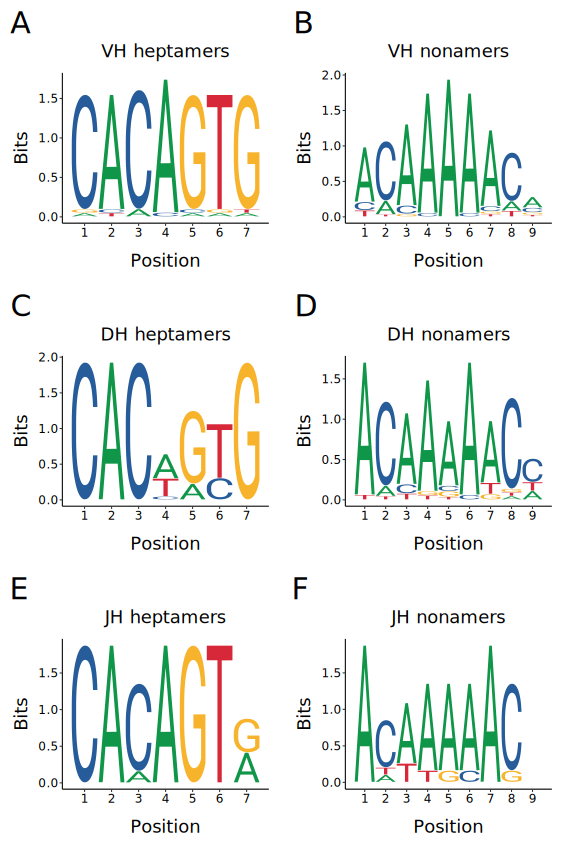
\includegraphics[width=0.9\textwidth]{_Figures/png/nfu-rss-seqlogo-sep}
	\caption[\Nfu recombination signal sequences by segment type]{\textbf{\Nfu recombination signal sequences by segment type:} Sequence composition of conserved heptamer (A,C,E) and nonamer (B,D,F) sequences from \Nfu heavy-chain RSSs associated with \vh (A,B), \dh (C,D) or \jh (E,F) gene segments.}
	\label{fig:nfu-rss-seqlogo-sep}
\end{figure}

\begin{figure}
	\centering
	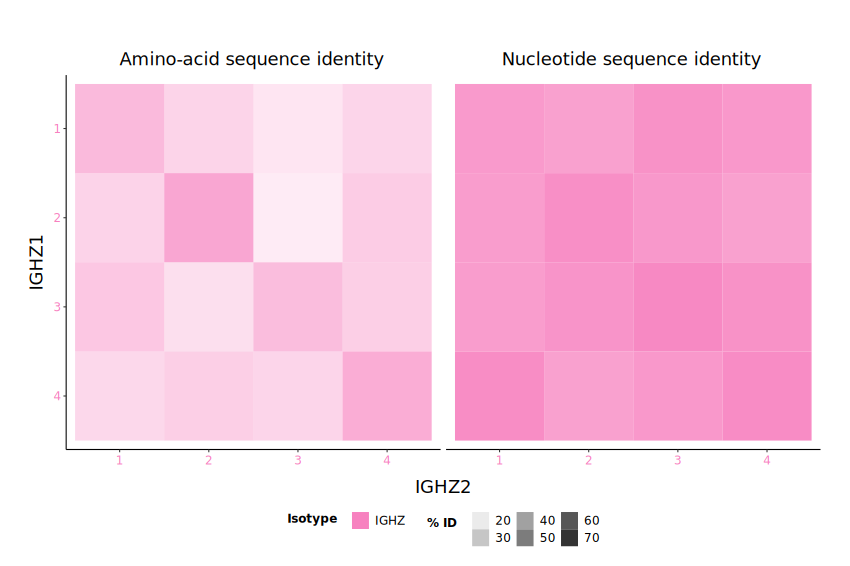
\includegraphics[width=0.8\textwidth]{_Figures/png/xma-new-cz-aln}
	\caption[Sequence similarity between \igh{Z} constant-regions in \Xma]{\textbf{Sequence similarity between \igh{Z} constant-regions in \Xma:} Heatmap of percentage sequence identity between amino-acid (right) and nucleotide (left) sequences of \cz{} exons from the two \Xma \igh{Z} constant regions, calculated using pairwise Needleman-Wunsch global alignments.} % TODO: Combine isotype and identity legends
	\label{fig:xma-cz-aln}
\end{figure}

	\begin{figure}
	\centering
	\includegraphics[width=\textwidth]{_Figures/png/xma-vh-families-map}
	\caption[Heatmap of \vh families in the in \Xma \textit{IgH} locus]{\textbf{Heatmap of \vh families in the in \Xma (\textit{IgH}) locus:} Heatmap of family relationships among \Xma \vh segments, with coloured shading indicating families and red dots indicating pairwise nucleotide sequence identity of at least 80\%. \vh families containing multiple segments are uniquely coloured, while single-segment families are in grey.}
	\label{fig:xma-vh-families-map}
	\end{figure}

	\begin{figure}
	\centering
	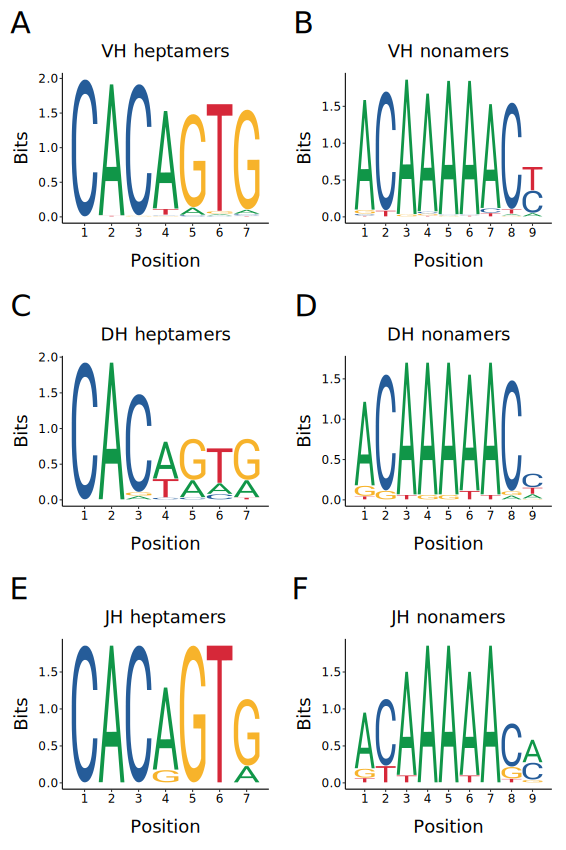
\includegraphics[width=0.9\textwidth]{_Figures/png/xma-new-rss-seqlogo-sep}
	\caption[\Xma recombination signal sequences by segment type]{\textbf{\Xma recombination signal sequences by segment type:} Sequence composition of conserved heptamer (A,C,E) and nonamer (B,D,F) sequences from \Xma heavy-chain RSSs associated with \vh (A,B), \dh (C,D) or \jh (E,F) gene segments.}
	\label{fig:xma-rss-seqlogo-sep}
	\end{figure}
\chapter{Supplementary tables}
\label{app:tables}

\begin{table}
\caption{Software versions used in computational analyses}
\label{tab:software-versions}
\centering
% latex table generated in R 3.5.2 by xtable 1.8-3 package
% Sun Mar 17 19:16:12 2019
\begin{tabular}{ll}
  \toprule Program & Version \\ 
  \midrule Basemount & 0.15.96.2154 \\ 
  BLAST & 2.7.1 \\ 
  Bowtie 2 & 2.2.6 \\ 
  CD-HIT-EST & 4.6.8 \\ 
  Change-O & 0.4.5 \\ 
  EMBOSS (FUZZNUC) & 6.6.0 \\ 
  FigTree & 1.4.2 \\ 
  HMMER & 3.2 \\ 
  IgBLAST & 1.7.0 \\ 
  IGoR & 1.3.0 \\ 
  IGV & 2.3.68 \\ 
  IMGT/DomainGapAlign & 4.9.2 \\ 
  PRANK & v.170427 \\ 
  pRESTO & 0.5.10 \\ 
  Primer3 & 2.3.6 \\ 
  Python 2 & 2.7.14 \\ 
  Python 3 & 3.6.4 \\ 
  QuorUM & 1.0.0 \\ 
  R & 3.4.1/3.5.2 \\ 
  RAxML & 8.2.12 \\ 
  RepeatMasker & 4.0.6 \\ 
  SAMtools & 1.9 \\ 
  sed & 4.2.2 \\ 
  seqtk & 1.3 \\ 
  Snakemake & 5.3.0 \\ 
  SPAdes & 3.6.1 \\ 
  SSPACE & 3.0 \\ 
  STAR & 2.5.2b \\ 
  Trimmomatic & 0.32 \\ 
  VSEARCH & 2.8.0 \\ 
   \bottomrule \end{tabular}

\end{table}

\begin{table}
\caption{RNA-sequencing datasets used for \textit{IGH} locus characterisation}
\centering
\begin{threeparttable}
\begin{tabular}{>{\bfseries}c|c|c}\toprule
Species & \Nfu & \Xma \\\midrule
Tissues & Gut & Various\tnote{a}\\\midrule
BioProject Accession & PRJNA379208 & PRJNA420092\\\midrule
\multirow{26}{*}{SRA Run Accessions} & SRR5344350 & SRR6327069\\
& SRR5344343 & SRR6327070\\
& SRR5344344 & SRR6327071\\
& SRR5344345 & SRR6327072\\
& SRR5344346 & SRR6327073\\
& SRR5344347 & SRR6327074\\
& SRR5344348 & SRR6327075\\
& SRR5344349 & SRR6327076\\
& SRR5344350 & SRR6327077\\
&&SRR6327078\\
&&SRR6327079\\
&&SRR6327080\\
&&SRR6327081\\
&&SRR6327082\\
&&SRR6327083\\
&&SRR6327084\\
&&SRR6327085\\
&&SRR6327086\\
&&SRR6327087\\
&&SRR6327088\\
&&SRR6327089\\
&&SRR6327090\\
&&SRR6327091\\
&&SRR6327092\\
&&SRR6327093\\
&&SRR6327094\\\midrule
Source & \parencite{smith2017microbiota} & Citation not given\\
\bottomrule\end{tabular}
	\begin{tablenotes}
	\item[a] Tissues used for \Xma RNA-sequencing included brain, heart, liver, gut, skin or whole fish; see BioProject entry for details.
	\end{tablenotes}
\end{threeparttable}
\label{tab:rnaseq-sources}
\end{table}

% 3 - LOCUS CHAPTER
\centering

\begin{table}\centering
    \caption{Co-ordinate table of constant-region exons in the \Nfu \igh{} locus}
    	% latex table generated in R 3.5.2 by xtable 1.8-3 package
% Tue Jan 15 17:07:52 2019
\begin{tabular}{llrrrl}
  \toprule Name & Isotype & Start & End & Length & Strand \\ 
  \midrule IGH1M-1 & M & 130848 & 131144 & 297 & + \\ 
  IGH1M-2 & M & 131971 & 132312 & 342 & + \\ 
  IGH1M-3 & M & 132394 & 132705 & 312 & + \\ 
  IGH1M-4 & M & 132816 & 133288 & 473 & + \\ 
  IGH1M-TM1 & M & 134262 & 134413 & 152 & + \\ 
  IGH1M-TM2 & M & 138431 & 138819 & 389 & + \\ 
  IGH1D-1 & D & 139381 & 139689 & 309 & + \\ 
  IGH1D-2A & D & 139774 & 140064 & 291 & + \\ 
  IGH1D-3A & D & 140178 & 140489 & 312 & + \\ 
  IGH1D-4A & D & 140572 & 140853 & 282 & + \\ 
  IGH1D-2B & D & 145613 & 145909 & 297 & + \\ 
  IGH1D-3B & D & 146000 & 146311 & 312 & + \\ 
  IGH1D-4B & D & 146398 & 146676 & 279 & + \\ 
  IGH1D-5 & D & 146795 & 147124 & 330 & + \\ 
  IGH1D-6 & D & 147210 & 147527 & 318 & + \\ 
  IGH1D-7 & D & 147598 & 147885 & 288 & + \\ 
  IGH1D-TM1 & D & 148016 & 148164 & 149 & + \\ 
  IGH1D-TM2 & D & 148323 & 148504 & 182 & + \\ 
  IGH2D-TM2 & D & 187624 & 187803 & 180 & - \\ 
  IGH2D-TM1 & D & 187963 & 188111 & 149 & - \\ 
  IGH2D-7 & D & 188658 & 188945 & 288 & - \\ 
  IGH2D-6 & D & 189016 & 189333 & 318 & - \\ 
  IGH2D-5 & D & 189419 & 189748 & 330 & - \\ 
  IGH2D-4B & D & 189867 & 190145 & 279 & - \\ 
  IGH2D-3B & D & 190232 & 190543 & 312 & - \\ 
  IGH2D-2B & D & 190636 & 190932 & 297 & - \\ 
  IGH2D-4A & D & 195644 & 195925 & 282 & - \\ 
  IGH2D-3A & D & 196008 & 196319 & 312 & - \\ 
  IGH2D-2A & D & 196433 & 196723 & 291 & - \\ 
  IGH2D-1 & D & 196808 & 197116 & 309 & - \\ 
  IGH2M-TM2 & M & 198315 & 198506 & 192 & - \\ 
  IGH2M-TM1 & M & 199834 & 199985 & 152 & - \\ 
  IGH2M-4 & M & 200953 & 201425 & 473 & - \\ 
  IGH2M-3 & M & 201536 & 201847 & 312 & - \\ 
  IGH2M-2 & M & 201929 & 202270 & 342 & - \\ 
  IGH2M-1 & M & 203549 & 203845 & 297 & - \\ 
   \bottomrule \end{tabular}

    \label{tab:nfu-ch-coords}
\end{table}

    \begin{landscape}
        \centering
        \vspace*{\fill}
        \scriptsize
		% latex table generated in R 3.5.2 by xtable 1.8-3 package
% Fri Jan  4 11:18:28 2019
\begin{tabular}{lrrrlrlrlrrl}
  \toprule Name & Start & End & Length & Strand & RSS Start & Heptamer & Spacer Length & Nonamer & RSS End & RSS Length & Comment \\ 
  \midrule IGH1V1-01 & 1252 & 1540 & 289 & + & 1541 & CACAGTG & 22 & ACAAAAACC & 1578 & 38 &  \\ 
  IGH1V1-02 & 3365 & 3656 & 292 & + & 3657 & CACAGTG & 22 & ACAAAAACC & 3694 & 38 &  \\ 
  IGH1V2-01 & 5907 & 6201 & 295 & + & 6202 & CACAGAA & 15 & ACAAAAACT & 6232 & 31 &  \\ 
  IGH1V1-03 & 13690 & 13964 & 275 & + & 13965 & CACAGTG & 22 & ACAAAAACC & 14002 & 38 &  \\ 
  IGH1V3-01 & 14862 & 15162 & 301 & + & 15163 & CACAGTG & 23 & ACAAAAACC & 15201 & 39 &  \\ 
  IGH1V2-02 & 17433 & 17730 & 298 & + & 17731 & CACAATG & 23 & ACAAAAACC & 17769 & 39 &  \\ 
  IGH1V4-01 & 24566 & 24837 & 272 & + & 24838 & CGCAGTG & 22 & CCACAAACC & 24875 & 38 & Nonsense mutation \\ 
  IGH1V1-04 & 37305 & 37596 & 292 & + & 37597 & CACAGTG & 22 & ACAAAAACC & 37634 & 38 &  \\ 
  IGH1V2-03 & 48845 & 49139 & 295 & + & 49140 & CACAGTG & 23 & TCAAAAACT & 49178 & 39 &  \\ 
  IGH1V1-05 & 49909 & 50197 & 289 & + & 50198 & CACAGTG & 22 & ACAAAAACC & 50235 & 38 &  \\ 
  IGH1V5-01 & 51710 & 51998 & 289 & + & 51999 & CACAGTG & 22 & ACAAAAACT & 52036 & 38 &  \\ 
  IGH1V2-04 & 56322 & 56616 & 295 & + & 56617 & CACAGTG & 23 & ACAAAAACC & 56655 & 39 &  \\ 
  IGH1V6-01 & 57465 & 57762 & 298 & + & 57763 & CACAGTG & 21 & ACTAAATCT & 57799 & 37 &  \\ 
  IGH1V1-06 & 59678 & 59966 & 289 & + & 59967 & CACAGTG & 22 & ACAAAAACC & 60004 & 38 &  \\ 
  IGH1V4-02 & 68017 & 68288 & 272 & + & 68289 & TGCAGTG & 22 & TCACAAACC & 68326 & 38 & Nonsense mutation \\ 
  IGH1V2-05 & 69787 & 70084 & 298 & + & 70085 & CACAGTG & 23 & ACAAAAACC & 70123 & 39 &  \\ 
  IGH1V1-07 & 155485 & 155763 & 279 & + & 155764 & CACAGTG & 22 & TCAAAACCC & 155801 & 38 &  \\ 
  IGH2V2-02 & 282620 & 282914 & 295 & - & 282915 & CACAGTG & 23 & ACAAAAACC & 282953 & 39 &  \\ 
  IGH2V4-01 & 284404 & 284675 & 272 & - & 284676 & TGCAGTG & 22 & TCACAAACC & 284713 & 38 & Nonsense mutation \\ 
  IGH2V5-01 & 288808 & 289096 & 289 & - & 289097 & CACAGTG & 22 & ACAGAAACT & 289134 & 38 &  \\ 
  IGH2V1-03 & 289977 & 290271 & 295 & - & 290272 & CACAGTG & 22 & ACAAAAACC & 290309 & 38 &  \\ 
  IGH2V1-02 & 293835 & 294126 & 292 & - & 294127 & CACAGTG & 22 & ACAAAAACC & 294164 & 38 &  \\ 
  IGH2V2-01 & 303780 & 304074 & 295 & - & 304075 & CAGGGCC & 24 & AGCACAAAG & 304114 & 40 &  \\ 
  IGH2V1-01 & 304926 & 305204 & 279 & - & 305205 & CACAGTG & 22 & TCAAAACCC & 305242 & 38 &  \\ 
   \bottomrule \end{tabular}

		\normalsize\vspace{1em}
        \captionof{table}{Co-ordinate table of \vh segments in the \Nfu \igh{} locus}
        \label{tab:nfu-vh-coords}
        \vspace*{\fill}
    \end{landscape}

        {\centering
        \captionof{table}{Co-ordinate table of \dh segments in the \Nfu \igh{} locus}\vspace{-0.3em}
        \label{tab:nfu-dh-coords-seg}
        \scriptsize
		% latex table generated in R 3.5.2 by xtable 1.8-3 package
% Tue Jan 15 17:07:52 2019
\begin{tabular}{lrlrrl}
  \toprule Name & Start & NT Sequence & End & Length & Strand \\ 
  \midrule IGH1D01 & 25782 & ATACGTACTTTCGTGGTATATAGAGA & 25807 & 26 & + \\ 
  IGH1D02 & 76700 & GATATCTGGGTGGGGG & 76715 & 16 & + \\ 
  IGH1D03 & 77027 & TGAAATGATTAC & 77038 & 12 & + \\ 
  IGH1D04 & 77476 & TCGCGTAGCGGC & 77487 & 12 & + \\ 
  IGH1D05 & 78717 & GAAACCACGGCAGC & 78730 & 14 & + \\ 
  IGH1D06 & 79049 & TTTATAGCGGCTAC & 79062 & 14 & + \\ 
  IGH1D07 & 80417 & CAGACTGGAGA & 80427 & 11 & + \\ 
  IGH1D08 & 81362 & TTCATGGCAGCCAC & 81375 & 14 & + \\ 
  IGH1D09 & 82067 & CAGACTGGAGC & 82077 & 11 & + \\ 
  IGH1D10 & 84282 & TGGGGTGGCAGC & 84293 & 12 & + \\ 
  IGH2D04 & 263497 & CAGACTGGAGA & 263507 & 11 & - \\ 
  IGH2D03 & 270243 & TTTATAGCGGCTAC & 270256 & 14 & - \\ 
  IGH2D02 & 270878 & GAAACCACGGCAGC & 270891 & 14 & - \\ 
  IGH2D01 & 271749 & GACTTTTACTAC & 271760 & 12 & - \\ 
   \bottomrule \end{tabular}

		\normalsize\vspace{1em}
        \captionof{table}{Co-ordinate table of \dh 5'-RSSs in the \Nfu \igh{} locus}\vspace{-0.3em}
        \label{tab:nfu-dh-coords-rss5}
        \scriptsize
        	% latex table generated in R 3.5.2 by xtable 1.8-3 package
% Fri Jan  4 11:18:28 2019
\begin{tabular}{lrlrlrr}
  \toprule Name & 5'-RSS Start & Nonamer & Spacer Length & Heptamer & 5'-RSS End & Length \\ 
  \midrule IGH1D01 & 25754 & GGTTGTTGT & 12 & CACTGTG & 25781 & 28 \\ 
  IGH1D02 & 76672 & AGTTTTTGA & 12 & CACAGTG & 76699 & 28 \\ 
  IGH1D03 & 76999 & TGTTGTTGT & 12 & CACAGTG & 77026 & 28 \\ 
  IGH1D04 & 77448 & AGTTTTTGT & 12 & CACGGTG & 77475 & 28 \\ 
  IGH1D05 & 78688 & GATGTTTTT & 13 & CACAGTG & 78716 & 29 \\ 
  IGH1D06 & 79021 & TGTTTTTGT & 12 & CGCTGTG & 79048 & 28 \\ 
  IGH1D07 & 80417 & AGTTTTGGT & 12 & CACAGTG & 80444 & 28 \\ 
  IGH1D08 & 81334 & TGTTTTTGT & 12 & CGCTGTG & 81361 & 28 \\ 
  IGH1D09 & 82039 & AGTTTTGGT & 12 & CACAGTG & 82066 & 28 \\ 
  IGH1D10 & 84254 & TCATTCATT & 12 & CACTGTG & 84281 & 28 \\ 
  IGH2D04 & 263497 & AGTTTTGGT & 12 & CACAGTG & 263524 & 28 \\ 
  IGH2D03 & 270215 & TGTTTTTGT & 12 & CGCTGTG & 270242 & 28 \\ 
  IGH2D02 & 270850 & TGTTTTTGT & 12 & CACAGTG & 270877 & 28 \\ 
  IGH2D01 & 271721 & AGTTTTTAT & 12 & CATGGTG & 271748 & 28 \\ 
   \bottomrule \end{tabular}

        	\normalsize\vspace{1em}
        \captionof{table}{Co-ordinate table of \dh 3'-RSSs in the \Nfu \igh{} locus}\vspace{-0.3em}
        \label{tab:nfu-dh-coords-rss3}
        \scriptsize
		% latex table generated in R 3.5.2 by xtable 1.8-3 package
% Tue Jan 15 17:07:52 2019
\begin{tabular}{lrlrlrr}
  \toprule Name & 3'-RSS Start & Heptamer & Spacer Length & Nonamer & 3'-RSS End & Length \\ 
  \midrule IGH1D01 & 25808 & CACAGTG & 12 & ACAAAAACC & 25835 & 28 \\ 
  IGH1D02 & 76716 & CACAGTG & 12 & ACAAAAACC & 76743 & 28 \\ 
  IGH1D03 & 77039 & CACTGTG & 11 & AATATAACC & 77065 & 27 \\ 
  IGH1D04 & 77488 & CACAGCG & 12 & ACATAAAAC & 77515 & 28 \\ 
  IGH1D05 & 78731 & CACAGCG & 12 & ACAAAAGCC & 78758 & 28 \\ 
  IGH1D06 & 79063 & CACTGTG & 12 & ACAAGATCC & 79090 & 28 \\ 
  IGH1D07 & 80428 & CACAACG & 12 & ACAAAAACC & 80455 & 28 \\ 
  IGH1D08 & 81376 & CACTGTG & 12 & ACAAAATCC & 81403 & 28 \\ 
  IGH1D09 & 82078 & CACAATG & 12 & ACAAAAACC & 82105 & 28 \\ 
  IGH1D10 & 84294 & CACAGTG & 12 & ACAAAAACC & 84321 & 28 \\ 
  IGH2D04 & 263508 & CACAACG & 12 & ACAAAAACC & 263535 & 28 \\ 
  IGH2D03 & 270257 & CACTGTG & 12 & ACAAGATCC & 270284 & 28 \\ 
  IGH2D02 & 270892 & CACAGCG & 12 & ACAAAAGCC & 270919 & 28 \\ 
  IGH2D01 & 271761 & CACAATG & 12 & ACAAAAACC & 271788 & 28 \\ 
   \bottomrule \end{tabular}

		\normalsize
		}

    \begin{landscape}
        \centering
        \notsotiny
		% latex table generated in R 3.5.2 by xtable 1.8-3 package
% Tue Jan 15 17:07:52 2019
\begin{tabular}{lrllrrl}
  \toprule Name & Start & NT Sequence & AA Sequence & End & Length & Strand \\ 
  \midrule IGH1J01 & 26187 & GTGCTTTAGACAACTGGGGAAAAGGAACGGAGGTTACTGTTCAACCTG & ALDNWGKGTEVTVQP & 26234 & 48 & + \\ 
  IGH1J02 & 128176 & ATGACTACTTTGACTACTGGGGAAAAGGAACAATGGTGACGGTCACATCAG & DYFDYWGKGTMVTVTS & 128226 & 51 & + \\ 
  IGH1J03 & 128354 & ACCGTGGGGTAAAGGGACAACAGTCACGGTCAAAACAG & PWGKGTTVTVKT & 128391 & 38 & + \\ 
  IGH1J04 & 128533 & ACGGTGCTCTTGACTACTGGGGTAAAGGGACCGCAGTCACTGTAACATCAG & GALDYWGKGTAVTVTS & 128583 & 51 & + \\ 
  IGH1J05 & 128887 & ACAACGCTTTTGACTACTGGGGAAAAGGAACAACGGTCACCGTCACTTCAG & NAFDYWGKGTTVTVTS & 128937 & 51 & + \\ 
  IGH1J06 & 129346 & CTACGATGCTTTTGACTACTGGGGGAAAAGGACGATGGTCACGTCACTTCAG & YDAFDYWGKRTMVTSLQ & 129397 & 52 & + \\ 
  IGH1J07 & 129635 & TTAACTGGGCTTTCGACTACTGGGGAAAAGGGACGATGGTAACGGTGACTTCAG & NWAFDYWGKGTMVTVTS & 129688 & 54 & + \\ 
  IGH1J08 & 129965 & TTACCACGCAGCTTTGGACTACTGGGGAAAAGGGACGACGGTCACCGTCACCTCAG & YHXALDYWGKGTTVTVTS & 130020 & 56 & + \\ 
  IGH1J09 & 130612 & TCTACGCTGCTTTTGACTACTGGGGTAAAGGTACAACGGTAACCGTTTCATCAG & YAAFDYWGKGTTVTVSS & 130665 & 54 & + \\ 
  IGH2J08 & 204031 & TCTACGCTGCTTTTGACTACTGGGGTAAAGGTACAACGGTAACCGTTTCATCAG & YAAFDYWGKGTTVTVSS & 204084 & 54 & - \\ 
  IGH2J07 & 204673 & TTACCACGCAGCTTTGGACTACTGGGGAAAAGGGACGACGGTCACCGTCACCTCAG & YHXALDYWGKGTTVTVTS & 204728 & 56 & - \\ 
  IGH2J06 & 205005 & ATAACTGGGCTTTCGACTACTGGGGAAAAGGGACGATGGTAACGGTGACTTCAG & NWAFDYWGKGTMVTVTS & 205058 & 54 & - \\ 
  IGH2J05 & 205296 & CTACGATGCTTTTGACTACTGGGGGAAAAGGACGATGGTCACGTCACTTCAG & YDAFDYWGKRTMVTSLQ & 205347 & 52 & - \\ 
  IGH2J04 & 205756 & ACAACGCTTTTGACTACTGGGGAAAAGGAACAACGGTCACCGTCACTTCAG & NAFDYWGKGTTVTVTS & 205806 & 51 & - \\ 
  IGH2J03 & 206111 & ATGGTGCTTTTGACTACTGGGGTAAAGGGACCGCAGTCACTGTAACATCAG & GAFDYWGKGTAVTVTS & 206161 & 51 & - \\ 
  IGH2J02 & 206303 & ACCGTGGGGTAAAGGGACAACAGTCACGGTCAAAACAG & PWGKGTTVTVKT & 206340 & 38 & - \\ 
  IGH2J01 & 206466 & ATGACTACTTTGACTACTGGGGAAAAGGAACAATGGTGACGGTCACATCAG & DYFDYWGKGTMVTVTS & 206516 & 51 & - \\ 
   \bottomrule \end{tabular}

		\normalsize\vspace{0.6em}
        \captionof{table}{Co-ordinate table of \jh segments in the \Nfu \igh{} locus}
        \label{tab:nfu-jh-coords-seg}
        \notsotiny
		% latex table generated in R 3.5.2 by xtable 1.8-3 package
% Tue Jan 15 17:07:52 2019
\begin{tabular}{lrlrlrr}
  \toprule Name & RSS Start & Nonamer & Spacer Length & Heptamer & RSS End & RSS Length \\ 
  \midrule IGH1J01 & 26196 & TGTTTTTGT & 23 & CACTGTG & 26186 & 39 \\ 
  IGH1J02 & 128188 & AGTGTTTGT & 23 & CACTGTG & 128175 & 39 \\ 
  IGH1J03 & 128353 & TGTTTATTT & 23 & CACTGTG & 128353 & 39 \\ 
  IGH1J04 & 128545 & GGTTTTTGT & 23 & CACTGTG & 128532 & 39 \\ 
  IGH1J05 & 128899 & GGTTTTAGT & 23 & TACTGTG & 128886 & 39 \\ 
  IGH1J06 & 129360 & TCTTCTTGT & 22 & TACTTTG & 129345 & 38 \\ 
  IGH1J07 & 129650 & AGTTTTTGT & 23 & TACTGTG & 129634 & 39 \\ 
  IGH1J08 & 129983 & AGTTTTAGT & 22 & TACTGTG & 129964 & 38 \\ 
  IGH1J09 & 130628 & CGTTTTTAT & 22 & CACTGTG & 130611 & 38 \\ 
  IGH2J08 & 204047 & CGTTTTTAT & 22 & CACTGTG & 204030 & 38 \\ 
  IGH2J07 & 204691 & AGTTTTAGT & 22 & TACTGTG & 204672 & 38 \\ 
  IGH2J06 & 205020 & AGTTTTTGT & 23 & TACTGTG & 205004 & 39 \\ 
  IGH2J05 & 205310 & TCTTCTTGT & 22 & TACTTTG & 205295 & 38 \\ 
  IGH2J04 & 205768 & GGTTTTAGT & 23 & TACTGTG & 205755 & 39 \\ 
  IGH2J03 & 206123 & GGTTTTTGT & 23 & CACTGTG & 206110 & 39 \\ 
  IGH2J02 & 206302 & TGTTTATTT & 23 & CACTGTG & 206302 & 39 \\ 
  IGH2J01 & 206478 & AGTGTTTGT & 23 & CACTGTG & 206465 & 39 \\ 
   \bottomrule \end{tabular}

		\normalsize\vspace{0.6em}
        \captionof{table}{Co-ordinate table of \jh RSSs in the \Nfu \igh{} locus}
        \label{tab:nfu-jh-coords-rss}
    \end{landscape}

\begin{table}\centering
    \caption{Co-ordinate table of constant-region exons in the \Xma \igh{} locus}
    	% latex table generated in R 3.5.2 by xtable 1.8-3 package
% Tue Jan  8 15:33:35 2019
\begin{tabular}{llrrrl}
  \toprule Name & Isotype & Start & End & Length & Strand \\ 
  \midrule IGHZ1-1 & Z & 3380 & 3667 & 288 & + \\ 
  IGHZ1-2 & Z & 3814 & 4098 & 285 & + \\ 
  IGHZ1-3 & Z & 4195 & 4497 & 303 & + \\ 
  IGHZ1-4 & Z & 4934 & 5263 & 330 & + \\ 
  IGHZ1-S & Z & 5264 & 5459 & 196 & + \\ 
  IGHZ1-TM1 & Z & 6345 & 6490 & 146 & + \\ 
  IGHZ1-TM2 & Z & 6645 & 7043 & 399 & + \\ 
  IGHZ2-1 & Z & 256059 & 256337 & 279 & + \\ 
  IGHZ2-2 & Z & 256453 & 256734 & 282 & + \\ 
  IGHZ2-3 & Z & 256893 & 257171 & 279 & + \\ 
  IGHZ2-4 & Z & 257319 & 257636 & 318 & + \\ 
  IGHZ2-S & Z & 257637 & 257850 & 214 & + \\ 
  IGHZ2-TM1 & Z & 258059 & 258213 & 155 & + \\ 
  IGHZ2-TM2 & Z & 258410 & 258629 & 220 & + \\ 
  IGHM-1 & M & 279664 & 279960 & 297 & + \\ 
  IGHM-2 & M & 280880 & 281224 & 345 & + \\ 
  IGHM-3 & M & 281321 & 281629 & 309 & + \\ 
  IGHM-4 & M & 281789 & 282291 & 503 & + \\ 
  IGHM-TM1 & M & 282910 & 283034 & 125 & + \\ 
  IGHM-TM2 & M & 285028 & 285740 & 713 & + \\ 
  IGHD-1 & D & 285902 & 286219 & 318 & + \\ 
  IGHD-2A & D & 286310 & 286597 & 288 & + \\ 
  IGHD-3A & D & 286814 & 287128 & 315 & + \\ 
  IGHD-4A & D & 287250 & 287534 & 285 & + \\ 
  IGHD-2B & D & 288876 & 289166 & 291 & + \\ 
  IGHD-3B & D & 289262 & 289576 & 315 & + \\ 
  IGHD-4B & D & 289680 & 289964 & 285 & + \\ 
  IGHD-5 & D & 290052 & 290381 & 330 & + \\ 
  IGHD-6 & D & 290472 & 290789 & 318 & + \\ 
  IGHD-7 & D & 290865 & 291152 & 288 & + \\ 
  IGHD-TM1 & D & 291286 & 291434 & 149 & + \\ 
  IGHD-TM2 & D & 291541 & 291642 & 102 & + \\ 
   \bottomrule \end{tabular}

    \label{tab:xma-ch-coords}
\end{table}

    \begin{landscape}
        \centering
        \vspace*{\fill}
        \scriptsize
		% latex table generated in R 3.5.2 by xtable 1.8-3 package
% Tue Jan  8 15:33:33 2019
\begin{tabular}{lrrrlrlllrrl}
  \toprule Name & Start & End & Length & Strand & RSS Start & Heptamer & Spacer Length & Nonamer & RSS End & RSS Length & Comment \\ 
  \midrule IGHV01-01 & 1159 & 1450 & 292 & + & 1451 & CACAGTG & 23 & GTAAAAACC & 1489 & 39 &  \\ 
  IGHV02-01 & 10534 & 10825 & 292 & + & 10826 & CACAGTG & 23 & ACAAAACCC & 10864 & 39 &  \\ 
  IGHV02-02 & 11961 & 12261 & 301 & + & 12262 & CACTGTG & 23 & ACAAAAACT & 12300 & 39 &  \\ 
  IGHV02-03 & 13319 & 13616 & 298 & + & 13617 & CACAGTG & 23 & ACACAAACT & 13655 & 39 &  \\ 
  IGHV03-01 & 15440 & 15734 & 295 & + & 15735 & CACAGTG & 22 & ACAAAAACT & 15772 & 38 &  \\ 
  IGHV02-04 & 16618 & 16908 & 291 & + & 16909 & CACAGTG & 23 & ACAAAAACC & 16947 & 39 &  \\ 
  IGHV02-05 & 17522 & 17822 & 301 & + & 17823 & CACTGTG & 22 & ACAAAAACT & 17860 & 38 &  \\ 
  IGHV02-06 & 18881 & 19178 & 298 & + & 19179 & CACAGTG & 23 & ACACAAACT & 19217 & 39 &  \\ 
  IGHV03-02 & 21000 & 21294 & 295 & + & 21295 & CACAGTG & 22 & ACAAAAACT & 21332 & 38 &  \\ 
  IGHV02-07 & 22179 & 22467 & 289 & + & 22468 & CACAGTG & 23 & ACAAAAACC & 22506 & 39 &  \\ 
  IGHV02-08p & 24234 & 24514 & 281 & + & 24515 & CACAGTG & 23 & ACAAAAACT & 24553 & 39 & Frameshift \\ 
  IGHV04-01 & 25359 & 25659 & 301 & + & 25660 & CACAGTG & 23 & ACAAAAACT & 25698 & 39 &  \\ 
  IGHV04-02 & 27066 & 27366 & 301 & + & 27367 & CACAGTG & 23 & ACAAAAACA & 27405 & 39 &  \\ 
  IGHV02-09 & 28669 & 28958 & 290 & + & 28959 & CACAGTG & 23 & ACAAAAACC & 28997 & 39 &  \\ 
  IGHV02-10p & 30460 & 30741 & 282 & + & 30742 & CACAATG & 23 & ACAAAACTC & 30780 & 39 & Frameshift \\ 
  IGHV02-11 & 32395 & 32681 & 287 & + & 32682 & CACAGTG & 23 & ACAAAAACC & 32720 & 39 &  \\ 
  IGHV03-03 & 33663 & 33957 & 295 & + & 33958 & CACTGTG & 22 & ACAAAAACT & 33995 & 38 &  \\ 
  IGHV02-12 & 35012 & 35299 & 288 & + & 35300 & CACAGTG & 23 & ACAAAAACC & 35338 & 39 &  \\ 
  IGHV03-04 & 36281 & 36575 & 295 & + & 36576 & CACTGTG & 22 & ACAAAAACT & 36613 & 38 &  \\ 
  IGHV02-13 & 37639 & 37931 & 293 & + & 37932 & CACAGTG & 23 & ACAAAAACT & 37970 & 39 &  \\ 
  IGHV02-14 & 39019 & 39311 & 293 & + & 39312 & CACAGTG & 23 & ACAAAAACT & 39350 & 39 &  \\ 
  IGHV03-05 & 41008 & 41302 & 295 & + & 41303 & CACAGTG & 22 & ACAAAAACT & 41340 & 38 &  \\ 
  IGHV02-15 & 42660 & 42952 & 293 & + & 42953 & CACAGTG & 23 & ACAAAAACT & 42991 & 39 &  \\ 
  IGHV03-06 & 45081 & 45375 & 295 & + & 45376 & CACAGTG & 22 & ACAAAAACT & 45413 & 38 &  \\ 
  IGHV02-16 & 46732 & 47024 & 293 & + & 47025 & CACAGTG & 23 & ACAAAAACT & 47063 & 39 &  \\ 
   \bottomrule \end{tabular}

		\normalsize\vspace{1em}
        \captionof{table}{Co-ordinate table of \vh segments in the \Xma \igh{} locus, part 1}
        \label{tab:xma-vh-coords-1}
        \vspace*{\fill}
    \end{landscape}

    \begin{landscape}
        \centering
        \vspace*{\fill}
        \scriptsize
		% latex table generated in R 3.5.2 by xtable 1.8-3 package
% Tue Jan  8 15:33:33 2019
\begin{tabular}{lrrrlrlllrrl}
  \toprule Name & Start & End & Length & Strand & RSS Start & Heptamer & Spacer Length & Nonamer & RSS End & RSS Length & Comment \\ 
  \midrule IGHV03-07 & 48618 & 48912 & 295 & + & 48913 & CACAGTG & 22 & ACAAAAACT & 48950 & 38 &  \\ 
  IGHV02-17 & 50323 & 50611 & 289 & + & 50612 & CACAGTG & 23 & ACAAAAACC & 50650 & 39 &  \\ 
  IGHV03-08 & 51890 & 52184 & 295 & + & 52185 & CACAGTG & 22 & ACAAAAACT & 52222 & 38 &  \\ 
  IGHV03-09p & 53026 & 53274 & 249 & + & 53275 &  &  &  &  &  & 3'-truncated, no RSS \\ 
  IGHV02-18 & 54462 & 54747 & 286 & + & 54748 & CACAGTG & 23 & ACAAAAACC & 54786 & 39 &  \\ 
  IGHV02-19p & 55729 & 55866 & 138 & + & 55867 & CACAGTG & 23 & ACAAAAACC & 55905 & 39 & 3'-truncated \\ 
  IGHV03-10 & 57371 & 57662 & 292 & + & 57663 & CACAGTG & 22 & ACAAAAACT & 57700 & 38 &  \\ 
  IGHV02-20p & 58698 & 58986 & 289 & + & 58987 & CACAGTG & 23 & ATAAAAACC & 59025 & 39 & Nonsense mutation \\ 
  IGHV03-11 & 59940 & 60234 & 295 & + & 60235 & CACAGTG & 22 & ACAAAAACT & 60272 & 38 &  \\ 
  IGHV02-21 & 61249 & 61537 & 289 & + & 61538 & CACAGTG & 23 & ATAAAAACC & 61576 & 39 &  \\ 
  IGHV03-12 & 62491 & 62785 & 295 & + & 62786 & CACAGTG & 22 & ACAAAAACT & 62823 & 38 &  \\ 
  IGHV02-22 & 63801 & 64089 & 289 & + & 64090 & CACAGTG & 23 & ATAAAAACC & 64128 & 39 &  \\ 
  IGHV03-13 & 65043 & 65337 & 295 & + & 65338 & CACAGTG & 22 & ACAAAAACT & 65375 & 38 &  \\ 
  IGHV02-23 & 66354 & 66640 & 287 & + & 66641 & CACAGTG & 23 & ACAAAAACT & 66679 & 39 &  \\ 
  IGHV03-14 & 68452 & 68743 & 292 & + & 68744 & CACTATG & 22 & ACAAAACTC & 68781 & 38 &  \\ 
  IGHV02-24 & 70101 & 70389 & 289 & + & 70390 & CACAGTG & 23 & ACAAAAACC & 70428 & 39 &  \\ 
  IGHV03-15 & 72206 & 72501 & 296 & + & 72502 & CACAGTG & 22 & ACAAAAACT & 72539 & 38 &  \\ 
  IGHV02-25 & 73484 & 73772 & 289 & + & 73773 & CACAGTG & 23 & ACAAAAACC & 73811 & 39 &  \\ 
  IGHV03-16 & 75799 & 76090 & 292 & + & 76091 & CACAGTG & 22 & ACAAAAACT & 76128 & 38 &  \\ 
  IGHV03-17 & 77773 & 78067 & 295 & + & 78068 & CACAGTG & 22 & ACAAAAACT & 78105 & 38 &  \\ 
  IGHV02-26 & 79001 & 79289 & 289 & + & 79290 & CACAGTG & 23 & ACAAAAACC & 79328 & 39 &  \\ 
  IGHV03-18 & 80492 & 80784 & 293 & + & 80785 & CACAGTG & 22 & ACAAAAACT & 80822 & 38 &  \\ 
  IGHV02-27p & 81799 & 82082 & 284 & + & 82083 & CACAGTG & 23 & ACAAAAACC & 82121 & 39 & Frameshift \\ 
  IGHV03-19 & 83736 & 84030 & 295 & + & 84031 & CACAGTG & 22 & ACAAAAACT & 84068 & 38 &  \\ 
  IGHV02-28p & 85093 & 85381 & 289 & + & 85382 & CACAGGG & 23 & GCAAAAACC & 85420 & 39 & Nonsense mutation \\ 
   \bottomrule \end{tabular}

		\normalsize\vspace{1em}
        \captionof{table}{Co-ordinate table of \vh segments in the \Xma \igh{} locus, part 2}
        \label{tab:xma-vh-coords-2}
        \vspace*{\fill}
    \end{landscape}

    \begin{landscape}
        \centering
        \vspace*{\fill}
        \scriptsize
		% latex table generated in R 3.5.2 by xtable 1.8-3 package
% Tue Jan  8 15:33:33 2019
\begin{tabular}{lrrrlrlllrrl}
  \toprule Name & Start & End & Length & Strand & RSS Start & Heptamer & Spacer Length & Nonamer & RSS End & RSS Length & Comment \\ 
  \midrule IGHV02-29 & 86225 & 86505 & 281 & + & 86506 & CACAGTG & 23 & ATAAAAACC & 86544 & 39 &  \\ 
  IGHV03-20 & 87419 & 87713 & 295 & + & 87714 & CACAGTG & 22 & ACAAAAACT & 87751 & 38 &  \\ 
  IGHV03-21 & 94532 & 94826 & 295 & + & 94827 & CACAGTG & 23 & ACAAAAACC & 94865 & 39 &  \\ 
  IGHV03-22 & 96192 & 96489 & 298 & + & 96490 & CACAGTG & 23 & ACAAAAACC & 96528 & 39 &  \\ 
  IGHV03-23 & 98068 & 98368 & 301 & + & 98369 & CACAGTG & 23 & ACAAAAACC & 98407 & 39 &  \\ 
  IGHV03-24 & 99482 & 99779 & 298 & + & 99780 & CACAGTG & 23 & ACAAAAACC & 99818 & 39 &  \\ 
  IGHV03-25 & 101639 & 101936 & 298 & + & 101937 & CACAGTG & 23 & ACAAAAACC & 101975 & 39 &  \\ 
  IGHV05-01p & 102818 & 103096 & 279 & + & 103097 & CAGAAGC & 0 & ACAAAAACT & 103112 & 16 & Frameshift \\ 
  IGHV03-26 & 104098 & 104389 & 292 & + & 104390 & CACAGTG & 23 & ACAAAATCC & 104428 & 39 &  \\ 
  IGHV06-01 & 105551 & 105831 & 281 & + & 105832 & CACAGTG & 23 & ACAAAAACC & 105870 & 39 &  \\ 
  IGHV03-27 & 107274 & 107571 & 298 & + & 107572 & CACAGTG & 23 & ACAAAAACC & 107610 & 39 &  \\ 
  IGHV03-28 & 108775 & 109072 & 298 & + & 109073 & CACAGAG & 23 & ACAAAAACC & 109111 & 39 &  \\ 
  IGHV03-29 & 110372 & 110672 & 301 & + & 110673 & CACAGTG & 23 & ACAAAAACC & 110711 & 39 &  \\ 
  IGHV07-01 & 111565 & 111856 & 292 & + & 111857 & CACAATG & 23 & ACAAAAACT & 111895 & 39 &  \\ 
  IGHV08-01p & 113033 & 113330 & 298 & + & 113331 & CACAGAG & 23 & CCAAGAACC & 113369 & 39 & Nonsense mutation \\ 
  IGHV09-01 & 115512 & 115800 & 289 & + & 115801 & CACAGTG & 22 & ACAAAAACT & 115838 & 38 &  \\ 
  IGHV10-01 & 117078 & 117379 & 302 & + & 117380 & CACAGTG & 22 & ACATAAACT & 117417 & 38 &  \\ 
  IGHV11-01 & 119462 & 119760 & 299 & + & 119761 & CACAGTG & 23 & ACAAAAACT & 119799 & 39 &  \\ 
  IGHV03-30 & 126125 & 126416 & 292 & + & 126417 & CACAGTG & 22 & ACAAAAACC & 126454 & 38 &  \\ 
  IGHV03-31 & 127109 & 127400 & 292 & + & 127401 & CACAGTG & 23 & GCAAAAACC & 127439 & 39 &  \\ 
  IGHV12-01 & 128489 & 128786 & 298 & + & 128787 & CACAGTG & 23 & ACAAAAACC & 128825 & 39 &  \\ 
  IGHV02-30 & 135711 & 136000 & 290 & + & 136001 & CACAGTG & 22 & ACAAAAACA & 136038 & 38 &  \\ 
  IGHV13-01 & 136757 & 137057 & 301 & + & 137058 & CACAGTG & 23 & ACAAAAACT & 137096 & 39 &  \\ 
  IGHV02-31 & 138344 & 138637 & 294 & + & 138638 & CACAGTG & 23 & ACAAAAATC & 138676 & 39 &  \\ 
  IGHV02-32 & 140024 & 140315 & 292 & + & 140316 & CACTGTG & 23 & ACAAAAACT & 140354 & 39 &  \\ 
   \bottomrule \end{tabular}

		\normalsize\vspace{1em}
        \captionof{table}{Co-ordinate table of \vh segments in the \Xma \igh{} locus, part 3}
        \label{tab:xma-vh-coords-3}
        \vspace*{\fill}
    \end{landscape}

    \begin{landscape}
        \centering
        \vspace*{\fill}
        \scriptsize
		% latex table generated in R 3.5.2 by xtable 1.8-3 package
% Tue Jan  8 15:33:33 2019
\begin{tabular}{lrrrlrlllrrl}
  \toprule Name & Start & End & Length & Strand & RSS Start & Heptamer & Spacer Length & Nonamer & RSS End & RSS Length & Comment \\ 
  \midrule IGHV02-33 & 142332 & 142620 & 289 & + & 142621 & CACAGTG & 23 & ACAAAAACA & 142659 & 39 &  \\ 
  IGHV02-34 & 144334 & 144625 & 292 & + & 144626 & CACAGTG & 23 & ACAAAAACT & 144664 & 39 &  \\ 
  IGHV02-35 & 145740 & 146031 & 292 & + & 146032 & CACAGTG & 23 & ACAAAAAAT & 146070 & 39 &  \\ 
  IGHV02-36 & 146903 & 147194 & 292 & + & 147195 & CACAGTG & 23 & ACAAAAACT & 147233 & 39 &  \\ 
  IGHV02-37 & 147839 & 148138 & 300 & + & 148139 & CACAGTG & 23 & ACAAAAATC & 148177 & 39 &  \\ 
  IGHV02-38p & 150504 & 150797 & 294 & + & 150798 & CACAATA & 23 & ACAAAAACC & 150836 & 39 & Nonsense mutation \\ 
  IGHV02-39 & 152249 & 152537 & 289 & + & 152538 & CACAGTA & 23 & ACAAAAACC & 152576 & 39 &  \\ 
  IGHV14-01 & 154075 & 154374 & 300 & + & 154375 & CACAGTG & 23 & ACAAAAAGT & 154413 & 39 &  \\ 
  IGHV02-40 & 155433 & 155709 & 277 & + & 155710 & CACAGTG & 23 & ACAAAAACC & 155748 & 39 &  \\ 
  IGHV02-41 & 156583 & 156870 & 288 & + & 156871 & CACAGTG & 23 & ACAAAAACC & 156909 & 39 &  \\ 
  IGHV02-42 & 163977 & 164269 & 293 & + & 164270 & CACAGTG & 23 & ACAAAACCC & 164308 & 39 &  \\ 
  IGHV03-32 & 165416 & 165708 & 293 & + & 165709 & CACAGTG & 22 & ACAAAAACA & 165746 & 38 &  \\ 
  IGHV02-43 & 166994 & 167293 & 300 & + & 167294 & CACAATG & 23 & ACAGAAACT & 167332 & 39 &  \\ 
  IGHV12-02 & 169602 & 169900 & 299 & + & 169901 & CACAGTG & 23 & ACAAAAACC & 169939 & 39 &  \\ 
  IGHV02-44 & 171452 & 171752 & 301 & + & 171753 & CACTGTG & 23 & GCAAAAACT & 171791 & 39 &  \\ 
  IGHV02-45 & 173096 & 173384 & 289 & + & 173385 & CTCAGTG & 23 & ACAAAAACC & 173423 & 39 &  \\ 
  IGHV02-46 & 174714 & 175009 & 296 & + & 175010 & CACAGTG & 23 & ACAAAAACT & 175048 & 39 &  \\ 
  IGHV02-47 & 176396 & 176697 & 302 & + & 176698 & CACAGTG & 23 & ACAAAAACT & 176736 & 39 &  \\ 
  IGHV12-03 & 178422 & 178719 & 298 & + & 178720 & CACAGTG & 23 & ACAAAAACA & 178758 & 39 &  \\ 
  IGHV12-04 & 181245 & 181543 & 299 & + & 181544 & CACAGTG & 23 & ACAAAAACC & 181582 & 39 &  \\ 
  IGHV02-48p & 182977 & 183236 & 260 & + & 183237 & CACAGGT & 8 & ACAAAAACT & 183260 & 24 & 5'-truncated \\ 
  IGHV02-49p & 184323 & 184611 & 289 & + & 184612 & CACAGTG & 23 & ACAAAAACC & 184650 & 39 & Nonsense mutation \\ 
  IGHV02-50 & 185946 & 186244 & 299 & + & 186245 & CACAGTG & 23 & ACAAAAACT & 186283 & 39 &  \\ 
  IGHV02-51 & 187624 & 187925 & 302 & + & 187926 & CACAGTG & 23 & ACAAAAACT & 187964 & 39 &  \\ 
  IGHV12-05 & 190987 & 191284 & 298 & + & 191285 & CACAGTG & 23 & ACAAAAACA & 191323 & 39 &  \\ 
   \bottomrule \end{tabular}

		\normalsize\vspace{1em}
        \captionof{table}{Co-ordinate table of \vh segments in the \Xma \igh{} locus, part 4}
        \label{tab:xma-vh-coords-4}
        \vspace*{\fill}
    \end{landscape}

    \begin{landscape}
        \centering
        \vspace*{\fill}
        \scriptsize
		% latex table generated in R 3.5.2 by xtable 1.8-3 package
% Tue Jan  8 15:33:35 2019
\begin{tabular}{lrrrlrlllrrp{4cm}}
  \toprule Name & Start & End & Length & Strand & RSS Start & Heptamer & Spacer Length & Nonamer & RSS End & RSS Length & Comment \\ 
  \midrule IGHV02-52 & 192570 & 192868 & 299 & + & 192869 & CACAGTG & 19 & CTGAAAACC & 192903 & 35 &  \\ 
  IGHV12-06 & 193608 & 193906 & 299 & + & 193907 & CACAGTG & 23 & ACAAAAACA & 193945 & 39 &  \\ 
  IGHV02-53 & 195271 & 195572 & 302 & + & 195573 & CACAGTG & 23 & ACAAAAACC & 195611 & 39 &  \\ 
  IGHV15-01 & 204396 & 204693 & 298 & + & 204694 & CACAATC & 23 & ACAAAAACT & 204732 & 39 &  \\ 
  IGHV13-02 & 206203 & 206503 & 301 & + & 206504 & CACAGTG & 23 & ACAAAAACT & 206542 & 39 &  \\ 
  IGHV16-01 & 207726 & 208020 & 295 & + & 208021 & CACAGTG & 22 & ACAAAAACT & 208058 & 38 &  \\ 
  IGHV13-03 & 208477 & 208777 & 301 & + & 208778 & CACAGTA & 23 & ACAAAAACT & 208816 & 39 &  \\ 
  IGHV03-33 & 209921 & 210215 & 295 & + & 210216 & CACGGTG & 22 & ACGAAAACT & 210253 & 38 &  \\ 
  IGHV17-01 & 211322 & 211625 & 304 & + & 211626 & CACAGTA & 23 & ACAAAAACC & 211664 & 39 &  \\ 
  IGHV15-02p & 214600 & 214860 & 261 & + & 214861 &  &  &  &  &  & 3'-truncated, no RSS \\ 
  IGHV18-01 & 215671 & 215962 & 292 & + & 215963 & CACACTG & 23 & ACAAAAACC & 216001 & 39 &  \\ 
  IGHV19-01 & 217874 & 218174 & 301 & + & 218175 & CACAGTG & 23 & ACAAAAACT & 218213 & 39 &  \\ 
  IGHV03-34 & 219368 & 219668 & 301 & + & 219669 & CACAGTG & 23 & ACAAAAACA & 219707 & 39 &  \\ 
  IGHV20-01 & 220329 & 220632 & 304 & + & 220633 & CACAGTG & 23 & ACAAAAATT & 220671 & 39 &  \\ 
  IGHV02-54p & 228547 & 228838 & 292 & + & 228839 & CACACTG & 23 & ACAACCCCC & 228877 & 39 & Nonsense mutation \\ 
  IGHV02-55 & 229963 & 230267 & 305 & + & 230268 & CACAGCG & 23 & ACAAAAAAA & 230306 & 39 &  \\ 
  IGHV03-35 & 231630 & 231928 & 299 & + & 231929 & CACAGTG & 23 & ACAAAAACC & 231967 & 39 &  \\ 
  IGHV21-01p & 233069 & 233230 & 162 & + & 233231 &  &  &  &  &  & Nonsense mutation, 3'-truncated, no RSS \\ 
  IGHV22-01p & 234954 & 235102 & 149 & + & 235103 & CACAGTG & 23 & TCAAAAACT & 235141 & 39 & 5'-truncated \\ 
  IGHV02-56 & 236029 & 236330 & 302 & + & 236331 & CACAGTG & 23 & ACAAATACT & 236369 & 39 &  \\ 
  IGHV03-36p & 238122 & 238413 & 292 & + & 238414 & CACAATG & 23 & ACAGAATCC & 238452 & 39 & Nonsense mutation \\ 
  IGHV11-02p & 240281 & 240579 & 299 & + & 240580 & CACAGTG & 24 & ACAAAAACT & 240619 & 40 & Nonsense mutation \\ 
  IGHV09-02 & 241878 & 242166 & 289 & + & 242167 & CACAGTG & 22 & ACAAAAACT & 242204 & 38 &  \\ 
  IGHV23-01 & 243867 & 244164 & 298 & + & 244165 & CACAGTG & 23 & ACAAAATCC & 244203 & 39 &  \\ 
  IGHV02-57 & 245524 & 245813 & 290 & + & 245814 & CACCATA & 22 & ACAAAATCC & 245851 & 38 &  \\ 
   \bottomrule \end{tabular}

		\normalsize\vspace{1em}
        \captionof{table}{Co-ordinate table of \vh segments in the \Xma \igh{} locus, part 5}
        \label{tab:xma-vh-coords-5}
        \vspace*{\fill}
    \end{landscape}

        {\centering
        \captionof{table}{Co-ordinate table of \dh segments in the \Xma \igh{} locus}\vspace{-0.3em}
        \label{tab:xma-dh-coords-rss3}
        \scriptsize
		% latex table generated in R 3.5.2 by xtable 1.8-3 package
% Tue Jan  8 15:33:35 2019
\begin{tabular}{lrlrrl}
  \toprule Name & Start & NT Sequence & End & Length & Strand \\ 
  \midrule IGHDZ01 & 2243 & GTGGGCAGGAGGCTATGC & 2260 & 18 & + \\ 
  IGHDZ02 & 119768 & AGG & 119770 & 3 & + \\ 
  IGHDZ03 & 128794 & ACTAAAGG & 128801 & 8 & + \\ 
  IGHDZ04 & 129907 & ATCGGG & 129912 & 6 & + \\ 
  IGHDZ05 & 158017 & ATATATGGGGG & 158027 & 11 & + \\ 
  IGHDZ06 & 197791 & ATATACTGGGGTGG & 197804 & 14 & + \\ 
  IGHDZ07 & 222022 & ATGGACTGGGGGG & 222034 & 13 & + \\ 
  IGHDZ08 & 247941 & GTGATTACGGCTACGGGGC & 247959 & 19 & + \\ 
  IGHDZ09 & 249514 & TTATGGGCTGGGGAG & 249528 & 15 & + \\ 
  IGHDZ10 & 253752 & TGGGTGGGGC & 253761 & 10 & + \\ 
  IGHDM01 & 267392 & TATACAGTGGCAAC & 267405 & 14 & + \\ 
  IGHDM02 & 268498 & CAGTATAGCAAC & 268509 & 12 & + \\ 
  IGHDM03 & 268836 & TACAATGGCAAC & 268847 & 12 & + \\ 
  IGHDM04 & 269694 & TAAACAGTGGCTAC & 269707 & 14 & + \\ 
   \bottomrule \end{tabular}

		\normalsize\vspace{1em}
        \captionof{table}{Co-ordinate table of \dh 5'-RSSs in the \Xma \igh{} locus}\vspace{-0.3em}
        \label{tab:xma-dh-coords-seg}
        \scriptsize
        	% latex table generated in R 3.5.2 by xtable 1.8-3 package
% Tue Jan  8 15:33:35 2019
\begin{tabular}{lrlrlrr}
  \toprule Name & 5'-RSS Start & Nonamer & Spacer Length & Heptamer & 5'-RSS End & Length \\ 
  \midrule IGHDZ01 & 2215 & GGTTTTTGT & 12 & CACTGTG & 2242 & 28 \\ 
  IGHDZ02 & 119739 & TGTATTACT & 13 & CACAGTG & 119767 & 29 \\ 
  IGHDZ03 & 128766 & TTTACTTCT & 12 & CACAGTG & 128793 & 28 \\ 
  IGHDZ04 & 129879 & GGTTTTTGT & 12 & CACAGTG & 129906 & 28 \\ 
  IGHDZ05 & 157989 & AGTTTTTGT & 12 & CACAGTG & 158016 & 28 \\ 
  IGHDZ06 & 197763 & GGTTTTTGC & 12 & TACTGTG & 197790 & 28 \\ 
  IGHDZ07 & 221994 & GGTTTTTGT & 12 & CGCTGTG & 222021 & 28 \\ 
  IGHDZ08 & 247913 & TGTTTTTGT & 12 & ATCTGTG & 247940 & 28 \\ 
  IGHDZ09 & 249486 & AGTTTTTGT & 12 & TGTGGTG & 249513 & 28 \\ 
  IGHDZ10 & 253724 & AGTTTTTGT & 12 & TGTAGTG & 253751 & 28 \\ 
  IGHDM01 & 267364 & AGTTTTTGT & 12 & TACAGTG & 267391 & 28 \\ 
  IGHDM02 & 268470 & TGTTTTTGT & 12 & CACAGTG & 268497 & 28 \\ 
  IGHDM03 & 268808 & AGTTTTTGC & 12 & TACTGTG & 268835 & 28 \\ 
  IGHDM04 & 269666 & CGTTTTTGT & 12 & CATTGTG & 269693 & 28 \\ 
   \bottomrule \end{tabular}

        	\normalsize\vspace{1em}
        \captionof{table}{Co-ordinate table of \dh 3'-RSSs in the \Xma \igh{} locus}\vspace{-0.3em}
        \label{tab:xma-dh-coords-rss5}
        \scriptsize
		% latex table generated in R 3.5.2 by xtable 1.8-3 package
% Tue Jan  8 15:33:35 2019
\begin{tabular}{lrlrlrr}
  \toprule Name & 3'-RSS Start & Heptamer & Spacer Length & Nonamer & 3'-RSS End & Length \\ 
  \midrule IGHDZ01 & 2261 & CACTAAG & 12 & ACAAAAAGT & 2288 & 28 \\ 
  IGHDZ02 & 119771 & CAAAATG & 13 & ACAAAAACT & 119799 & 29 \\ 
  IGHDZ03 & 128802 & CAGAGAA & 8 & ACAAAAACC & 128825 & 24 \\ 
  IGHDZ04 & 129913 & CACAATG & 12 & TCAAAAACC & 129940 & 28 \\ 
  IGHDZ05 & 158028 & CACAGAG & 12 & ACAAAAACC & 158055 & 28 \\ 
  IGHDZ06 & 197805 & CACACAG & 12 & ACAAAAACC & 197832 & 28 \\ 
  IGHDZ07 & 222035 & CACAGAG & 12 & ACAAAAACC & 222062 & 28 \\ 
  IGHDZ08 & 247960 & CACAATA & 12 & ACAAAAACC & 247987 & 28 \\ 
  IGHDZ09 & 249529 & CACAATG & 12 & ACAAAAACC & 249556 & 28 \\ 
  IGHDZ10 & 253762 & CACAGTA & 12 & ACAAAAACC & 253789 & 28 \\ 
  IGHDM01 & 267406 & CACAGTG & 12 & GCAAAAACC & 267433 & 28 \\ 
  IGHDM02 & 268510 & CACAGTG & 12 & ACAGAAACC & 268537 & 28 \\ 
  IGHDM03 & 268848 & CACAGTG & 12 & ACAAAAACC & 268875 & 28 \\ 
  IGHDM04 & 269708 & CACTGTG & 12 & ACAAAATCA & 269735 & 28 \\ 
   \bottomrule \end{tabular}

		\normalsize
}

    \begin{landscape}
        \centering
        \notsotiny
		% latex table generated in R 3.5.2 by xtable 1.8-3 package
% Tue Jan  8 15:33:35 2019
\begin{tabular}{lrllrrl}
  \toprule Name & Start & NT Sequence & AA Sequence & End & Length & Strand \\ 
  \midrule IGHJZ01 & 2653 & ATGCCTTAGATTACTGGGGTGAAGGGACCAGAGTCACAGTGACTTCAG & ALDYWGEGTRVTVTS & 2700 & 48 & + \\ 
  IGHJZ02 & 120639 & ATTACGCTCTTGACTACTGGGGAGCAGGAACCAAAGTTACTGTAAAGCCAG & YALDYWGAGTKVTVKP & 120689 & 51 & + \\ 
  IGHJZ03 & 130376 & ACTACGGCTTTGATTACTGGGGAGACGGAACTGAAGTTACTGTTGAACCAG & YGFDYWGDGTEVTVEP & 130426 & 51 & + \\ 
  IGHJZ04 & 158408 & AGATTTAGACTACTGGGGTAATGGAACAACAGTCACGGTTCTACCAG & DLDYWGNGTTVTVLP & 158454 & 47 & + \\ 
  IGHJZ05 & 198186 & ATTATGGTTTTGACTACTGGGGAGACGGAACCACAGTCACTGTTAGTCCAG & YGFDYWGDGTTVTVSP & 198236 & 51 & + \\ 
  IGHJZ06 & 222417 & ATGCTTTTGACGTCTGGGGTAAAGGAACCACAGTTACTGTTGTACCAG & AFDVWGKGTTVTVVP & 222464 & 48 & + \\ 
  IGHJZ07 & 254130 & ATGTTTTTGACTACTGGGGTAAAGGGACTGATGTCACAGTATCTCCAG & VFDYWGKGTDVTVSP & 254177 & 48 & + \\ 
  IGHJM01 & 276014 & ACGGCTACTTCGACTACTGGGGGAAAGGAACACAAGTCACAGTGACTTCTG & GYFDYWGKGTQVTVTS & 276064 & 51 & + \\ 
  IGHJM02 & 276284 & CCACTACTTTGACTACTGGGGAAAAGGAACCACGGTTACCGTCACTTCAG & HYFDYWGKGTTVTVTS & 276333 & 50 & + \\ 
  IGHJM03 & 276654 & ACAATGCTTTTGACTACTGGGGAAAAGGAACTACGGTAACAGTAACATCAG & NAFDYWGKGTTVTVTS & 276704 & 51 & + \\ 
  IGHJM04 & 276999 & ACTACGCTTTTGACTACTGGGGAAAAGGAACAATGGTCACTGTCACTTCAG & YAFDYWGKGTMVTVTS & 277049 & 51 & + \\ 
  IGHJM05 & 277322 & ACAACTGGGCTTTTGACTACTGGGGAGCAGGAACCATGGTAACAGTAACATCAG & NWAFDYWGAGTMVTVTS & 277375 & 54 & + \\ 
  IGHJM06 & 277672 & CTACGGTGCTTTTGACTACTGGGGTAAAGGGACTACAGTCACCGTCACTTCAG & YGAFDYWGKGTTVTVTS & 277724 & 53 & + \\ 
  IGHJM07 & 278150 & CTACGATGCTTTTGACTATTGGGGGAAAGGAACAACAGTCACCGTCATCACTTCAG & YDAFDYWGKGTTVTVITS & 278205 & 56 & + \\ 
  IGHJM08 & 278606 & TTACTACTACGCTTTTGACTATTGGGGAAAAGGGACAATGGTCACCGTCACTTCAG & YYYAFDYWGKGTMVTVTS & 278661 & 56 & + \\ 
   \bottomrule \end{tabular}

		\normalsize\vspace{0.6em}
        \captionof{table}{Co-ordinate table of \jh segments in the \Xma \igh{} locus}
        \label{tab:xma-jh-coords-seg}
        \notsotiny
		% latex table generated in R 3.5.2 by xtable 1.8-3 package
% Tue Jan  8 15:33:35 2019
\begin{tabular}{lrlrlrr}
  \toprule Name & RSS Start & Nonamer & Spacer Length & Heptamer & RSS End & RSS Length \\ 
  \midrule IGHJZ01 & 2662 & TGTTTTTGT & 23 & CACTGTG & 2652 & 39 \\ 
  IGHJZ02 & 120651 & TGTTTTTGT & 23 & CACTGTG & 120638 & 39 \\ 
  IGHJZ03 & 130388 & TGTTTTTGT & 23 & CACCGTG & 130375 & 39 \\ 
  IGHJZ04 & 158416 & GGTTTTTGT & 23 & CACTGTG & 158407 & 39 \\ 
  IGHJZ05 & 198198 & GGTTTTTGT & 23 & CACTGTG & 198185 & 39 \\ 
  IGHJZ06 & 222426 & TGTTTTTGT & 23 & CACTGTG & 222416 & 39 \\ 
  IGHJZ07 & 254139 & GGTTTTTGT & 23 & CACTGTG & 254129 & 39 \\ 
  IGHJM01 & 276026 & TGTATTTGT & 23 & CACTGTG & 276013 & 39 \\ 
  IGHJM02 & 276295 & TATTTTTGC & 23 & CACCGTG & 276283 & 39 \\ 
  IGHJM03 & 276666 & TGTTTTTGT & 23 & TACTGTG & 276653 & 39 \\ 
  IGHJM04 & 277011 & TGTTTTAGT & 23 & TACTGTG & 276998 & 39 \\ 
  IGHJM05 & 277338 & GGTTTTTGT & 22 & TACTGTG & 277321 & 38 \\ 
  IGHJM06 & 277687 & GCTTTTTAT & 22 & CACTGTG & 277671 & 38 \\ 
  IGHJM07 & 278168 & CCTTTTTAC & 22 & CACTGTG & 278149 & 38 \\ 
  IGHJM08 & 278624 & GCTTTTTAA & 22 & CACTGTG & 278605 & 38 \\ 
   \bottomrule \end{tabular}

		\normalsize\vspace{0.6em}
        \captionof{table}{Co-ordinate table of \jh RSSs in the \Xma \igh{} locus}
        \label{tab:xma-dh-coords-rss}
    \end{landscape}

	\begin{landscape}
	\centering
	\vspace*{\fill}
    \scriptsize
    \begin{threeparttable}
    % latex table generated in R 3.5.2 by xtable 1.8-3 package
% Mon Jan 14 12:10:23 2019
\begin{tabular}{llllllll}
  \toprule $\backslash$textbf\{$\backslash$textnormal\{Species\}\} & $\backslash$textbf\{Scaffold(s)\} & $\backslash$textbf\{Region\} & $\backslash$textbf\{Isotype\} & $\backslash$textbf\{Known Exons\} $\backslash$tnote\{1\} & $\backslash$textbf\{Complete?\} & $\backslash$textbf\{Pseudo-exons\} & $\backslash$textbf\{Comments\} \\ 
  \midrule Nothobranchius orthonotus & scf33878 & IGHM1 & M & 1,2,3,TM1 & $\backslash$textbf\{No\} & -- & CM4 missing (missing sequence) \\ 
  Nothobranchius orthonotus & scf33878 & IGHD1 & D & 1,2,3,4,2,3,4,5,6,7,TM1 & Yes & -- &  \\ 
  Nothobranchius orthonotus & scf34438 & IGHM2 & M & 1,2,3,4,TM1 & Yes & -- &  \\ 
  Nothobranchius orthonotus & scf34438, scf33917 & IGHD2 & D & 1,2,3,4,2,3,4,5,6,7,TM1 & Yes & -- &  \\ 
  Nothobranchius orthonotus & scf33917 & IGHD3 & D & 1,2,3,4,2,3,4,5,6,7,TM1 & Yes & -- &  \\ 
  Nothobranchius orthonotus & scf33917 & IGHD4 & D & 1,2,3,4,2,3,4,5,6,7,TM1 & Yes & -- &  \\ 
  Nothobranchius orthonotus & scf9255, scf26119, scf33917 & IGHD5 & D & 3,4,2,3,4,5,6,7,TM1 & $\backslash$textbf\{No\} & -- & CD1 \& CD2A missing (missing sequence) \\ 
  Nothobranchius orthonotus & scf27951, scf33789 & IGHM3 & M & 1,2,3,4,TM1 & Yes & -- &  \\ 
  Nothobranchius orthonotus & scf27951, 32033 & IGHD6 & D & 1,2,3,4,2,3,4,5,6,7,TM1 & Yes & -- &  \\ 
  Nothobranchius orthonotus & scf32137, scf21286 & IGHM4 & M & 1,2,3,4,TM1 & Yes & -- &  \\ 
  Nothobranchius furzeri & chr6 $\backslash$tnote\{2\} & IGH1M & M & 1,2,3,4,TM1 & Yes & -- &  \\ 
  Nothobranchius furzeri & chr6 $\backslash$tnote\{2\} & IGH1D & D & 1,2,3,4,2,3,4,5,6,7,TM1 & Yes & -- &  \\ 
  Nothobranchius furzeri & chr6 $\backslash$tnote\{2\} & IGH2M & M & 1,2,3,4,TM1 & Yes & -- &  \\ 
  Nothobranchius furzeri & chr6 $\backslash$tnote\{2\} & IGH2D & D & 1,2,3,4,2,3,4,5,6,7,TM1 & Yes & -- &  \\ 
  Aphyosemion australe & scf373 & IGHM & M & 1,2,3,4,TM1 & Yes & -- &  \\ 
  Aphyosemion australe & scf373 & IGHD & D & 1,2,3,4,5,6,7,TM1 & Yes & -- &  \\ 
  Callopanchax toddi & scf107 & IGHZ1 & Z & 1,2,3,4,TM1 & Yes & -- &  \\ 
  Callopanchax toddi & scf107 & IGHZ2 & Z & 1,2,3,4,TM1 & Yes & -- &  \\ 
  Callopanchax toddi & scf1209 & IGHZ3 & Z & 1,2,3,4,TM1 & Yes & -- &  \\ 
  Callopanchax toddi & scf1209 & IGHM1 & M & 1 & $\backslash$textbf\{No\} & -- & Isolated CM1 exon \\ 
  Callopanchax toddi & scf945 & IGHZ4 & Z & 1,2,3,4,TM1 & Yes & -- &  \\ 
  Callopanchax toddi & scf945 & IGHM2 & M & 1,2,3,4,TM1 & Yes & -- &  \\ 
  Callopanchax toddi & scf945 & IGHD1 & D & 1,2,3,4,5,6,7,TM1 & Yes & 1,4,5 & Frameshift mutations in CD1, CD4 \& CD5 \\ 
  Callopanchax toddi & scf265 & IGHM3 & M & 1,2,3,4,TM1 & Yes & -- &  \\ 
  Callopanchax toddi & scf265 & IGHD2 & D & 1,5,7,TM1 & $\backslash$textbf\{No\} & -- & CD2-4 \& CD5-6 missing (not in sequence) \\ 
   \bottomrule \end{tabular}

	\begin{tablenotes}
	\item[1] Excluding TM2 and secretory exons.
	\item[2] Expanded \igh{} locus sequence from \Cref{sec:nfu-locus}.
	\end{tablenotes}
	\end{threeparttable}
	\normalsize\vspace{1em}
    \captionof{table}{\igh{} constant regions in cyprinidontiform fish, part 1}
	\label{tab:multispecies-ch-regions-1}
    \vspace*{\fill}
    \end{landscape}

	\begin{landscape}
	\centering
	\vspace*{\fill}
    \scriptsize
    \begin{threeparttable}
    \begin{tabular}{>{\itshape}lllllllp{4cm}}
  \toprule \textnormal{\textbf{Species}} & \textbf{Scaffold(s)} & \textbf{Region} & \textbf{Isotype} & \textbf{Known Exons} \tnote{1} & \textbf{Complete?} & \textbf{Pseudo-exons} & \textbf{Comments} \\ 
  \midrule Pachypanchax playfairii & scf547 & IGHZ & Z & 1,2,3,4,TM1 & Yes & -- &  \\ 
  Pachypanchax playfairii & scf125 & IGHM1 & M & 1,2,3,4,TM1 & Yes & -- &  \\ 
  Pachypanchax playfairii & scf125 & IGHD & D & 1,2,3,4,5,6,7,TM1 & Yes & -- &  \\ 
  Pachypanchax playfairii & scf547 & IGHM2 & M & 1 & \textbf{No} & -- & Isolated CM1 exon \\ 
  Austrofundulus limnaeus & NW\_013954375.1 & IGHZ & Z & TM1 & \textbf{No} & TM1 & Isolated TM1 exon with frameshift mutation \\ 
  Austrofundulus limnaeus & NW\_013952673.1 & IGHM & M & 1,2,3,4,TM1 & Yes & -- &  \\ 
  Austrofundulus limnaeus & NW\_013952673.1, NW\_013956335.1 & IGHD & D & 1,2,3,4,5,6,7,TM1 & Yes & -- &  \\ 
  Kryptolebias marmoratus & NW\_016094348.1 & IGHZ1 & Z & 1,2,3,4,TM1 & Yes & -- &  \\ 
  Kryptolebias marmoratus & NW\_016094348.1 & IGHZ2 & Z & 1,4,TM1 & \textbf{No} & -- & CZ2 \& CZ3 missing (not in sequence) \\ 
  Kryptolebias marmoratus & NW\_016094301.1 & IGHM1 & M & 1,2,3,4,TM1 & Yes & -- &  \\ 
  Kryptolebias marmoratus & NW\_016094301.1 & IGHD1 & D & 1,2,3,4,5,6,7,TM1 & Yes & -- &  \\ 
  Kryptolebias marmoratus & NW\_016094277.1 & IGHM2 & M & 1,2,3,4,TM1 & Yes & -- &  \\ 
  Kryptolebias marmoratus & NW\_016094277.1 & IGHD2 & D & 1,2,3,4,5,6,TM1 & \textbf{No} & -- & CD7 missing (not in sequence) \\ 
  Poecilia reticulata & NC\_024338.1 & IGHZ1 & Z & 1,2,3,4 & \textbf{No} & -- & TM1 missing (missing sequence) \\ 
  Poecilia reticulata & NC\_024338.1 & IGHZ2 & Z & 1,2,3,4,TM1 & Yes & -- &  \\ 
  Poecilia reticulata & NC\_024338.1 & IGHM & M & 1,2,3,4,TM1 & Yes & -- &  \\ 
  Poecilia reticulata & NC\_024338.1 & IGHD & D & 1,2,3,4,2,3,4,5,6,7,TM1 & Yes & -- &  \\ 
  Poecilia formosa & NW\_006800081.1 & IGHZ1 & Z & 1,2,3,4,TM1 & Yes & -- &  \\ 
  Poecilia formosa & NW\_006800081.1 & IGHZ2 & Z & 1,2,3,4,TM1 & Yes & -- &  \\ 
  Poecilia formosa & NW\_006800081.1 & IGHZ3 & Z & 1,2,3,4,TM1 & Yes & -- &  \\ 
  Poecilia formosa & NW\_006800081.1 & IGHM & M & 1,2,3,4,TM1 & Yes & -- &  \\ 
  Poecilia formosa & NW\_006800081.1 & IGHD & D & 1,2,3,4,5,6,7,TM1 & Yes & -- &  \\ 
  Xiphophorus maculatus & NC\_036458 & IGHZ1 & Z & 1,2,3,4,TM1 & Yes & -- &  \\ 
  Xiphophorus maculatus & NC\_036458 & IGHZ2 & Z & 1,2,3,4,TM1 & Yes & -- &  \\ 
  Xiphophorus maculatus & NC\_036458 & IGHM & M & 1,2,3,4,TM1 & Yes & -- &  \\ 
   \bottomrule \end{tabular}

	\begin{tablenotes}
	\item[1] Excluding TM2 and secretory exons.
	\end{tablenotes}
	\end{threeparttable}
	\normalsize\vspace{1em}
    \captionof{table}{\igh{} constant regions in cyprinidontiform fish, part 2}
	\label{tab:multispecies-ch-regions-2}
    \vspace*{\fill}
    \end{landscape}

	\begin{landscape}
	\centering
	\vspace*{\fill}
    \scriptsize
    \begin{threeparttable}
    % latex table generated in R 3.5.2 by xtable 1.8-3 package
% Mon Jan 14 12:10:24 2019
\begin{tabular}{>{\itshape}lllllllp{4cm}}
  \toprule \textnormal{\textbf{Species}} & \textbf{Scaffold(s)} & \textbf{Region} & \textbf{Isotype} & \textbf{Known Exons} \tnote{1} & \textbf{Complete?} & \textbf{Pseudo-exons} & \textbf{Comments} \\ 
  \midrule Xiphophorus maculatus & NC\_036458 & IGHD & D & 1,2,3,4,2,3,4,5,6,7,TM1 & Yes & -- &  \\ 
  Fundulus heteroclitus & NW\_012234561.1 & IGHZ1 & Z & 1,2,3,4,TM1 & Yes & -- &  \\ 
  Fundulus heteroclitus & NW\_012230737.1 & IGHZ2 & Z & 4,TM1 & \textbf{No} & -- & CZ1 to CZ3 missing (missing sequence) \\ 
  Fundulus heteroclitus & NW\_012234542.1 & IGHM & M & 1,2,3,4,TM1 & Yes & -- &  \\ 
  Fundulus heteroclitus & NW\_012234542.1 & IGHD & D & 1,2,3,4,2,3,4,5,6,7,TM1 & Yes & -- &  \\ 
  Cyprinodon variegatus & NW\_015154250.1, NW\_015151047.1 & IGHZ & Z & 1,2,3,4,TM1 & Yes & -- &  \\ 
  Cyprinodon variegatus & NW\_015151047.1 & IGHM & M & 1,2,3,4,TM1 & Yes & -- &  \\ 
  Cyprinodon variegatus & NW\_015151047.1 & IGHD & D & 1,2,3,4,2,3,4,5,6,7,TM1 & Yes & -- &  \\ 
  Oryzias latipes & NC\_019866.2 & IGHM1 & M & 1,2,3,4,TM1 & Yes & -- &  \\ 
  Oryzias latipes & NC\_019866.2 & IGHD1 & D & 1,2,3,4,6,7,TM1 & Yes & 7 & Nonsense mutation in CD7 \\ 
  Oryzias latipes & NC\_019866.2 & IGHM2 & M & 1,2,3,4,TM1 & Yes & -- &  \\ 
  Oryzias latipes & NC\_019866.2 & IGHD2 & D & 1,2,3,4,6,7,TM1 & Yes & -- &  \\ 
  Oryzias latipes & NC\_019866.2 & IGHM3 & M & 1,2,3,4,TM1 & Yes & -- &  \\ 
  Oryzias latipes & NC\_019866.2 & IGHD3 & D & 1,2,3,4,6,7,TM1 & Yes & -- &  \\ 
  Oryzias latipes & NC\_019866.2 & IGHM4 & M & 1,2,3,4,TM1 & Yes & -- &  \\ 
  Oryzias latipes & NC\_019866.2 & IGHD4 & D & 2,7,TM1 & \textbf{No} & -- & CD1 \& CD3-6 missing (not in sequence) \\ 
  Oryzias latipes & NC\_019866.2 & IGHM5 & M & 1,2,3,4,TM1 & Yes & -- &  \\ 
  Oryzias latipes & NC\_019866.2 & IGHD5 & D & 1,2,3,4,6,7,TM1 & Yes & -- &  \\ 
  Oryzias latipes & NC\_019866.2 & IGHM6 & M & 1,2,3,4,TM1 & Yes & -- &  \\ 
  Oryzias latipes & NC\_019866.2 & IGHD6 & D & 1,2,3,4,6,7,TM1 & Yes & -- &  \\ 
  Oryzias latipes & NC\_019866.2 & IGHD7 & D & 1,2,3,6 & \textbf{No} & -- & CD4, CD5, CD7 and TM1 missing (not in sequence) \\ 
   \bottomrule \end{tabular}

	\begin{tablenotes}
	\item[1] Excluding TM2 and secretory exons.
	\end{tablenotes}
	\end{threeparttable}
	\normalsize\vspace{1em}
    \captionof{table}{\igh{} constant regions in cyprinidontiform fish, part 3}
	\label{tab:multispecies-ch-regions-3}
    \vspace*{\fill}
    \end{landscape}

% 4 - IGSEQ CHAPTER

\begin{table}
\caption[Turquoise killifish individuals used in \igseq pilot and ageing experiments]{Turquoise killifish used in \igseq pilot and ageing experiments. All fish are GRZ-AD strain and male.}
\label{tab:igseq-cohorts-fish}
\begin{threeparttable}
% latex table generated in R 3.5.2 by xtable 1.8-3 package
% Wed Jan 30 11:19:43 2019
\begin{tabular}{rrrrllrr}
  \toprule Group & \# & Fish ID\tnote{1} & Death weight (g) & Hatch date & Sacrifice date & Age (days) & Age (weeks) \\ 
  \midrule 1 & 1 & 4194 & 1.24 & 2016-05-09 & 2016-06-17 &  39 &  5.57 \\ 
  1 & 2 & 4107 & 1.39 & 2016-05-09 & 2016-06-17 &  39 &  5.57 \\ 
  1 & 3 & 4127 & 1.29 & 2016-05-09 & 2016-06-17 &  39 &  5.57 \\ 
  1 & 4 & 4204 & 1.35 & 2016-05-09 & 2016-06-17 &  39 &  5.57 \\ 
  1 & 5 & 4189 & 1.43 & 2016-05-09 & 2016-06-17 &  39 &  5.57 \\ 
  1 & 6 & 4160 & 0.68 & 2016-05-09 & 2016-06-17 &  39 &  5.57 \\ 
  1 & 7 & 4164 & 1.57 & 2016-05-09 & 2016-06-17 &  39 &  5.57 \\ 
  1 & 8 & 4171 & 1.40 & 2016-05-09 & 2016-06-17 &  39 &  5.57 \\ 
  1 & 9 & 4200 & 1.42 & 2016-05-09 & 2016-06-17 &  39 &  5.57 \\ 
  1 & 10 & 4131 & 1.27 & 2016-05-09 & 2016-06-17 &  39 &  5.57 \\\midrule
  2 & 1 & 4159 & 1.37 & 2016-05-09 & 2016-07-04 &  56 &  8.00 \\ 
  2 & 2 & 4179 & 1.47 & 2016-05-09 & 2016-07-04 &  56 &  8.00 \\ 
  2 & 3 & 4152 & 1.33 & 2016-05-09 & 2016-07-04 &  56 &  8.00 \\ 
  2 & 4 & 4132 & 1.35 & 2016-05-09 & 2016-07-04 &  56 &  8.00 \\ 
  2 & 5 & 4177 & 1.22 & 2016-05-09 & 2016-07-04 &  56 &  8.00 \\ 
  2 & 6 & 4158 & 1.51 & 2016-05-09 & 2016-07-04 &  56 &  8.00 \\ 
  2 & 7 & 4182 & 1.12 & 2016-05-09 & 2016-07-04 &  56 &  8.00 \\ 
  2 & 8 & 4202 & 1.54 & 2016-05-09 & 2016-07-04 &  56 &  8.00 \\ 
  2 & 9 & 4143 & 1.28 & 2016-05-09 & 2016-07-04 &  56 &  8.00 \\ 
  2 & 10 & 4201 & 1.55 & 2016-05-09 & 2016-07-04 &  56 &  8.00 \\\midrule
  3 & 1 & 4155 & 2.06 & 2016-05-09 & 2016-07-21 &  73 & 10.43 \\ 
  3 & 2 & 4193 & 1.92 & 2016-05-09 & 2016-07-21 &  73 & 10.43 \\ 
  3 & 3 & 4170 & 1.80 & 2016-05-09 & 2016-07-21 &  73 & 10.43 \\ 
  3 & 4 & 4135 & 1.65 & 2016-05-09 & 2016-07-21 &  73 & 10.43 \\ 
  3 & 5 & 4190 & 1.87 & 2016-05-09 & 2016-07-21 &  73 & 10.43 \\ 
  3 & 6 & 4099 & 1.94 & 2016-05-09 & 2016-07-21 &  73 & 10.43 \\ 
  3 & 7 & 4198 & 1.49 & 2016-05-09 & 2016-07-21 &  73 & 10.43 \\ 
  3 & 8 & 4024 & 1.73 & 2016-05-09 & 2016-07-21 &  73 & 10.43 \\ 
  3 & 9 & 4044 & 1.53 & 2016-05-09 & 2016-07-21 &  73 & 10.43 \\ 
  3 & 10 & 4117 & 1.57 & 2016-05-09 & 2016-07-21 &  73 & 10.43 \\\midrule
  4 & 1 & 4173 & 2.20 & 2016-05-09 & 2016-09-14 & 128 & 18.29 \\ 
  4 & 2 & 4197 & 2.40 & 2016-05-09 & 2016-09-14 & 128 & 18.29 \\ 
   \bottomrule \end{tabular}

\begin{tablenotes}
\item[1] grz-AD\_...\_E
\end{tablenotes}
\end{threeparttable}
\end{table}

\begin{landscape}
\centering
\vspace*{\fill}
\scriptsize
% latex table generated in R 3.5.2 by xtable 1.8-3 package
% Fri Feb 22 10:04:13 2019
\begin{tabular}{llllll}
  \toprule Fish ID & Age at death (weeks) & Treatment group & Date of library prep & Sequenced? & Reason for exclusion \\ 
  \midrule 1271 & 16 & ABX\_16wk & 2018-11-20 & Yes & -- \\ 
  1274 & 16 & ABX\_16wk & 2018-12-01 & Yes & -- \\ 
  1309 & 16 & ABX\_16wk & 2018-12-01 & Yes & -- \\ 
  dash & 16 & ABX\_16wk & 2018-12-01 & Yes & -- \\ 
  1015 & 16 & SMT\_16wk & 2018-11-20 & Yes & -- \\ 
  1298 & 16 & SMT\_16wk & 2018-11-20 & Yes & -- \\ 
  1301 & 16 & SMT\_16wk & 2018-11-20 & Yes & -- \\ 
  402 & 16 & WT\_16wk & 2018-11-20 & Yes & -- \\ 
  938 & 16 & WT\_16wk & 2018-11-20 & Yes & -- \\ 
  940 & 16 & WT\_16wk & 2018-11-20 & Yes & -- \\ 
  1403 &  6 & YI\_6wk & 2018-11-20 & Yes & -- \\ 
  1409 &  6 & YI\_6wk & 2018-12-01 & Yes & -- \\ 
  1412 &  6 & YI\_6wk & 2018-11-20 & Yes & -- \\ 
  1414 &  6 & YI\_6wk & 2018-11-20 & Yes & -- \\ 
  1009 & 16 & YMT\_16wk & 2018-11-20 & Yes & -- \\ 
  1026 & 16 & YMT\_16wk & 2018-11-20 & Yes & -- \\ 
  1305 & 16 & YMT\_16wk & 2018-11-20 & Yes & -- \\ 
  999 & 16 & YMT\_16wk & 2018-12-01 & Yes & -- \\ 
  400 & 16 & WT\_16wk & -- & No & Not enough RNA for library prep \\ 
  1005 & 16 & SMT\_16wk & -- & No & RNA integrity too low \\ 
   \bottomrule \end{tabular}

\normalsize\vspace{1em}
\captionof{table}[Turquoise killifish individuals used in \igseq gut experiment]{Turquoise killifish used in \igseq gut experiment. All fish are GRZ-Bellemans strain and male.}
\label{tab:gut-cohorts-fish}
\vspace*{\fill}
\end{landscape}
\end{appendices}

% *************************************** Index ********************************
\singlespace
% ******************************* Thesis Declaration ***************************

\cleardoublepage
\setsinglecolumn
\chapter*{\centering \LARGE Erkl\"arung zur Dissertation}
\pagestyle{empty}
Ich versichere, dass ich die von mir vorgelegte Dissertation selbst\"andig angefertigt habe, die benutzten Quellen und Hilfsmittel vollst\"andig angegeben und die Stellen der Arbeit -- einschlie{\ss}lich Tabellen, Karten und Abbildungen --, die anderen Werken im Wortlaut oder dem Sinn nach entnommen sind, in jedem Einzelfall als Entlehnung kenntlich gemacht habe; dass diese Dissertation noch keiner anderen Fakult\"at oder Universtit\"at zur Pr\"ufung vorgelegen hat; dass sie -- abgesehen von unten angegebenen Teilpublikationen -- noch nicht ver\"offentlicht worden ist sowie, dass ich eine solche Ver\"offentlichung vor Abschluss des Promotionsverfahrens nicht vornehmen werde.

\noindent Die Bestimungen dieser Promotionsordnung sind mir bekannt. Die von mir vorgelegte Dissertation ist von Dr. Dario Valenzano betreut worden.

\noindent Nachfolgend genannte Teilpublikationen liegen vor:

[cite papers here]
%\begin{enumerate}
%\item Cheng, J., Metge, F., and Dieterich, C. (2016). Specific identification and quantification of
%circular RNAs from sequencing data. \textit{Bioinformatics}, 32(7):1094–1096. \citep{Cheng2016}
%\item Metge, F., Czaja-Hasse, L. F., Reinhardt, R., and Dieterich, C. (2017). FUCHS-towards full
%circular RNA characterization using RNAseq. \textit{PeerJ}, 5. \citep{Metge2017}
%\end{enumerate}
% Author and date will be inserted automatically from thesis.tex \author \degreedate

\declare{6em}

\glsaddallunused
\end{document}
